\documentclass[hyperref={pdfpagelabels=false}]{beamer}
\usepackage{graphicx}
\usepackage{eso-pic}
\usepackage{rotating}
\usepackage{subcaption}
\usepackage{lmodern}
\usetheme{Pittsburgh}
\title{CEC2017 method comparison based on empirical runtime distributions}  
\author{Jaroslaw Arabas and Dariusz Jagodzinski\newline\url{jarabas@elka.pw.edu.pl}\newline
\url{d.jagodzinski@elka.pw.edu.pl}} 
\date{\today} 

\begin{document}
%\logo{\includegraphics[scale=0.14]{logo-SF}}
\begin{frame}
\titlepage
\end{frame} 


\begin{frame}
\frametitle{Table of contents}
\tableofcontents
\end{frame} 


\section{CEC2017 Competition} 
\subsection{Evaluation criteria}
\begin{frame}
\frametitle{CEC2017 bound constrained case} 
Test functions are minimization problems defined as following:
\begin{equation*}
  Min\ F_P(x),\ x=[x_1,x_2,...,x_D]^D
\end{equation*}
\textbf{D:} Dimension = {10,30,50,100}
\textbf{P:} Problem Number = {1,..,30}
\textbf{Search range} = $[-100,100]^D$
\textbf{Budget:} f-evals = $10000*D$
\textbf{Initialization:} Uniform random initialization within the search space. Random seed is based on time.
\newline \textbf{Global Optimum:} $F_P(x^*) =100*P $

\AddToShipoutPictureFG*{
    \put(-180,5){
    \makebox[\paperwidth][r]{Full CEC2017 specification: \href{http://web.mysites.ntu.edu.sg/epnsugan/PublicSite/Shared\%20Documents/CEC-2017/Bound-Constrained/Definitions\%20of\%20\%20CEC2017\%20benchmark\%20suite\%20final\%20version\%20updated.pdf}{\beamergotobutton{Link}}
}
 }
  }%
    
\end{frame}

\subsection{Results record}
\begin{frame}
\frametitle{CEC2017 results record} 
Function error value is defined as:
\begin{equation*}
  ERR_P = F_P(x^{best})- F_P(x^*)
\end{equation*}
The accuracy of finding the optimum is $10^{-8}$:
\begin{equation*}
 ERR_P \leq 10^{-8} \ \implies \ ERR_P = 0
\end{equation*}
Tuning search method parameters for each problem or dimension is \textcolor{red}{\textbf{not allowed.}}
\newline \newline \textbf{Runs/problem}: 51
\newline \textbf{Recorded ERR}: 14 error values are recorded for each problem for each run, after (0.01, 0.02, 0.03, 0.05, 0.1, 0.2, 0.3, 0.4, 0.5, 0.6, 0.7, 0.8, 0.9, 1.0)$*Budget_D$.
\end{frame}


\section{Performance Measures}
\subsection{Empirical runtime distributions}
\begin{frame}
\frametitle{ECDF empirical runtime distributions} 

Runlength-based target quality indicator corresponds to the function $P$ value to be reached, and is defined as:
\begin{equation*}
 I_P^{t} = F_P({x^*}) + \Delta I_P^{t}
\end{equation*}
\begin{equation*}
F_P(x^{best}) \leq  \Delta I_P^{t} \leq F_P(x^{worst})
\end{equation*}
\begin{equation*}
\frac{\Delta I_P^{t+1}}{\Delta I_P^{t}} = 10^{0.2} \ , \ t \in T_P 
\end{equation*}
The ratio between two neighboring $\Delta I_P$ target precision values is $10^{0.2}$. The largest $\Delta I_P$ value is the error value chosen such that the \textcolor{red}{worst algorithm} reaches the \textcolor{red}{first budget step}. Smallest $\Delta I_P$ value is related to the \textcolor{green}{best algorithm} error value on the \textcolor{green}{last budget step}.
\newline 
\newline
\textbf{Budget steps:} 14 moments on which error values are reported

\AddToShipoutPictureFG*{
    \put(-163,5){
    \makebox[\paperwidth][r]{ECDF performance assessment: \href{https://arxiv.org/pdf/1605.03560.pdf}{\beamergotobutton{Link}}
}
 }
  }%

\end{frame}

\begin{frame}
\frametitle{ECDF empirical runtime distributions} 

ECDF plot displays the proportion of problems solved within a specified budget, where the budget is given on the x-axis. The y-axis shows the fraction of target quality indicators which have been reached. The fraction is defined as:

\begin{equation*}
  P_P(b) = \frac{\sum_{t=1}^{|T_P|}[ ERR_P(b) \leq I_P^t]}{|T_P|} \ , \ b \in \{1,..,14\}
\end{equation*}

The $P_P(b)$ ratio can be considered as \textbf{probability of achieving success} for a given budget $b$.

\end{frame}

\begin{frame}
\subsection{Example}
%\frametitle{ECDF plot example} 
\AddToShipoutPictureFG*{
    \AtPageUpperLeft{\put(-60,-20){
    \makebox[\paperwidth][r]{\textcolor{blue}{{\Large ECDF plot example}}}
    }
    }  
    }%
\begin{figure}
\captionsetup[subfigure]{labelformat=empty}
\centering
\begin{subfigure}{0.49\textwidth}
%\vspace{-10mm}
\centering
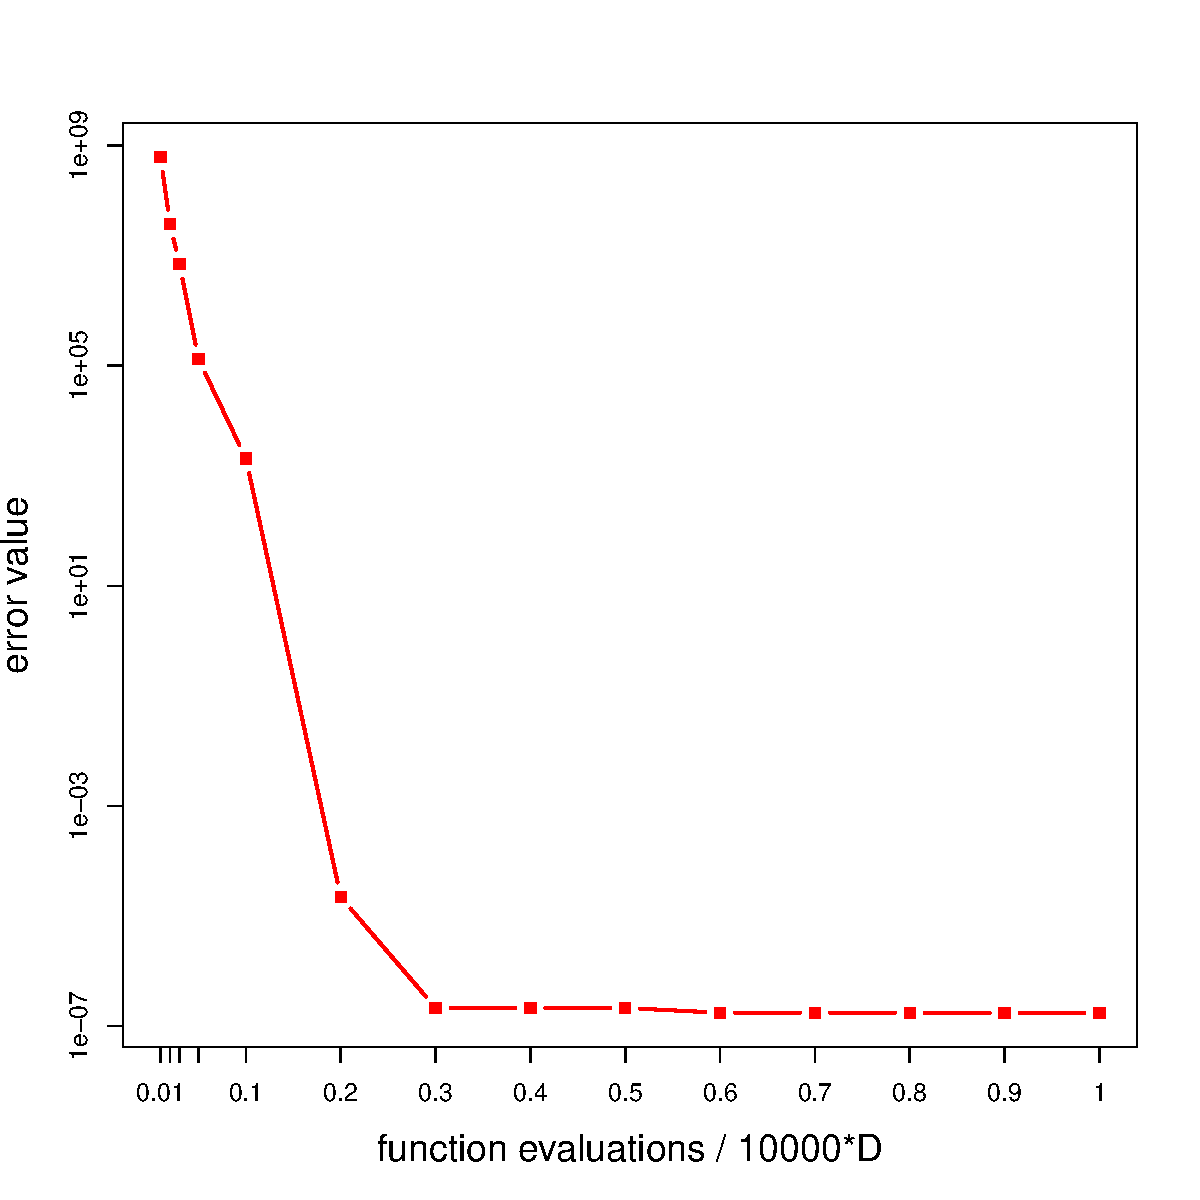
\includegraphics[width = \textwidth]{DESConvergence.pdf}
\caption{Convergence plot for a single run, with 14 budget steps on which error values have been reported. }
\label{fig:left}
\end{subfigure}
\begin{subfigure}{0.49\textwidth}
\vspace{-5mm}
\centering
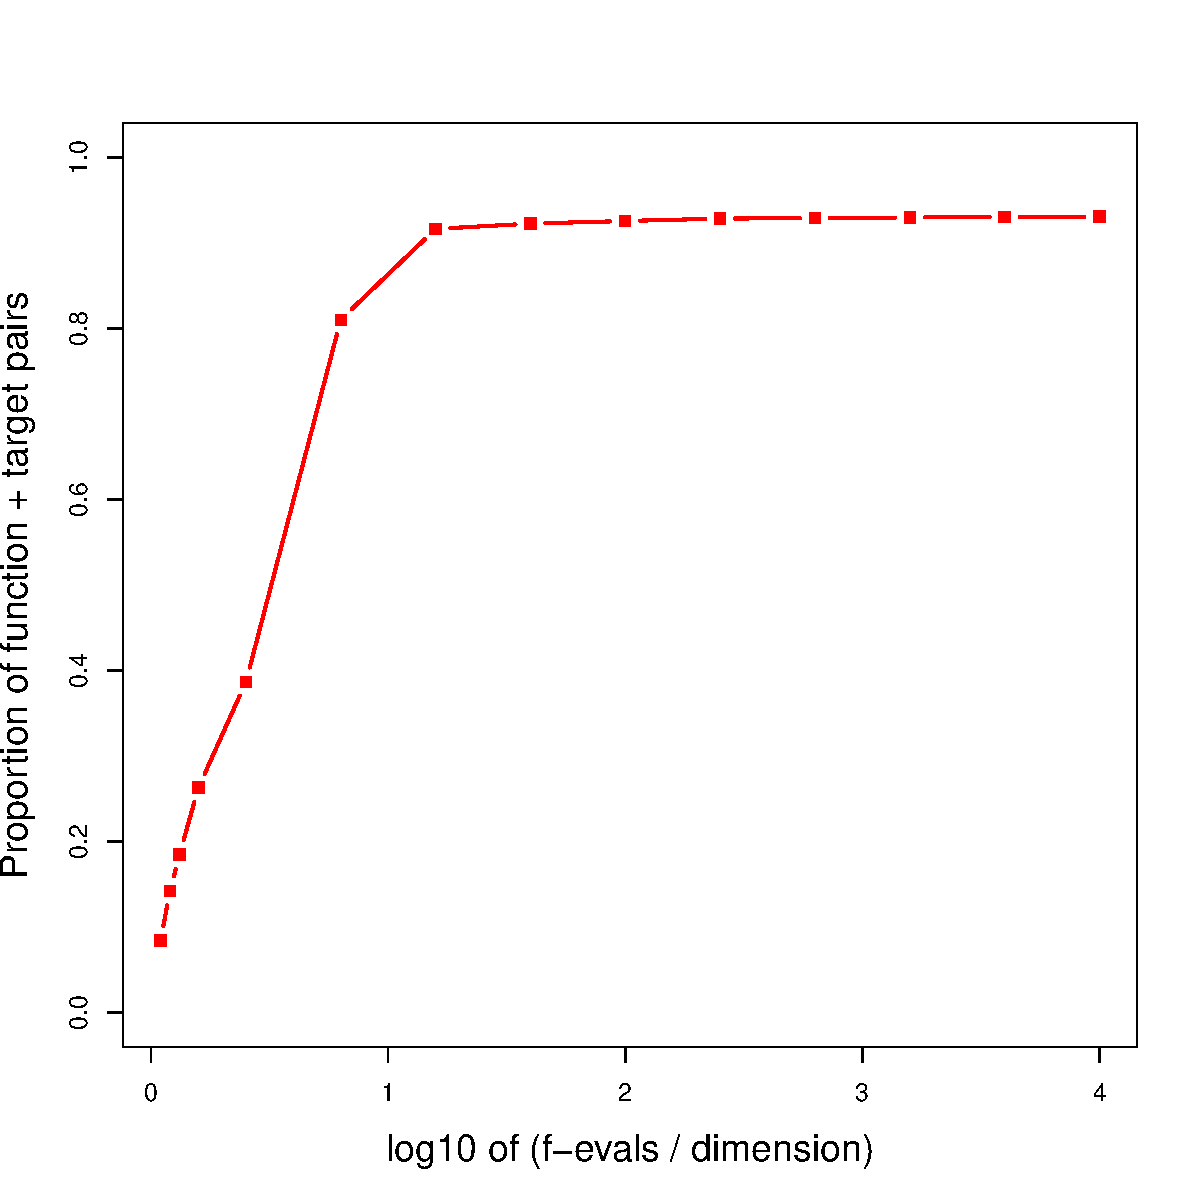
\includegraphics[width = \textwidth]{DESEcdf.pdf}
\caption{ECDF plot aggregated for 51 runs, for a single problem: P=1, N=10.}
\label{fig:right}
\end{subfigure}
\label{fig:combined}
\end{figure}
\vspace{-3mm}
We can see in right plot, for example, that about \textcolor{red}{90 percent} of the problems were solved within $10^2*D = 10^3$ function evaluations.

\end{frame}

\section{Results}
\begin{frame}
%\frametitle{CEC2017 Function 1}
\AddToShipoutPictureFG*{
    \AtPageUpperLeft{\put(-135,-12){
    \makebox[\paperwidth][r]{\textcolor{blue}{CEC2017 Function 1}}
    }
    }  
    }%

\begin{figure}[ht] 
    \vspace{-2mm}
\captionsetup[subfigure]{labelformat=empty}
  \begin{subfigure}[b]{0.5\linewidth}
    \centering
      \rotatebox[origin=c]{-90}{
        \begin{minipage}{1\linewidth}
    		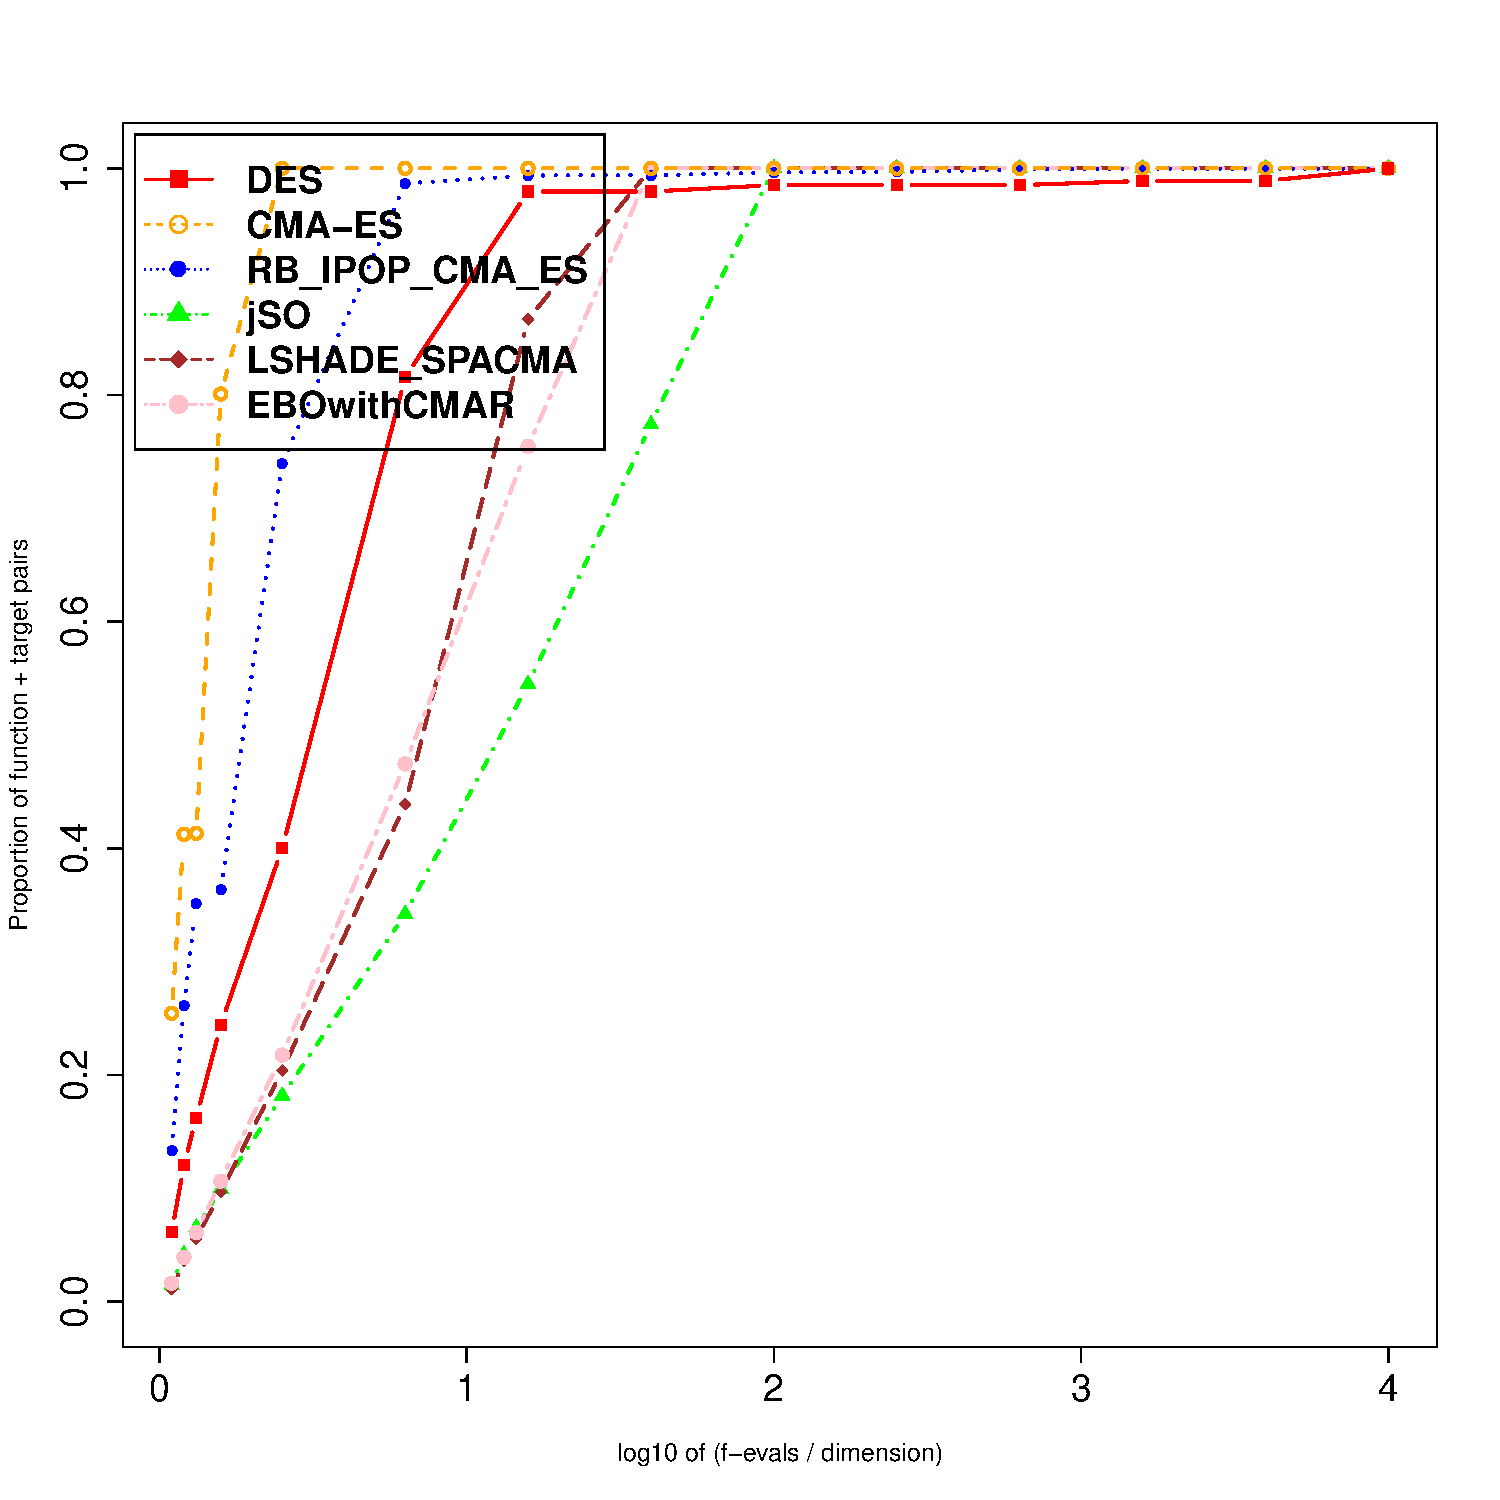
\includegraphics[height=0.9\linewidth,angle=90]{C:/Users/JS/Desktop/Doktorat/EvolutionAlgorithms/IEEEecdf/Plots/singlePlots/Problem=1,N=10.pdf} 
    		\caption{D=10} 
      	\end{minipage}%
	}
    \vspace{-12mm}
  \end{subfigure}%% 
  \begin{subfigure}[b]{0.5\linewidth}
    \centering
    \rotatebox[origin=c]{-90}{
        \begin{minipage}{1\linewidth}
            	\caption{D=30}
    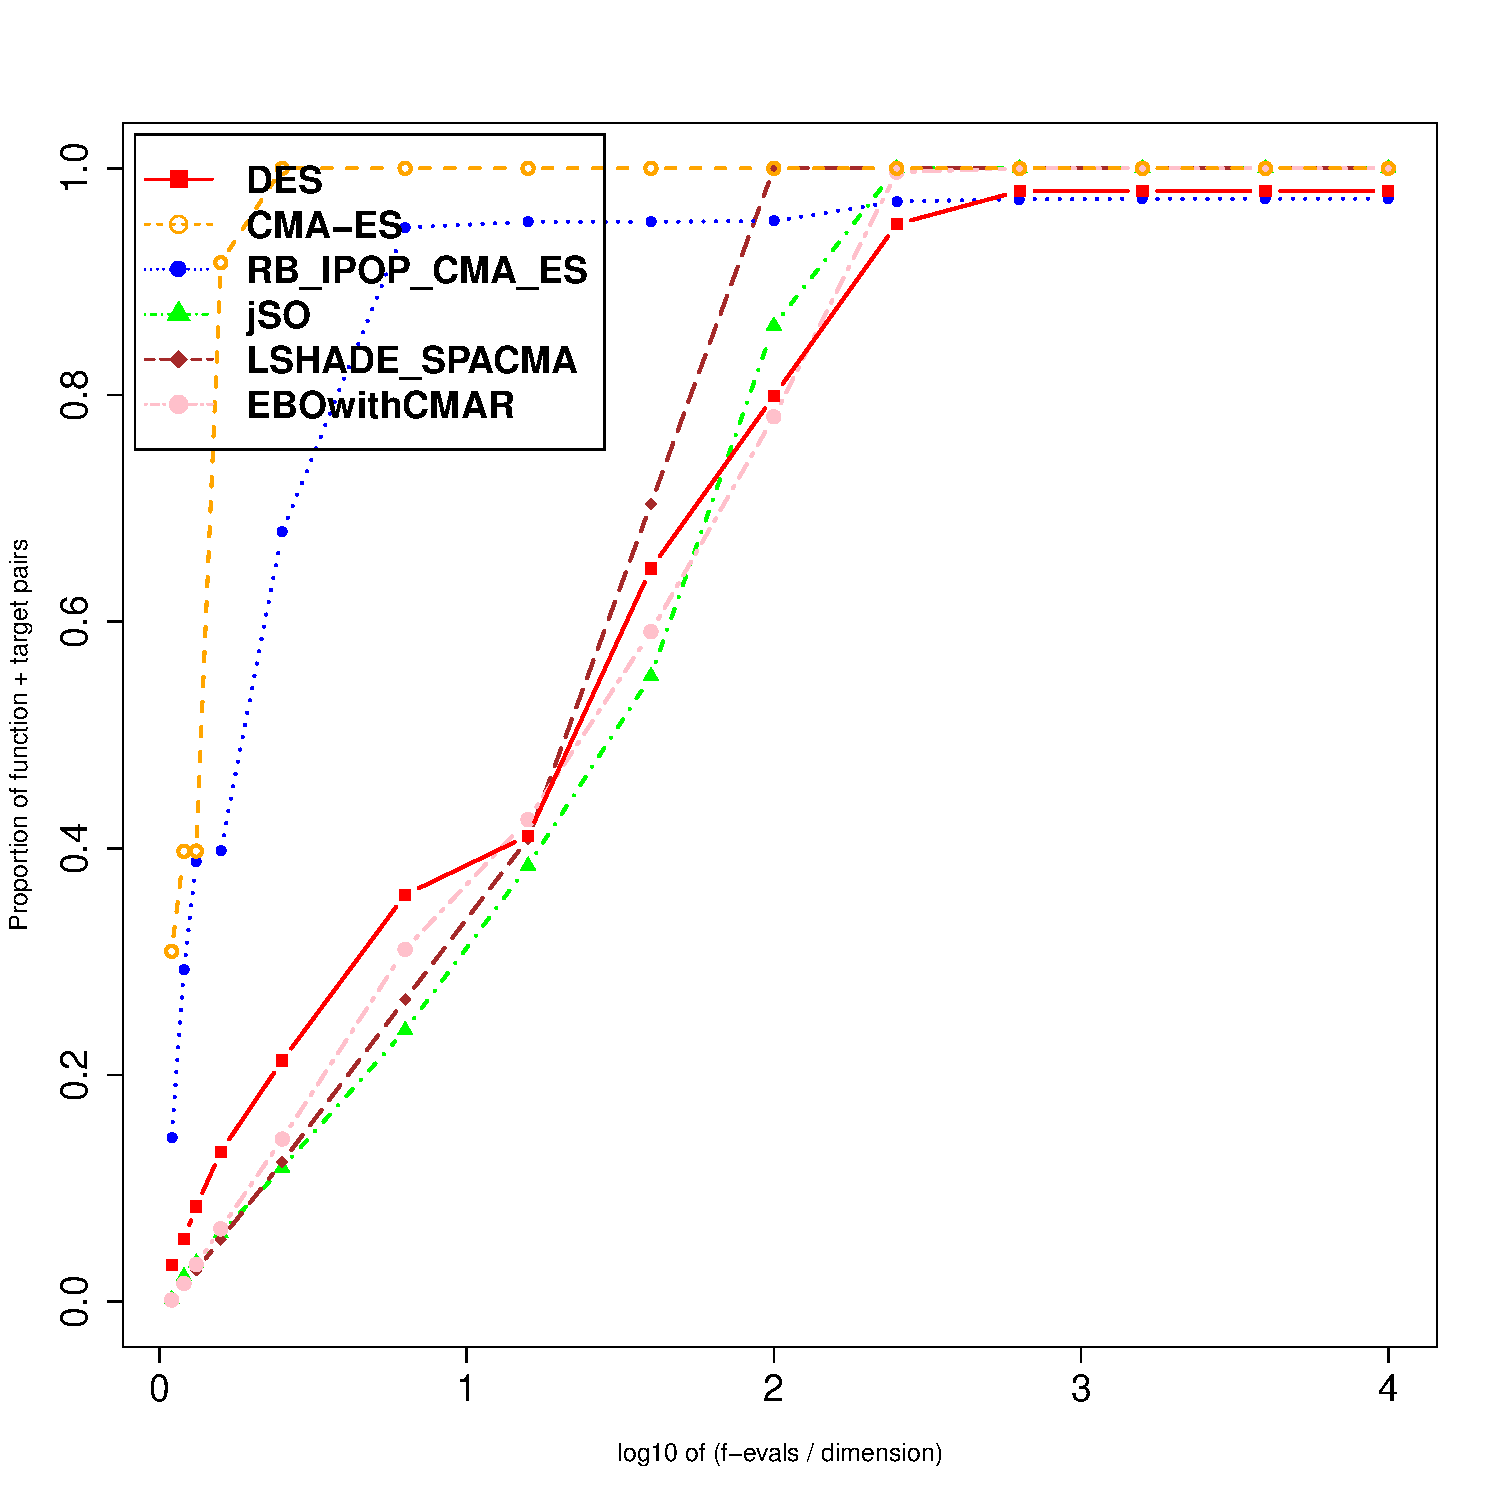
\includegraphics[height=0.9\linewidth,angle=90]{C:/Users/JS/Desktop/Doktorat/EvolutionAlgorithms/IEEEecdf/Plots/singlePlots/Problem=1,N=30.pdf} 
    	\end{minipage}%
	} 
    \vspace{-12mm}
  \end{subfigure} 
  \begin{subfigure}[b]{0.5\linewidth}
    \centering
    \rotatebox[origin=c]{-90}{
        \begin{minipage}{1\linewidth}
    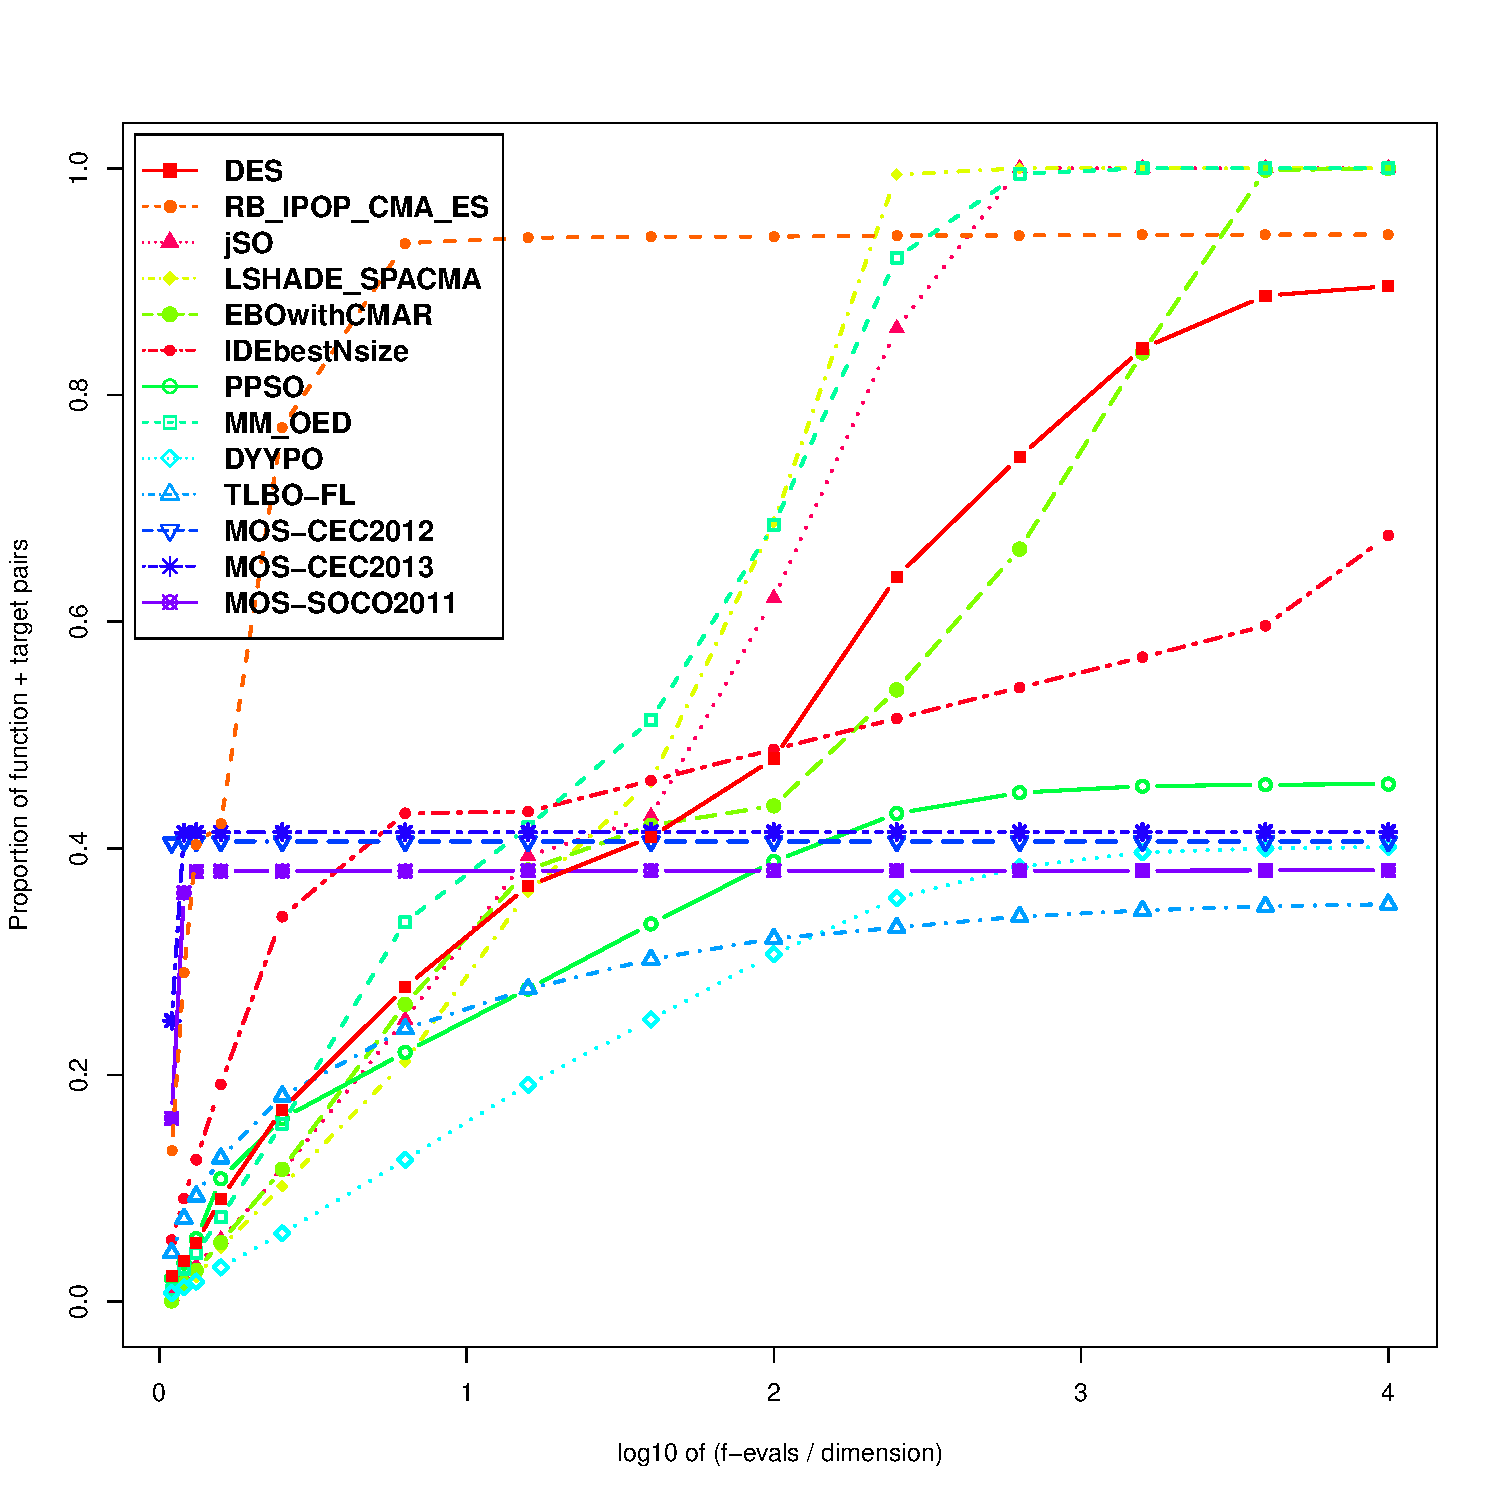
\includegraphics[height=0.9\linewidth,angle=90]{C:/Users/JS/Desktop/Doktorat/EvolutionAlgorithms/IEEEecdf/Plots/singlePlots/Problem=1,N=50.pdf} 
    	\caption{D=50}
    	\end{minipage}%
	}  
  \end{subfigure}%%
  \begin{subfigure}[b]{0.5\linewidth}
    \centering
    \rotatebox[origin=c]{-90}{
        \begin{minipage}{1\linewidth}
        \caption{D=100} 
    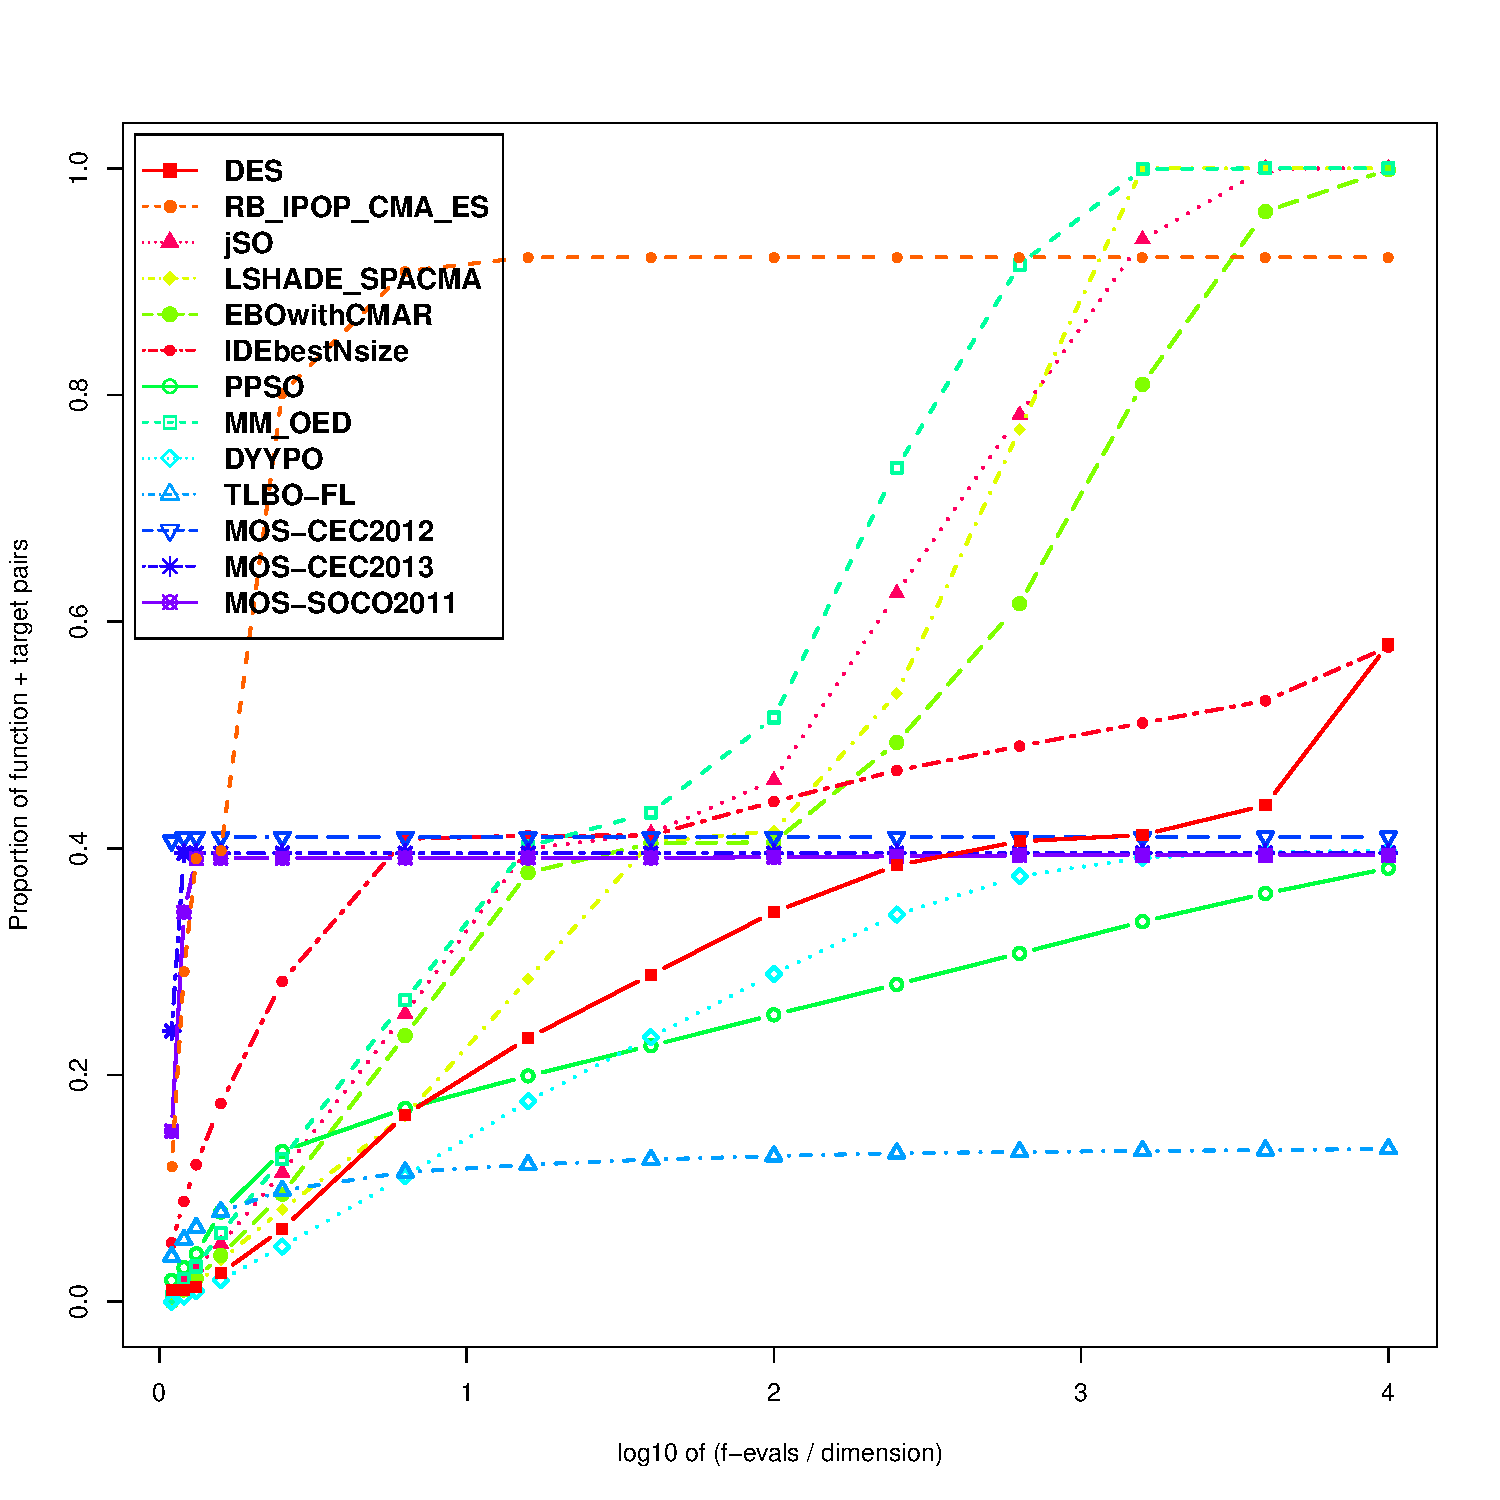
\includegraphics[height=0.9\linewidth,angle=90]{C:/Users/JS/Desktop/Doktorat/EvolutionAlgorithms/IEEEecdf/Plots/singlePlots/Problem=1,N=100.pdf}
    \end{minipage}%
	}   
  \end{subfigure} 
\end{figure}

\end{frame}

\begin{frame}
%\frametitle{CEC2017 Function 2}
\AddToShipoutPictureFG*{
    \AtPageUpperLeft{\put(-135,-12){
    \makebox[\paperwidth][r]{\textcolor{blue}{CEC2017 Function 2}}
    }
    }  
    }%

\begin{figure}[ht] 
    \vspace{-2mm}
\captionsetup[subfigure]{labelformat=empty}
  \begin{subfigure}[b]{0.5\linewidth}
    \centering
      \rotatebox[origin=c]{-90}{
        \begin{minipage}{1\linewidth}
    		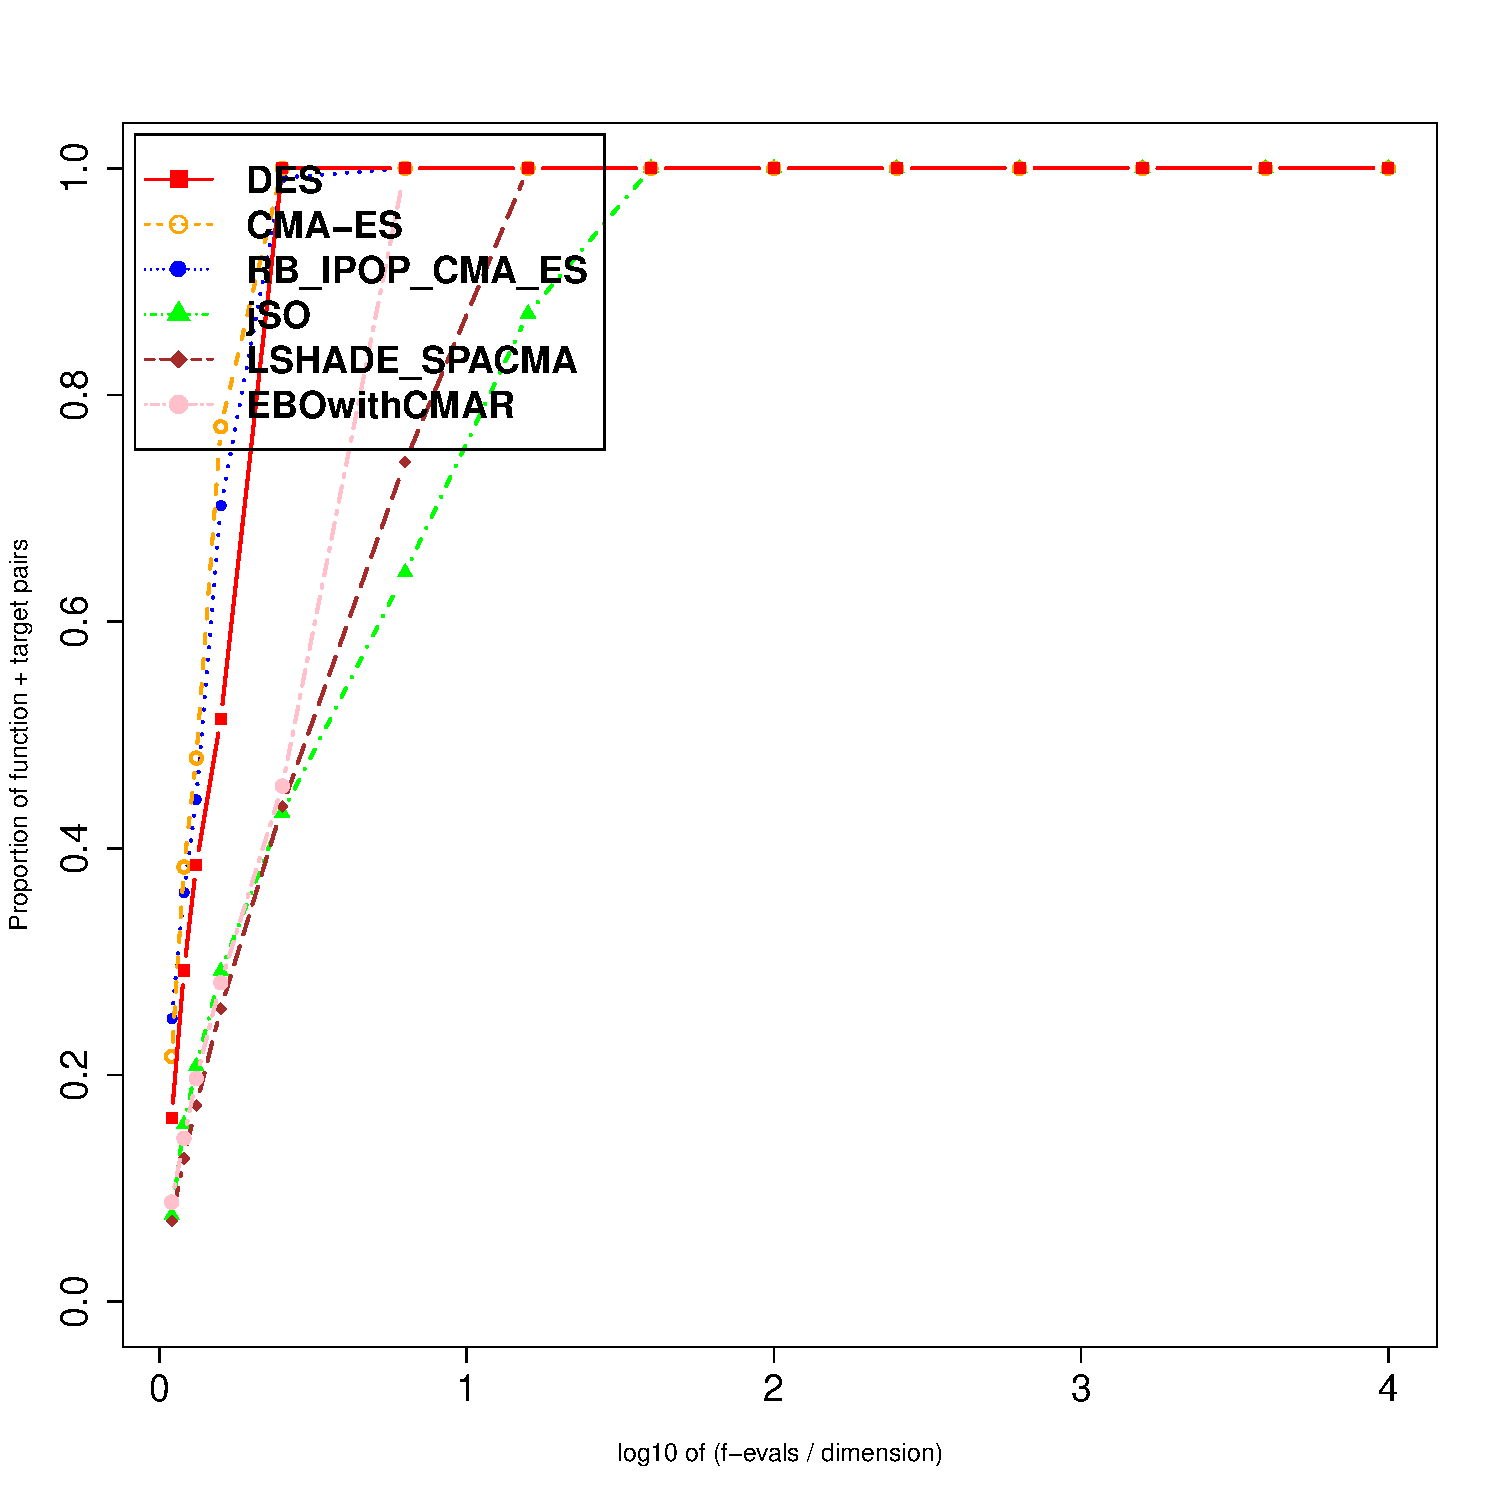
\includegraphics[height=0.9\linewidth,angle=90]{C:/Users/JS/Desktop/Doktorat/EvolutionAlgorithms/IEEEecdf/Plots/singlePlots/Problem=2,N=10.pdf} 
    		\caption{D=10} 
      	\end{minipage}%
	}
    \vspace{-12mm}
  \end{subfigure}%% 
  \begin{subfigure}[b]{0.5\linewidth}
    \centering
    \rotatebox[origin=c]{-90}{
        \begin{minipage}{1\linewidth}
            	\caption{D=30}
    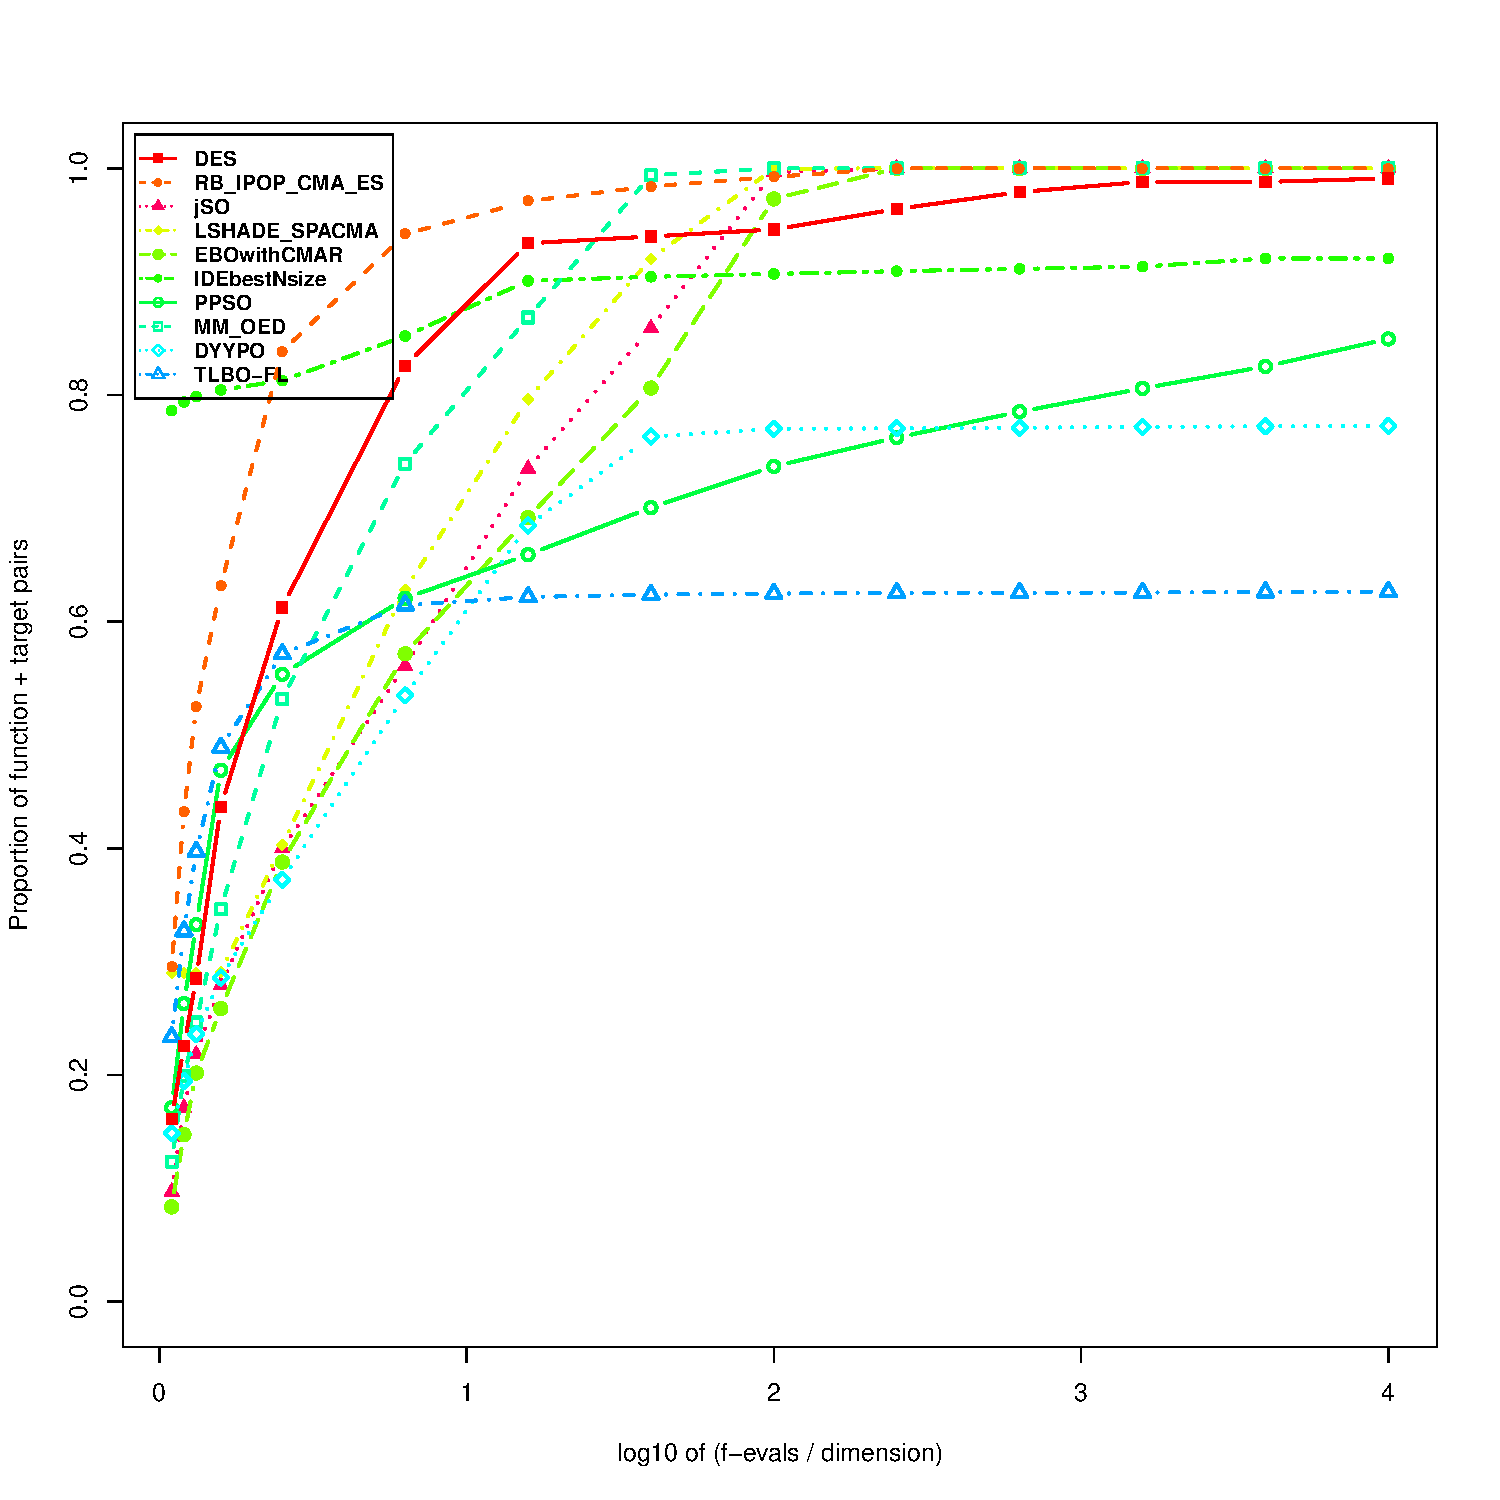
\includegraphics[height=0.9\linewidth,angle=90]{C:/Users/JS/Desktop/Doktorat/EvolutionAlgorithms/IEEEecdf/Plots/singlePlots/Problem=2,N=30.pdf} 
    	\end{minipage}%
	} 
    \vspace{-12mm}
  \end{subfigure} 
  \begin{subfigure}[b]{0.5\linewidth}
    \centering
    \rotatebox[origin=c]{-90}{
        \begin{minipage}{1\linewidth}
    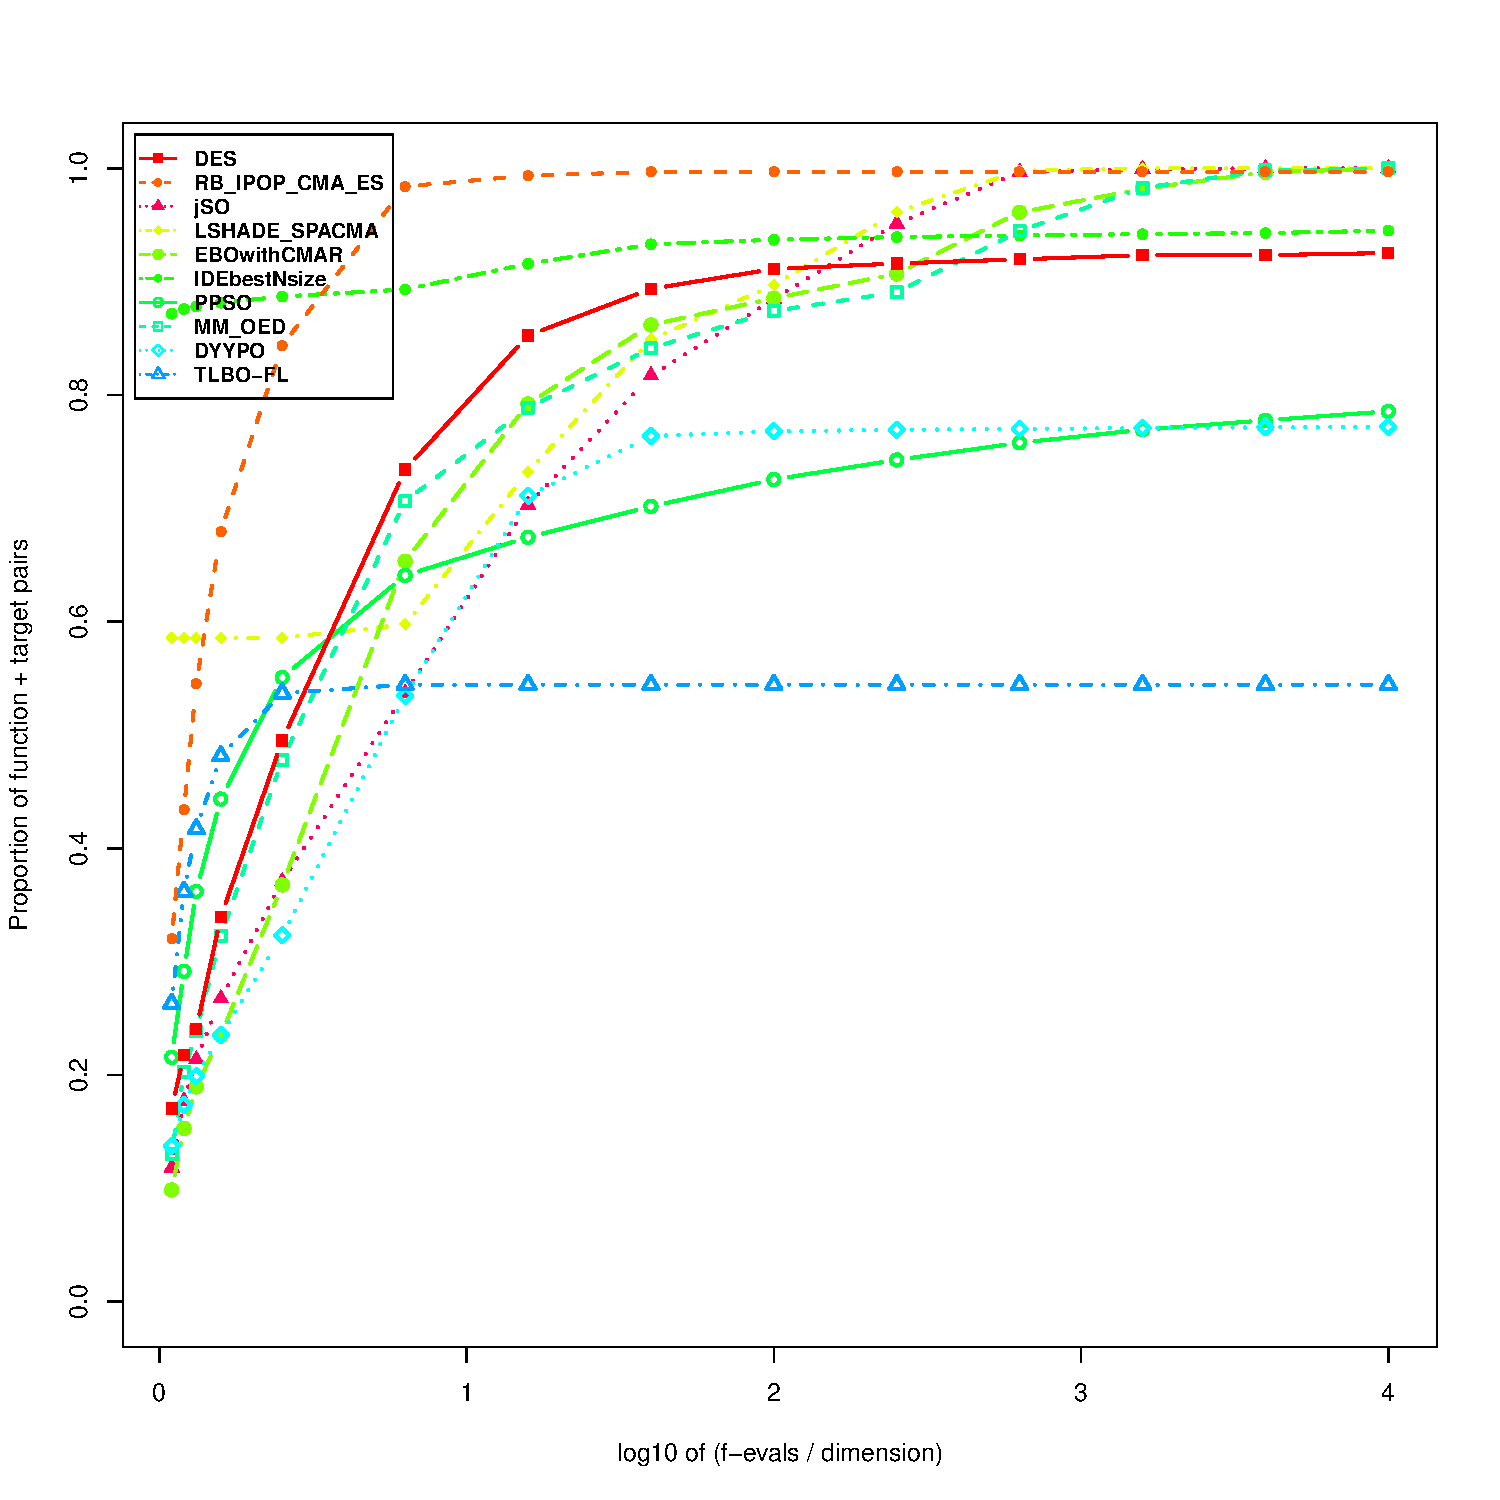
\includegraphics[height=0.9\linewidth,angle=90]{C:/Users/JS/Desktop/Doktorat/EvolutionAlgorithms/IEEEecdf/Plots/singlePlots/Problem=2,N=50.pdf} 
    	\caption{D=50}
    	\end{minipage}%
	}  
  \end{subfigure}%%
  \begin{subfigure}[b]{0.5\linewidth}
    \centering
    \rotatebox[origin=c]{-90}{
        \begin{minipage}{1\linewidth}
        \caption{D=100} 
    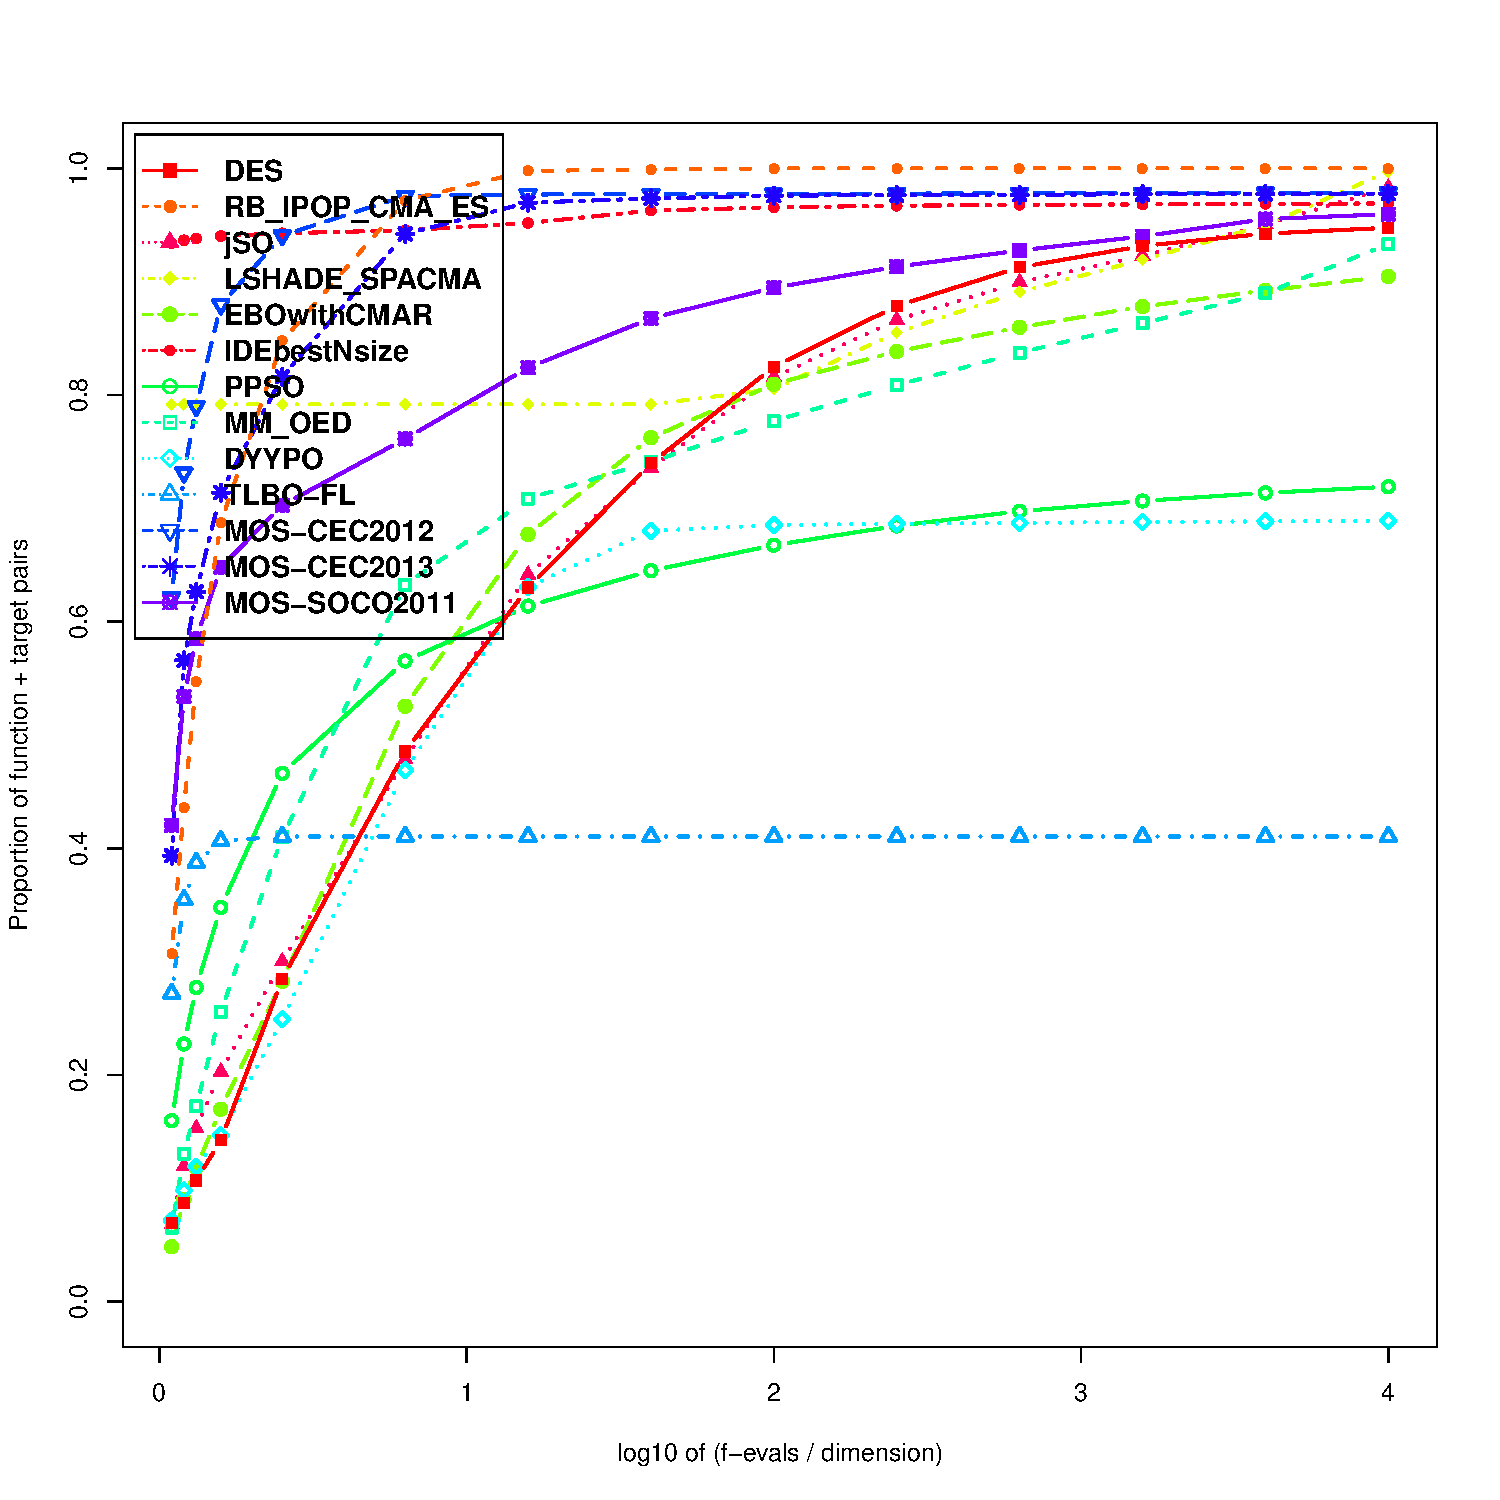
\includegraphics[height=0.9\linewidth,angle=90]{C:/Users/JS/Desktop/Doktorat/EvolutionAlgorithms/IEEEecdf/Plots/singlePlots/Problem=2,N=100.pdf}
    \end{minipage}%
	}   
  \end{subfigure} 
\end{figure}

\end{frame}


\begin{frame}
%\frametitle{CEC2017 Function 3}
\AddToShipoutPictureFG*{
    \AtPageUpperLeft{\put(-135,-12){
    \makebox[\paperwidth][r]{\textcolor{blue}{CEC2017 Function 3}}
    }
    }  
    }%

\begin{figure}[ht] 
    \vspace{-2mm}
\captionsetup[subfigure]{labelformat=empty}
  \begin{subfigure}[b]{0.5\linewidth}
    \centering
      \rotatebox[origin=c]{-90}{
        \begin{minipage}{1\linewidth}
    		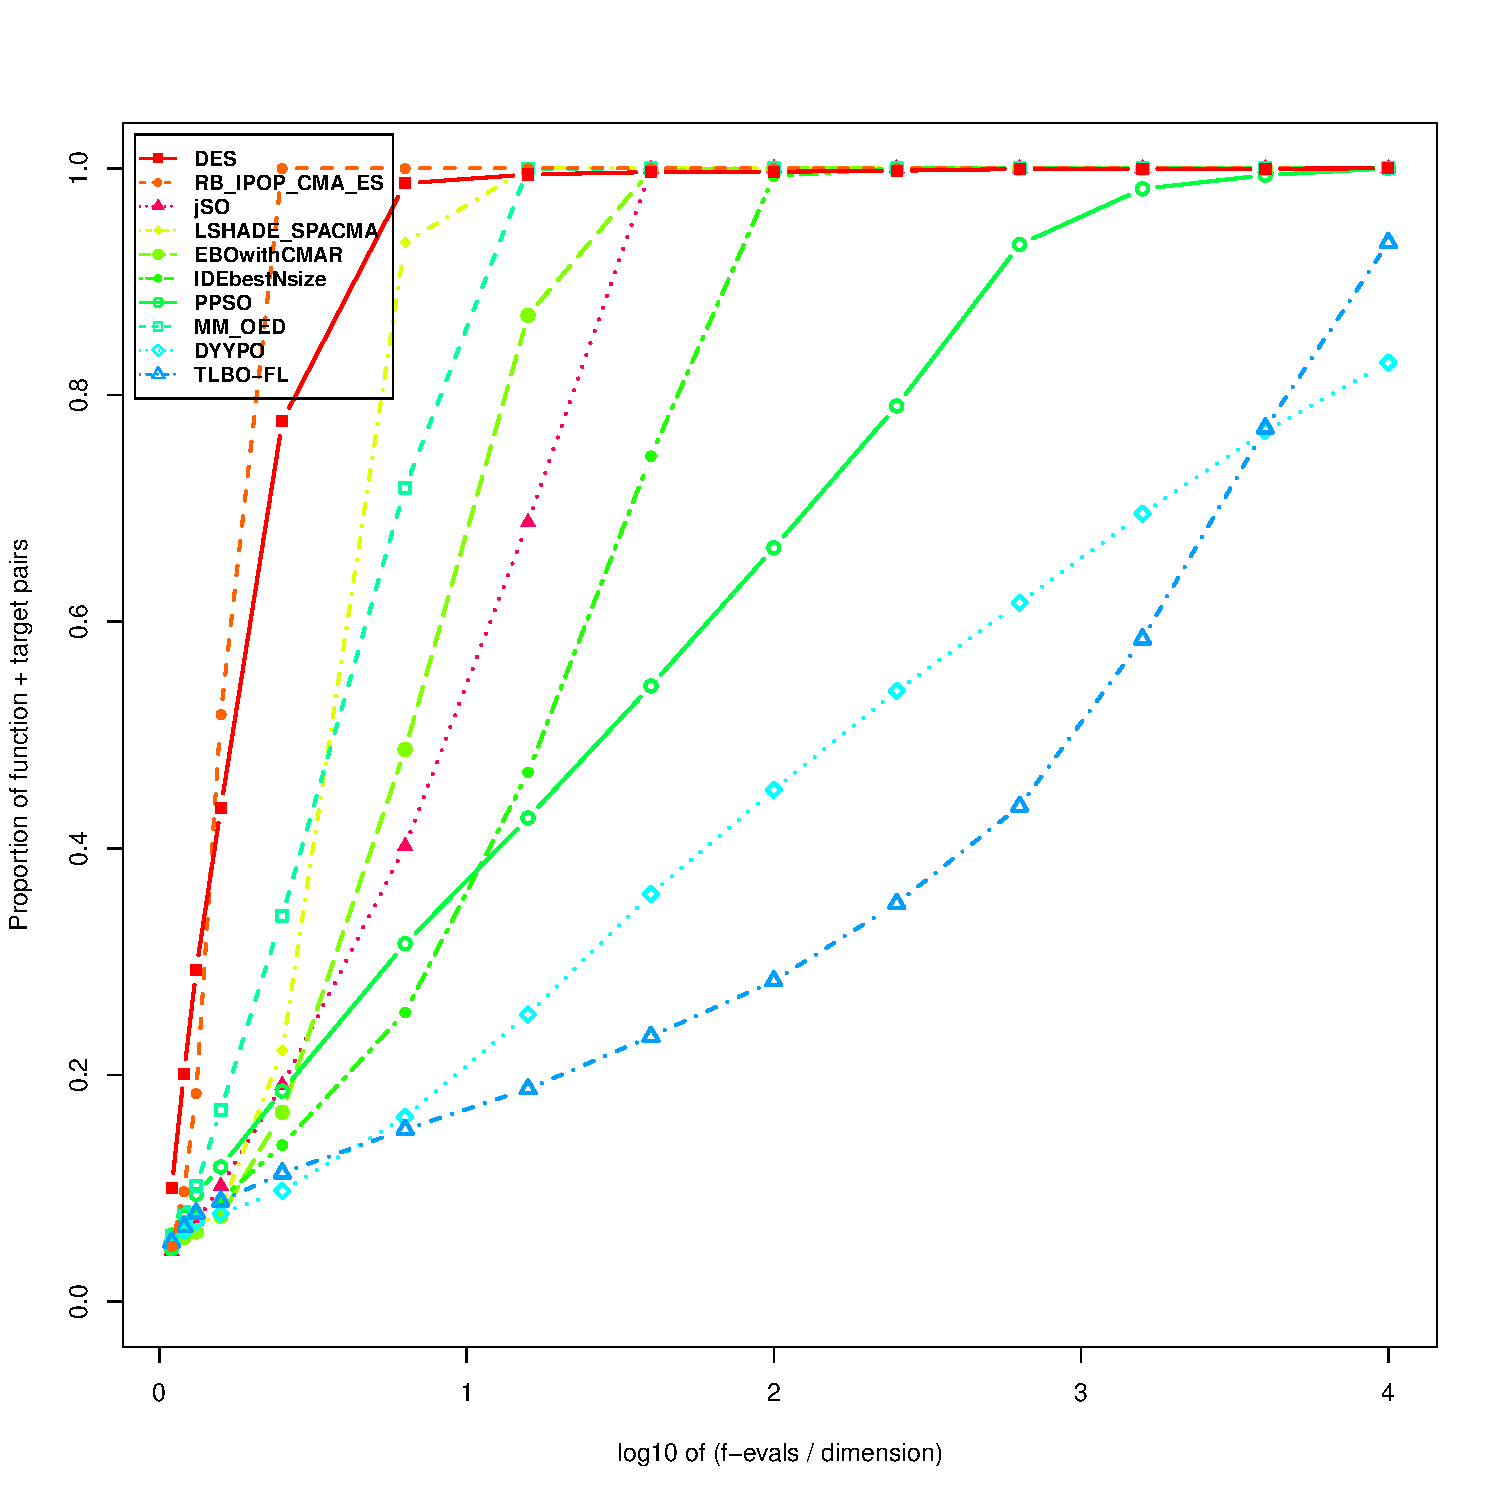
\includegraphics[height=0.9\linewidth,angle=90]{C:/Users/JS/Desktop/Doktorat/EvolutionAlgorithms/IEEEecdf/Plots/singlePlots/Problem=3,N=10.pdf} 
    		\caption{D=10} 
      	\end{minipage}%
	}
    \vspace{-12mm}
  \end{subfigure}%% 
  \begin{subfigure}[b]{0.5\linewidth}
    \centering
    \rotatebox[origin=c]{-90}{
        \begin{minipage}{1\linewidth}
            	\caption{D=30}
    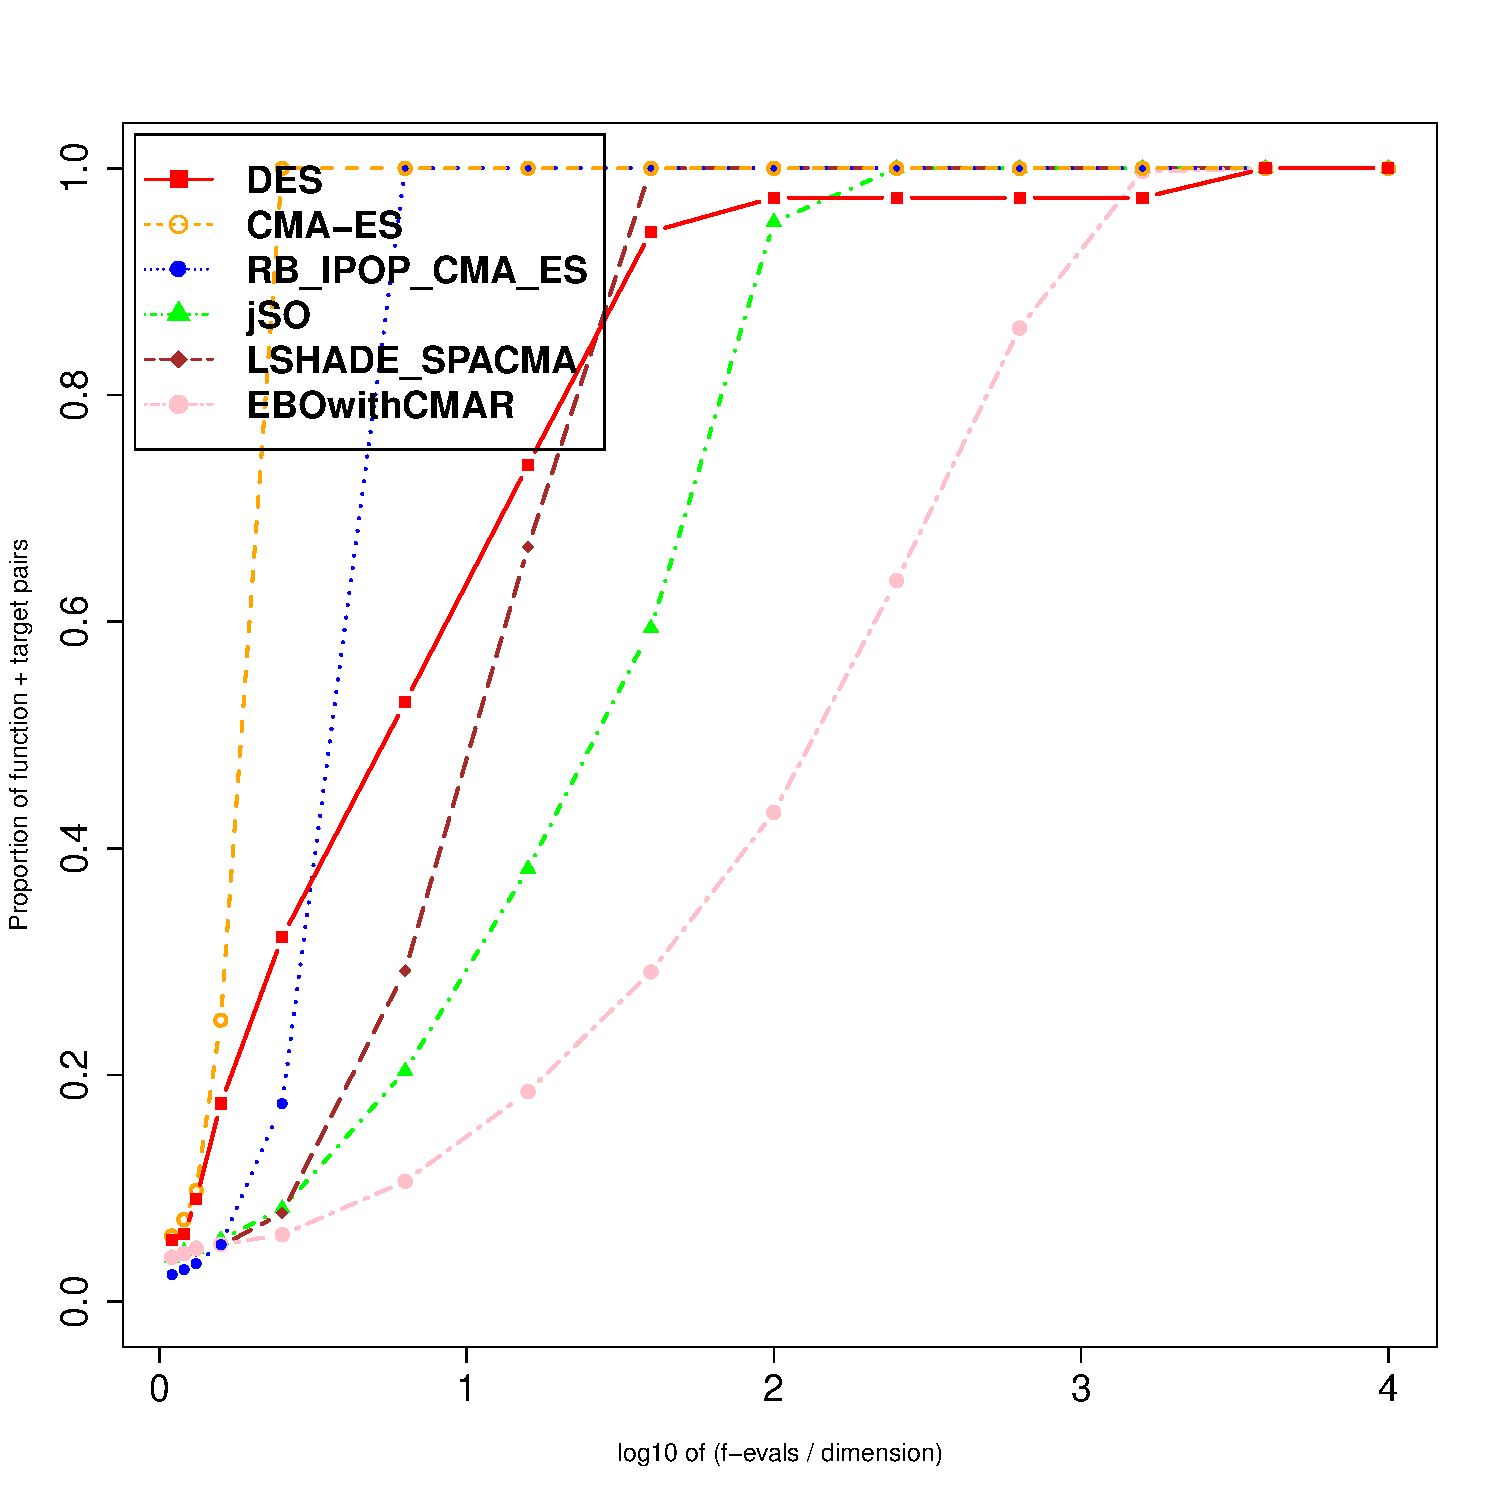
\includegraphics[height=0.9\linewidth,angle=90]{C:/Users/JS/Desktop/Doktorat/EvolutionAlgorithms/IEEEecdf/Plots/singlePlots/Problem=3,N=30.pdf} 
    	\end{minipage}%
	} 
    \vspace{-12mm}
  \end{subfigure} 
  \begin{subfigure}[b]{0.5\linewidth}
    \centering
    \rotatebox[origin=c]{-90}{
        \begin{minipage}{1\linewidth}
    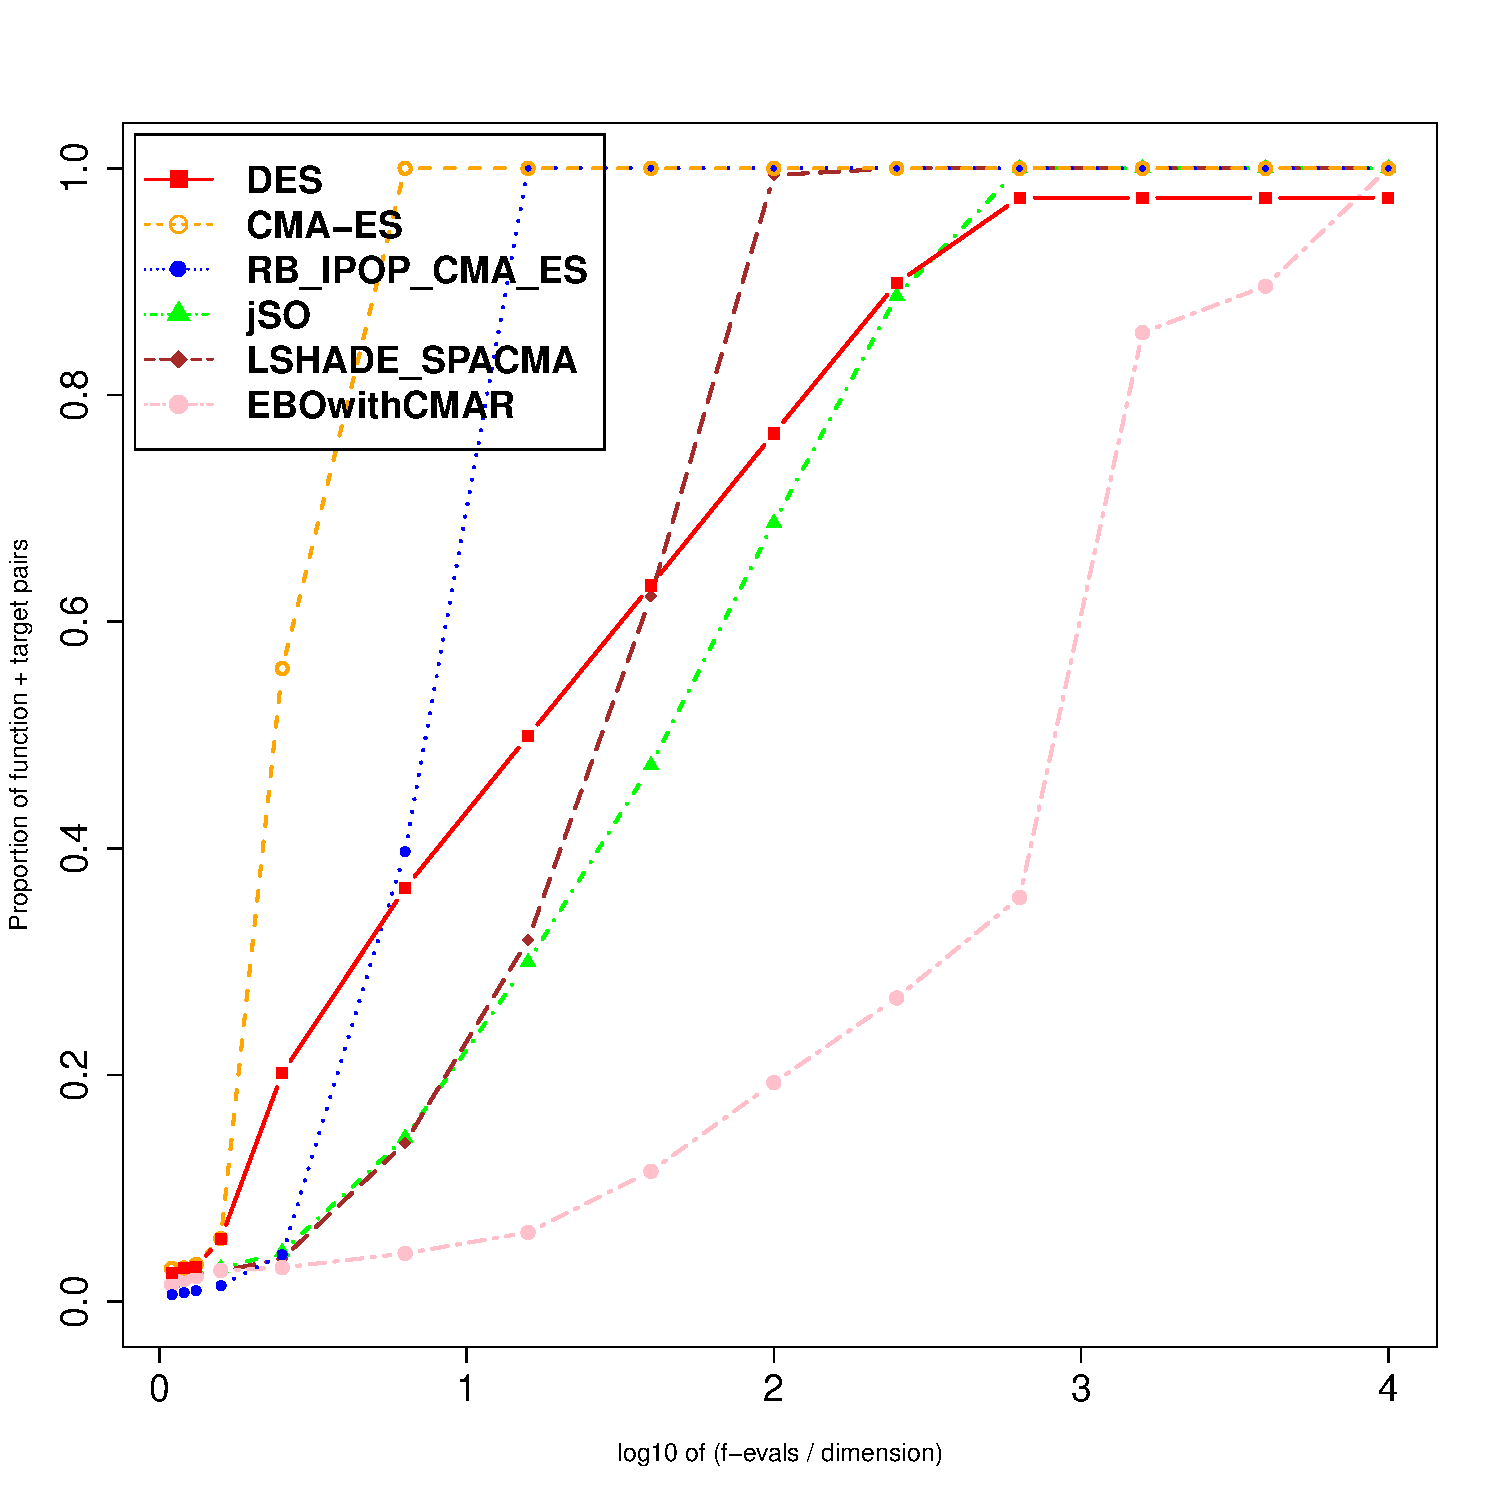
\includegraphics[height=0.9\linewidth,angle=90]{C:/Users/JS/Desktop/Doktorat/EvolutionAlgorithms/IEEEecdf/Plots/singlePlots/Problem=3,N=50.pdf} 
    	\caption{D=50}
    	\end{minipage}%
	}  
  \end{subfigure}%%
  \begin{subfigure}[b]{0.5\linewidth}
    \centering
    \rotatebox[origin=c]{-90}{
        \begin{minipage}{1\linewidth}
        \caption{D=100} 
    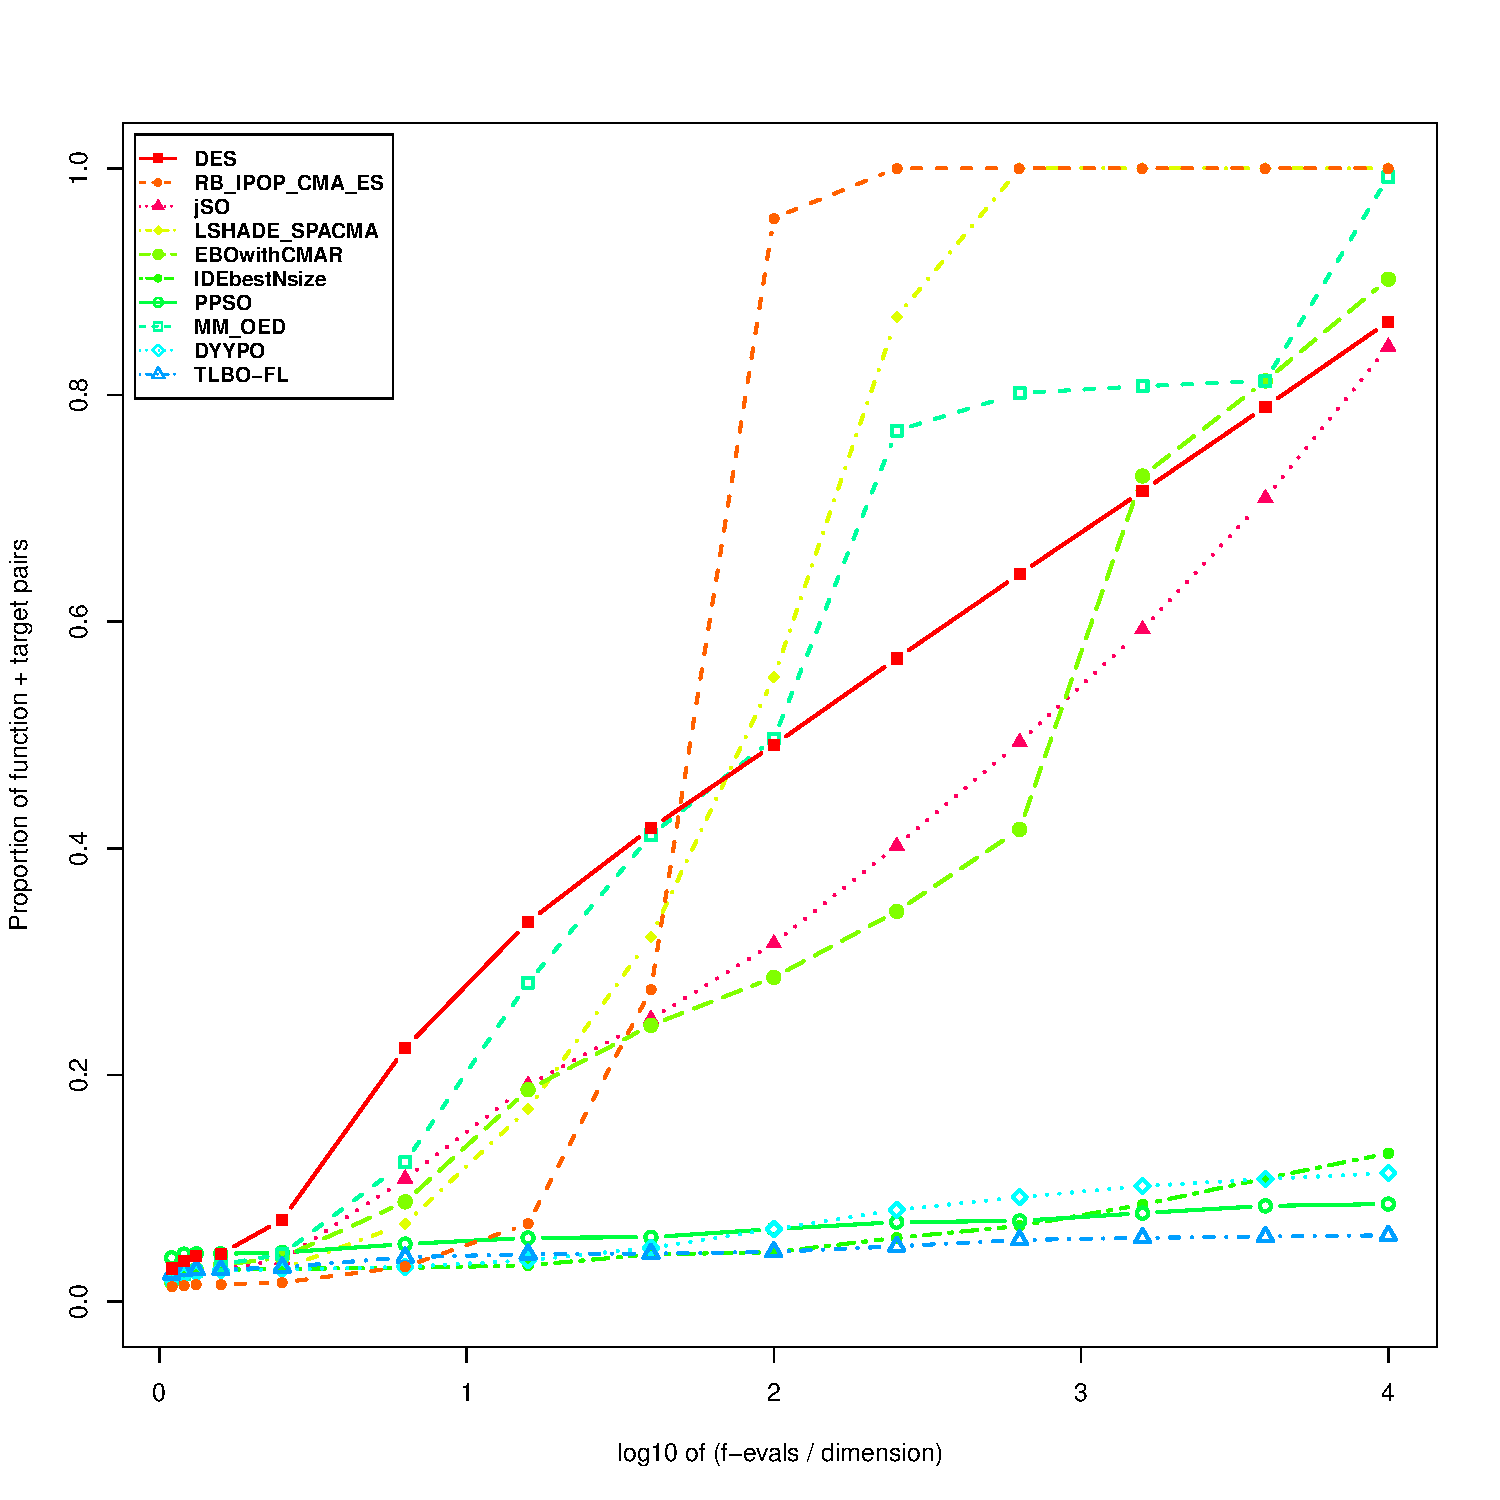
\includegraphics[height=0.9\linewidth,angle=90]{C:/Users/JS/Desktop/Doktorat/EvolutionAlgorithms/IEEEecdf/Plots/singlePlots/Problem=3,N=100.pdf}
    \end{minipage}%
	}   
  \end{subfigure} 
\end{figure}

\end{frame}


\begin{frame}
%\frametitle{CEC2017 Function 4}
\AddToShipoutPictureFG*{
    \AtPageUpperLeft{\put(-135,-12){
    \makebox[\paperwidth][r]{\textcolor{blue}{CEC2017 Function 4}}
    }
    }  
    }%

\begin{figure}[ht] 
    \vspace{-2mm}
\captionsetup[subfigure]{labelformat=empty}
  \begin{subfigure}[b]{0.5\linewidth}
    \centering
      \rotatebox[origin=c]{-90}{
        \begin{minipage}{1\linewidth}
    		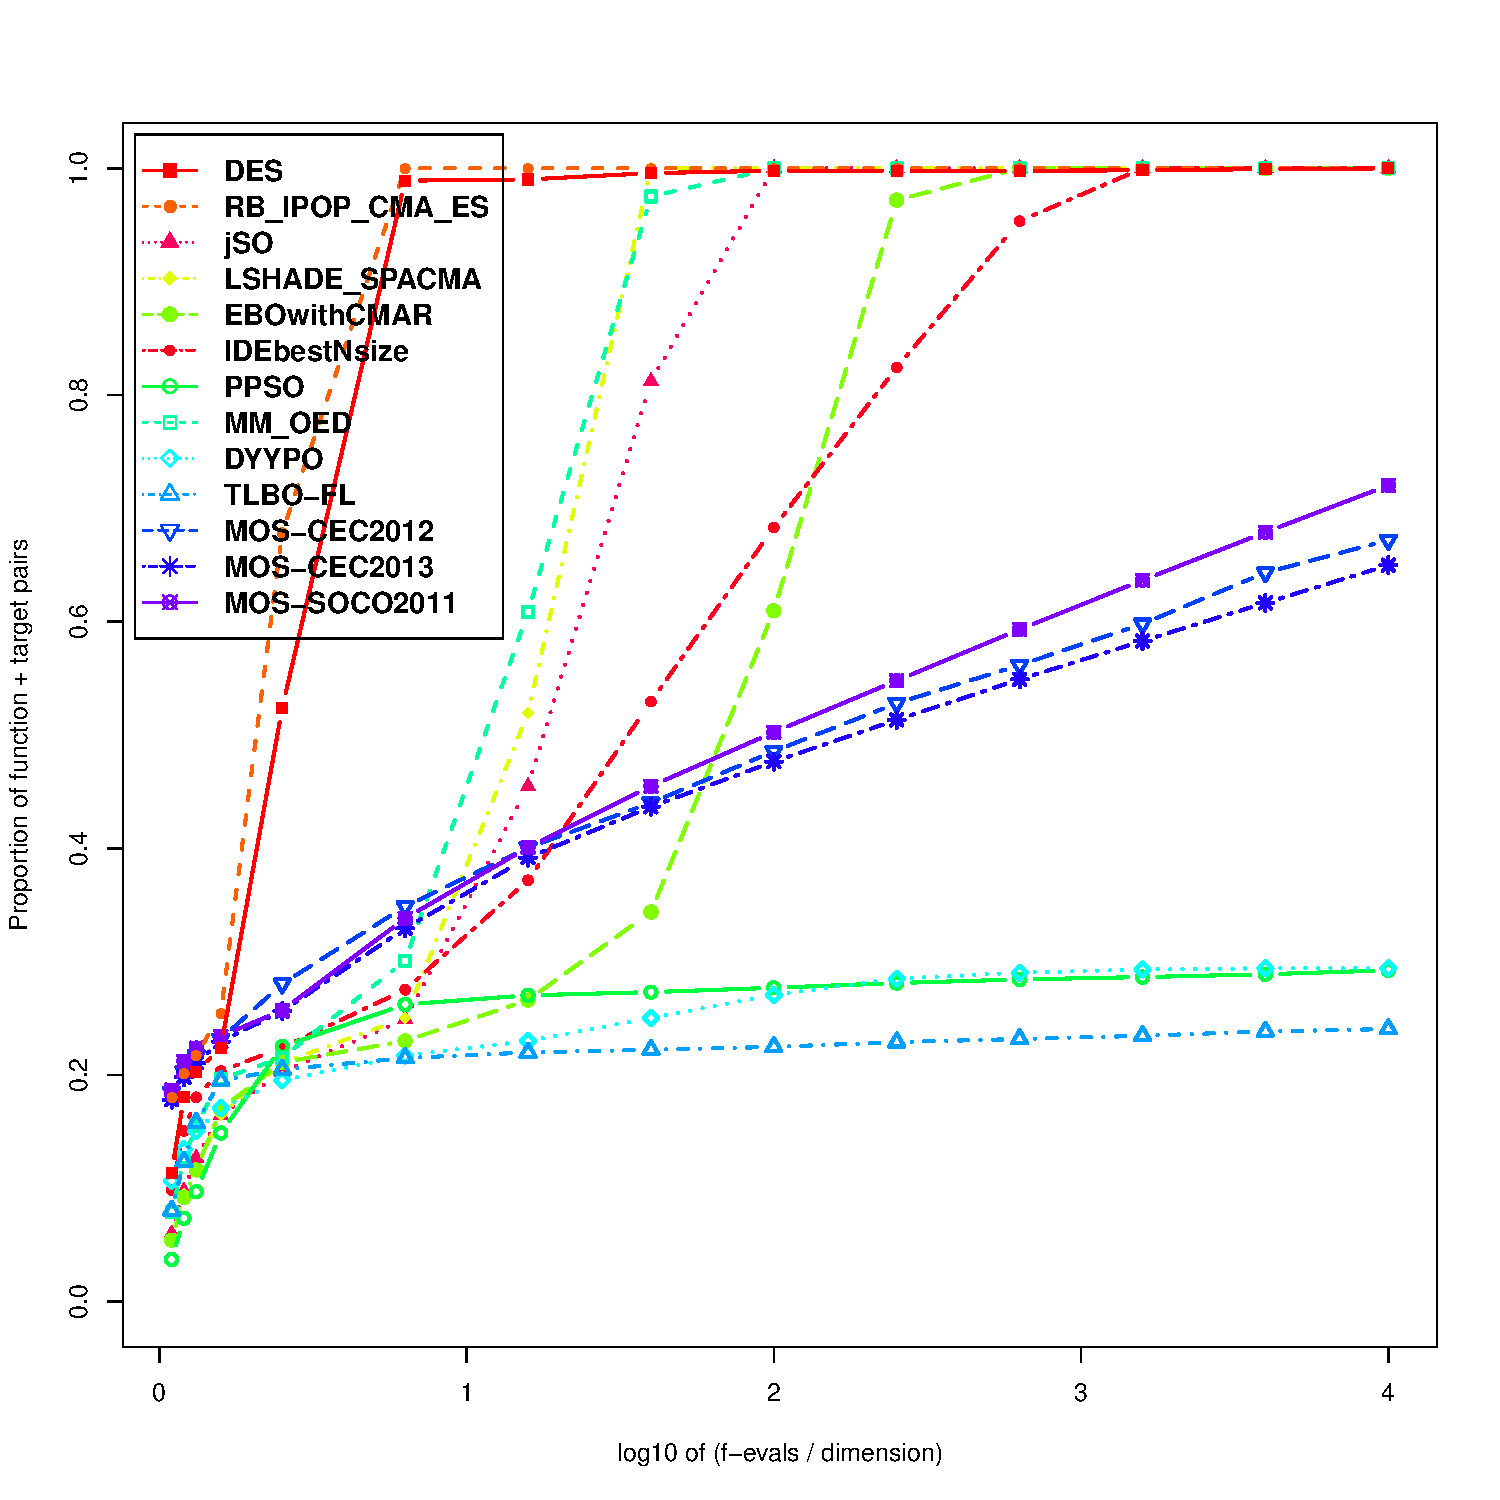
\includegraphics[height=0.9\linewidth,angle=90]{C:/Users/JS/Desktop/Doktorat/EvolutionAlgorithms/IEEEecdf/Plots/singlePlots/Problem=4,N=10.pdf} 
    		\caption{D=10} 
      	\end{minipage}%
	}
    \vspace{-12mm}
  \end{subfigure}%% 
  \begin{subfigure}[b]{0.5\linewidth}
    \centering
    \rotatebox[origin=c]{-90}{
        \begin{minipage}{1\linewidth}
            	\caption{D=30}
    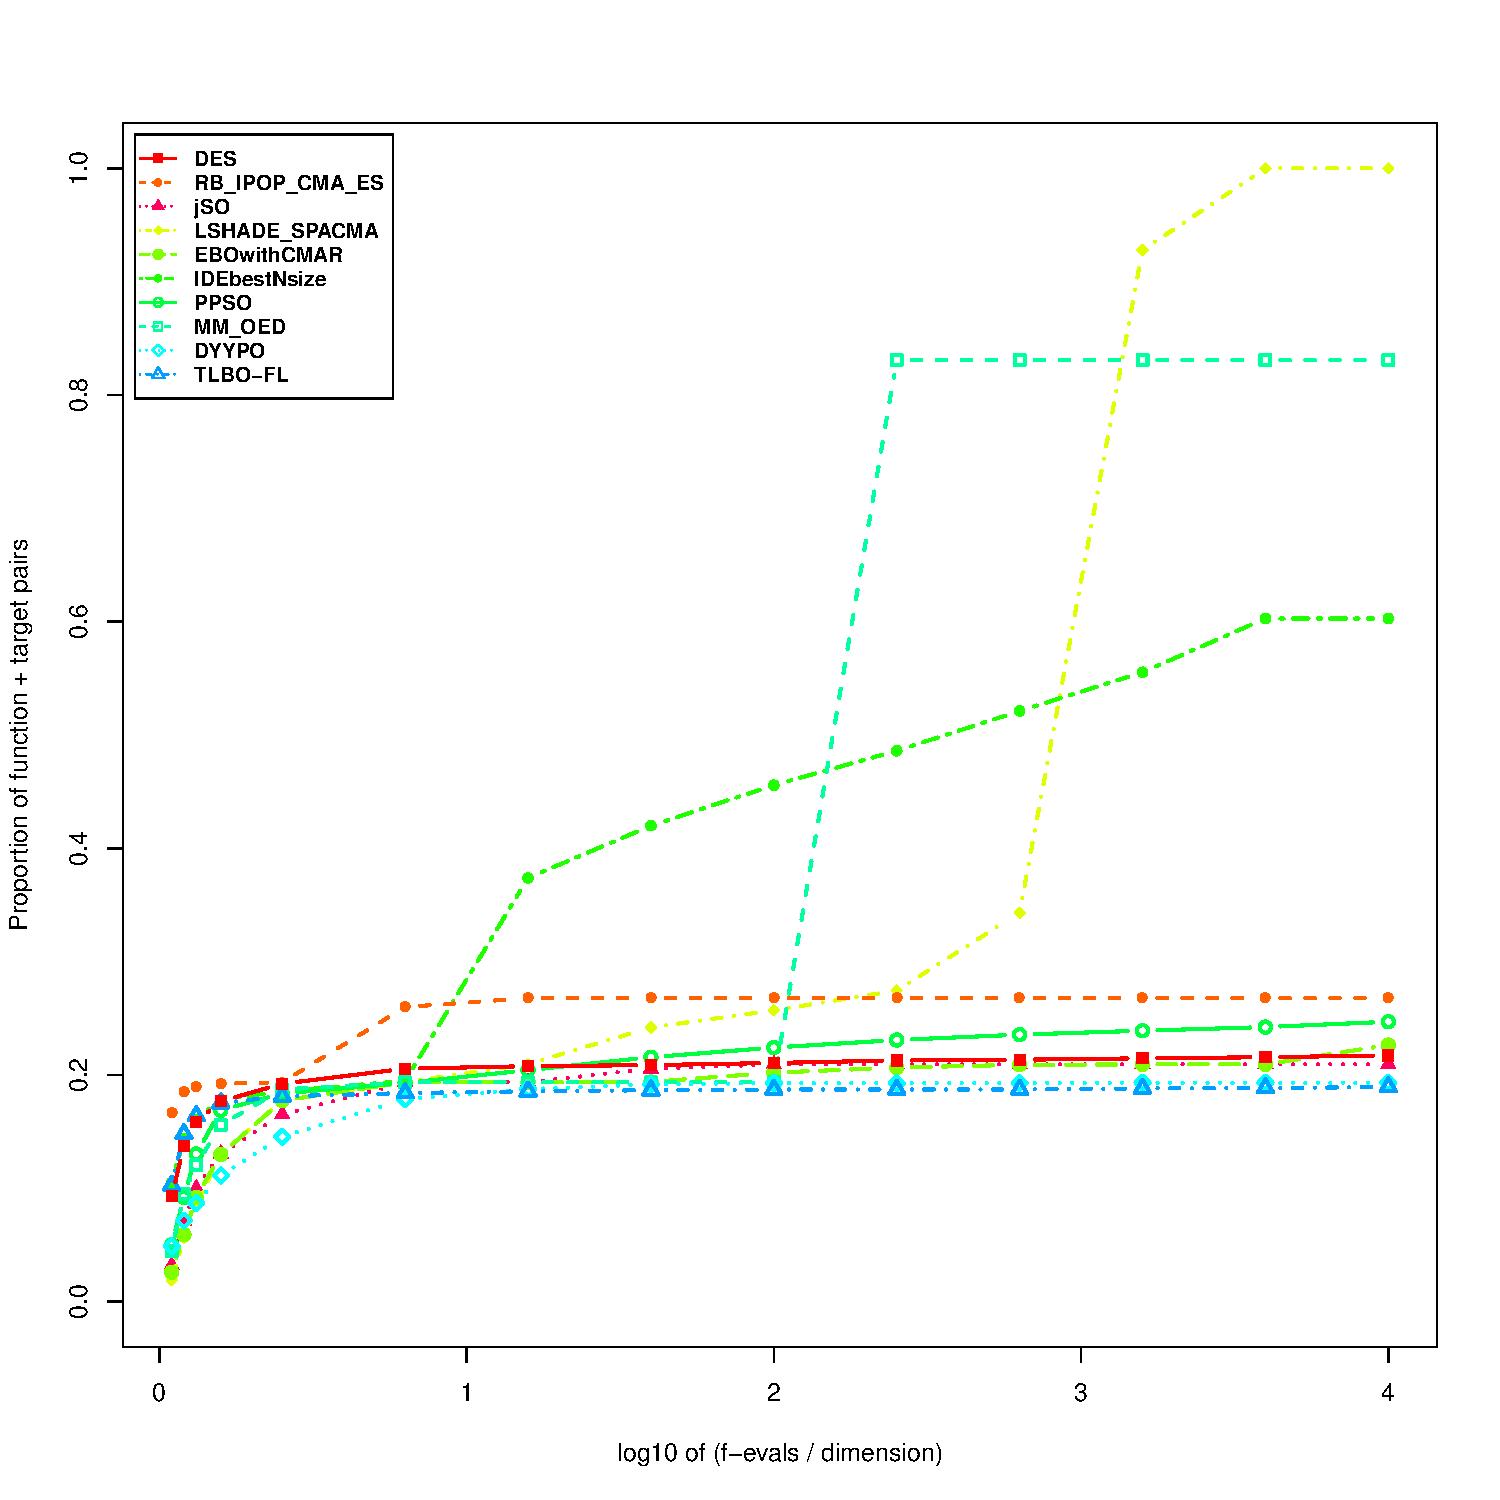
\includegraphics[height=0.9\linewidth,angle=90]{C:/Users/JS/Desktop/Doktorat/EvolutionAlgorithms/IEEEecdf/Plots/singlePlots/Problem=4,N=30.pdf} 
    	\end{minipage}%
	} 
    \vspace{-12mm}
  \end{subfigure} 
  \begin{subfigure}[b]{0.5\linewidth}
    \centering
    \rotatebox[origin=c]{-90}{
        \begin{minipage}{1\linewidth}
    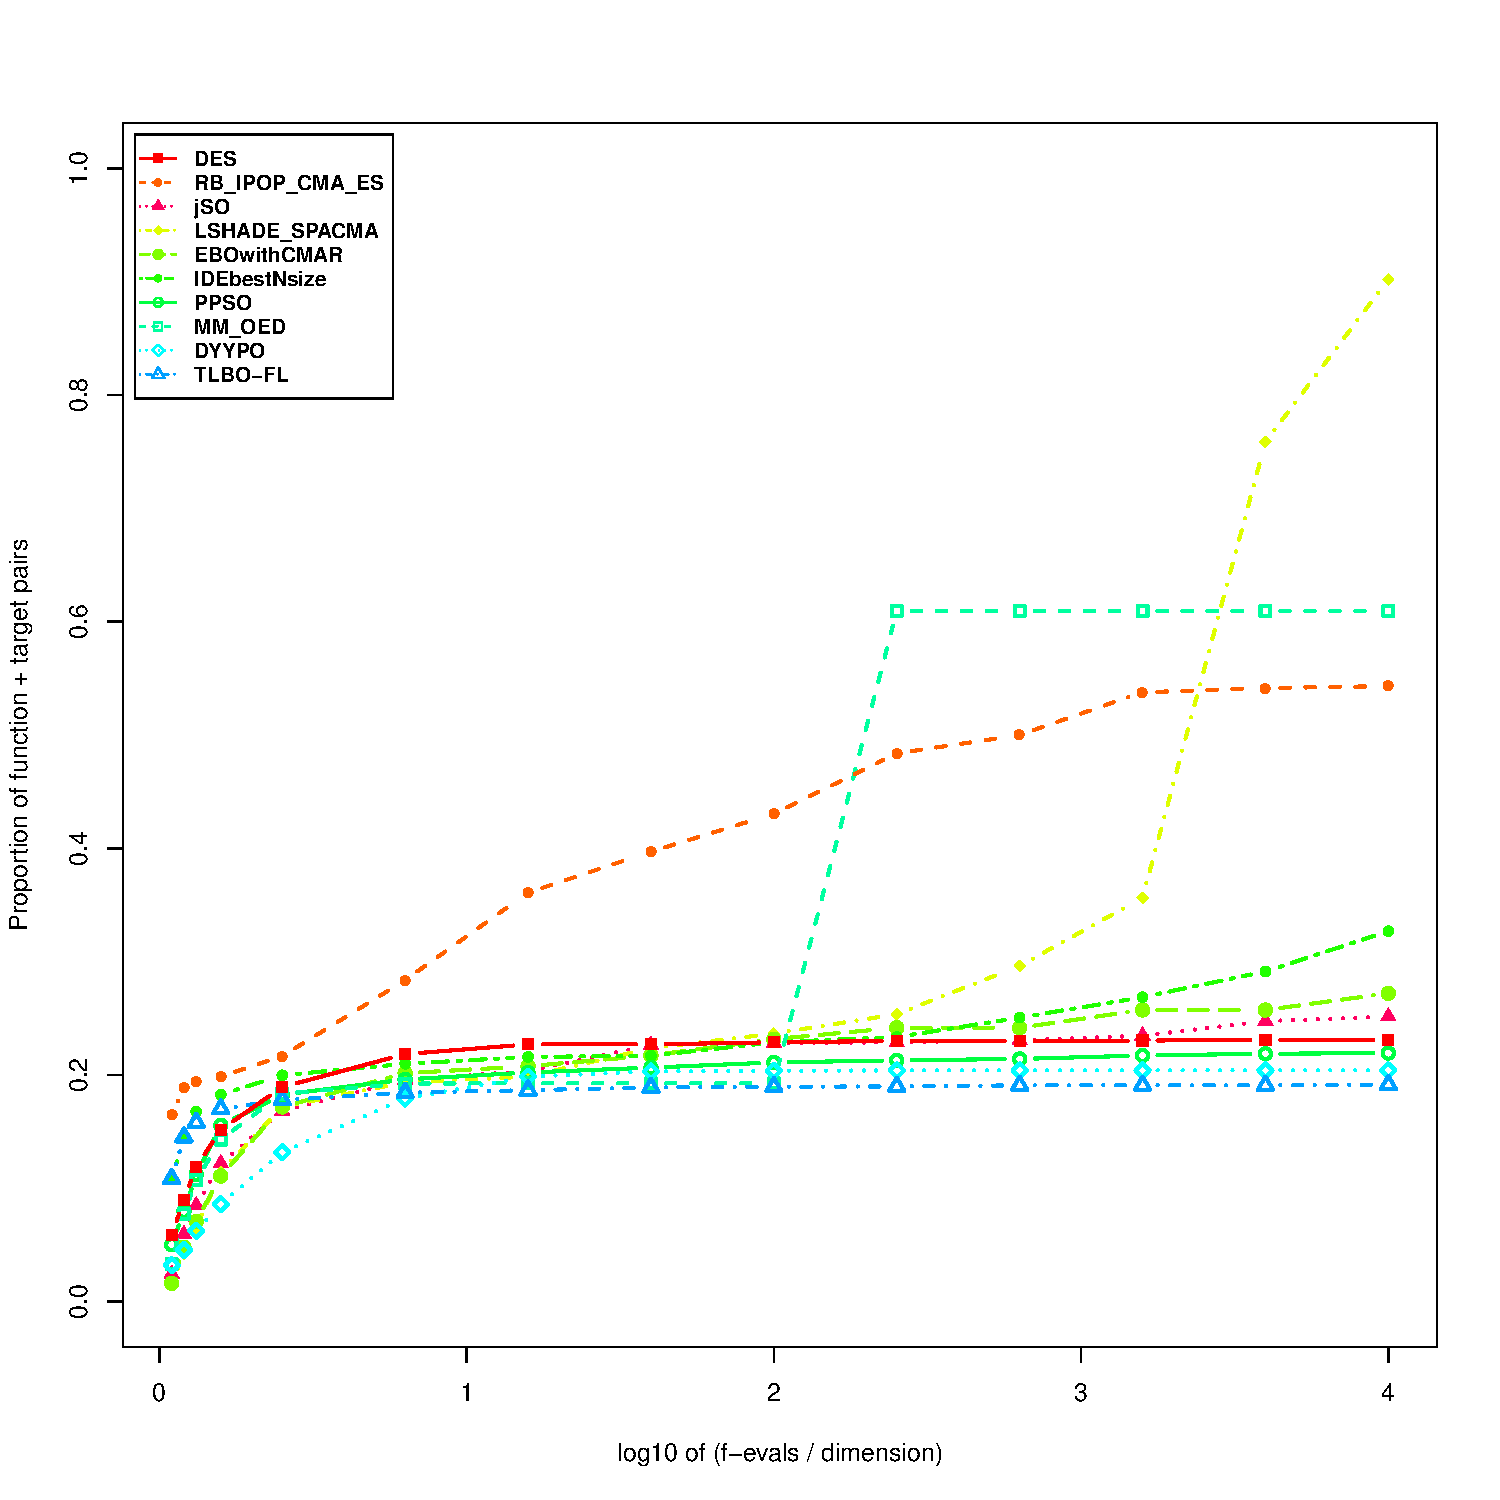
\includegraphics[height=0.9\linewidth,angle=90]{C:/Users/JS/Desktop/Doktorat/EvolutionAlgorithms/IEEEecdf/Plots/singlePlots/Problem=4,N=50.pdf} 
    	\caption{D=50}
    	\end{minipage}%
	}  
  \end{subfigure}%%
  \begin{subfigure}[b]{0.5\linewidth}
    \centering
    \rotatebox[origin=c]{-90}{
        \begin{minipage}{1\linewidth}
        \caption{D=100} 
    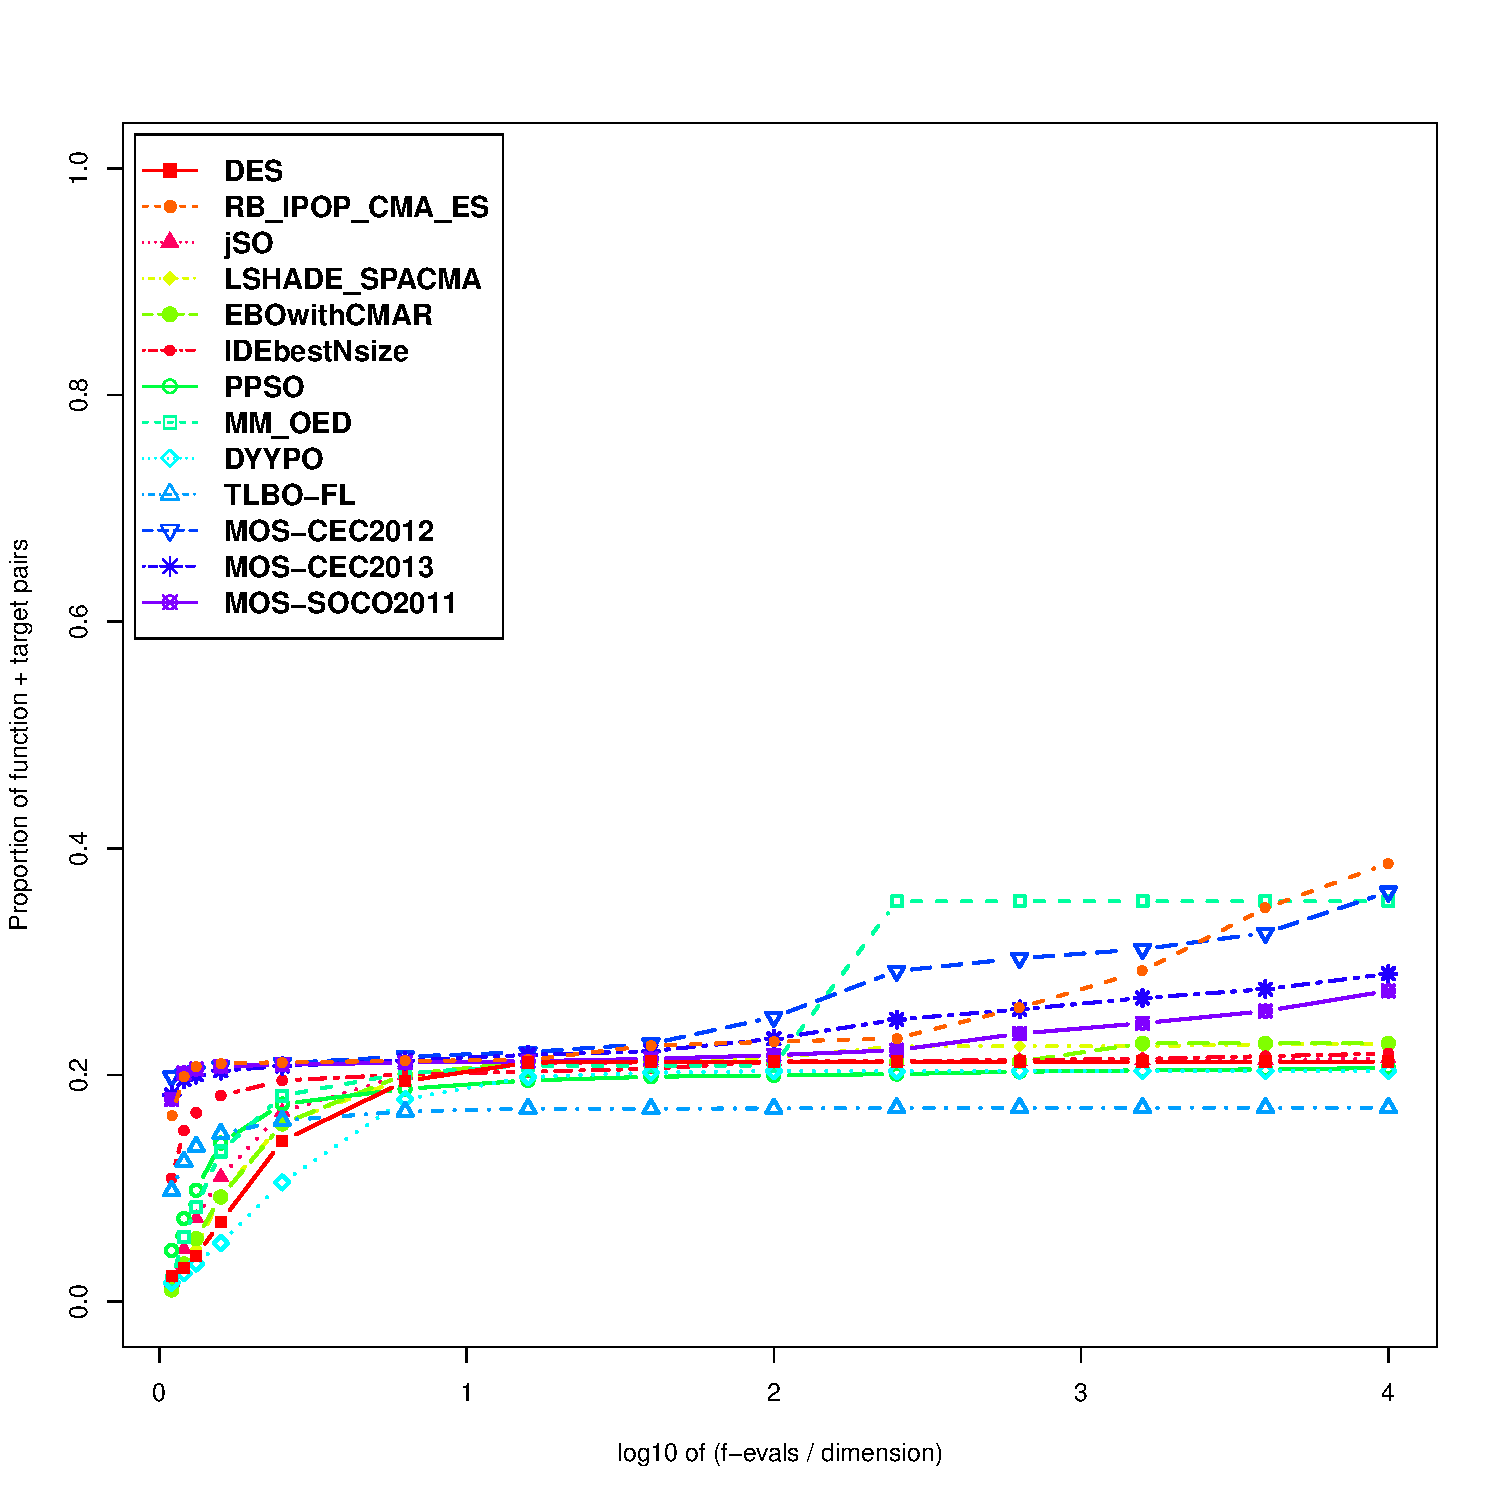
\includegraphics[height=0.9\linewidth,angle=90]{C:/Users/JS/Desktop/Doktorat/EvolutionAlgorithms/IEEEecdf/Plots/singlePlots/Problem=4,N=100.pdf}
    \end{minipage}%
	}   
  \end{subfigure} 
\end{figure}

\end{frame}


\begin{frame}
%\frametitle{CEC2017 Function 5}
\AddToShipoutPictureFG*{
    \AtPageUpperLeft{\put(-135,-12){
    \makebox[\paperwidth][r]{\textcolor{blue}{CEC2017 Function 5}}
    }
    }  
    }%

\begin{figure}[ht] 
    \vspace{-2mm}
\captionsetup[subfigure]{labelformat=empty}
  \begin{subfigure}[b]{0.5\linewidth}
    \centering
      \rotatebox[origin=c]{-90}{
        \begin{minipage}{1\linewidth}
    		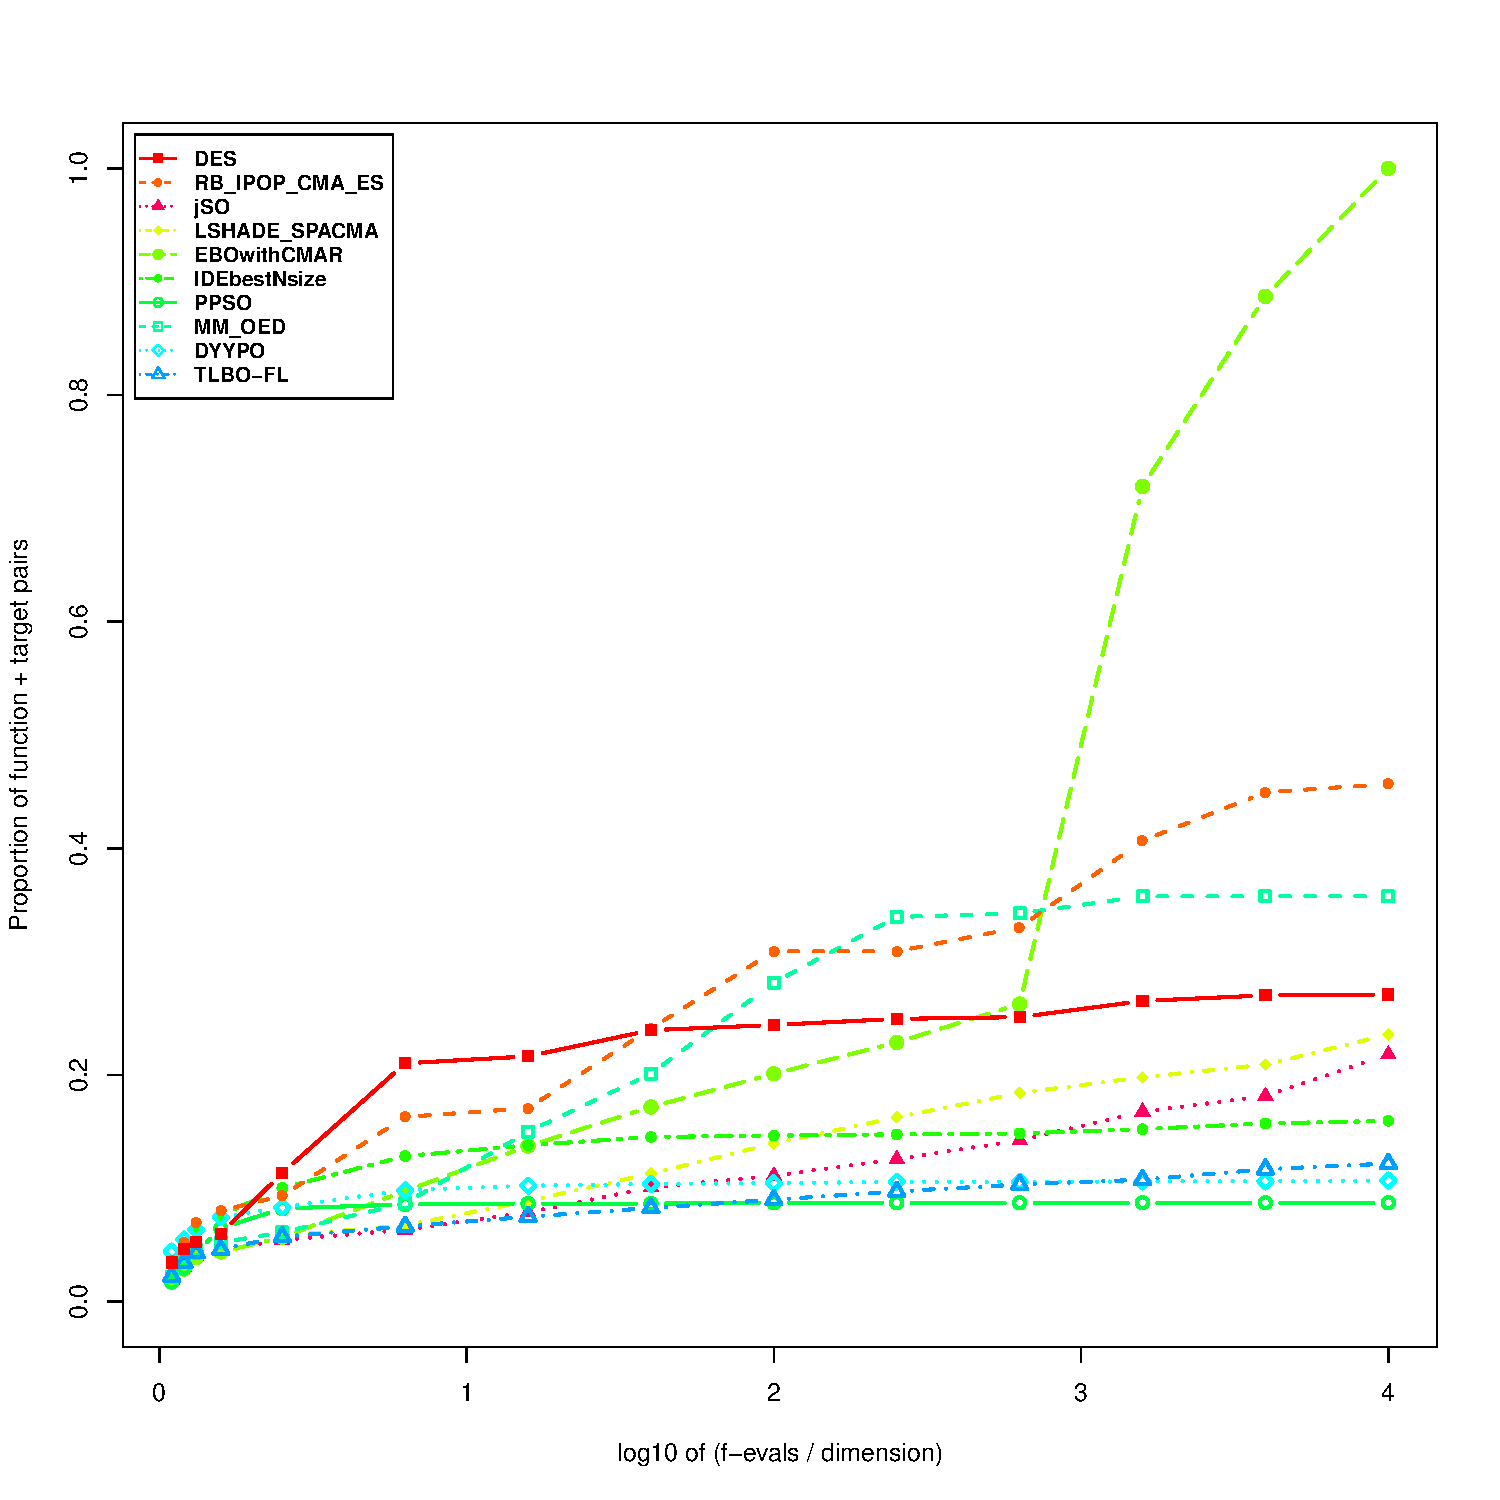
\includegraphics[height=0.9\linewidth,angle=90]{C:/Users/JS/Desktop/Doktorat/EvolutionAlgorithms/IEEEecdf/Plots/singlePlots/Problem=5,N=10.pdf} 
    		\caption{D=10} 
      	\end{minipage}%
	}
    \vspace{-12mm}
  \end{subfigure}%% 
  \begin{subfigure}[b]{0.5\linewidth}
    \centering
    \rotatebox[origin=c]{-90}{
        \begin{minipage}{1\linewidth}
            	\caption{D=30}
    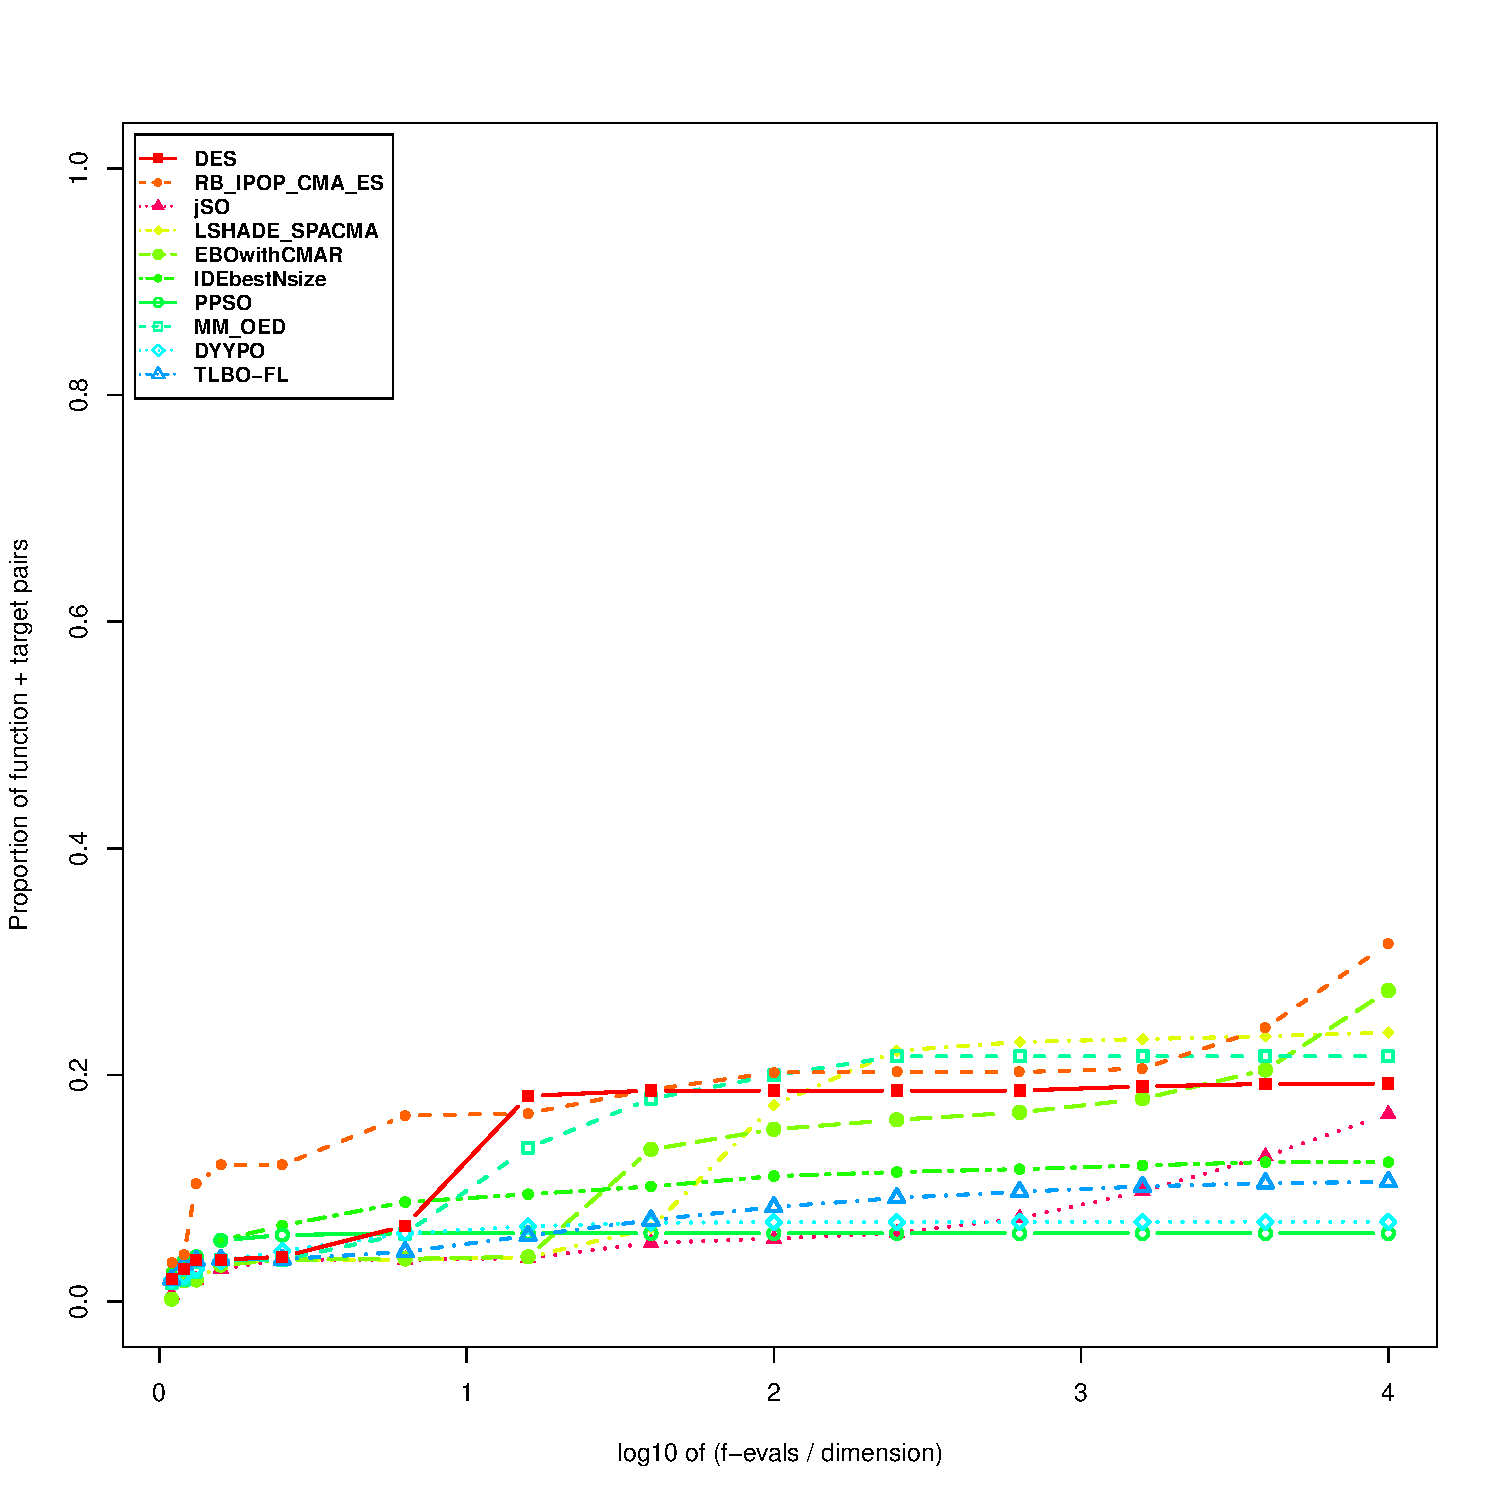
\includegraphics[height=0.9\linewidth,angle=90]{C:/Users/JS/Desktop/Doktorat/EvolutionAlgorithms/IEEEecdf/Plots/singlePlots/Problem=5,N=30.pdf} 
    	\end{minipage}%
	} 
    \vspace{-12mm}
  \end{subfigure} 
  \begin{subfigure}[b]{0.5\linewidth}
    \centering
    \rotatebox[origin=c]{-90}{
        \begin{minipage}{1\linewidth}
    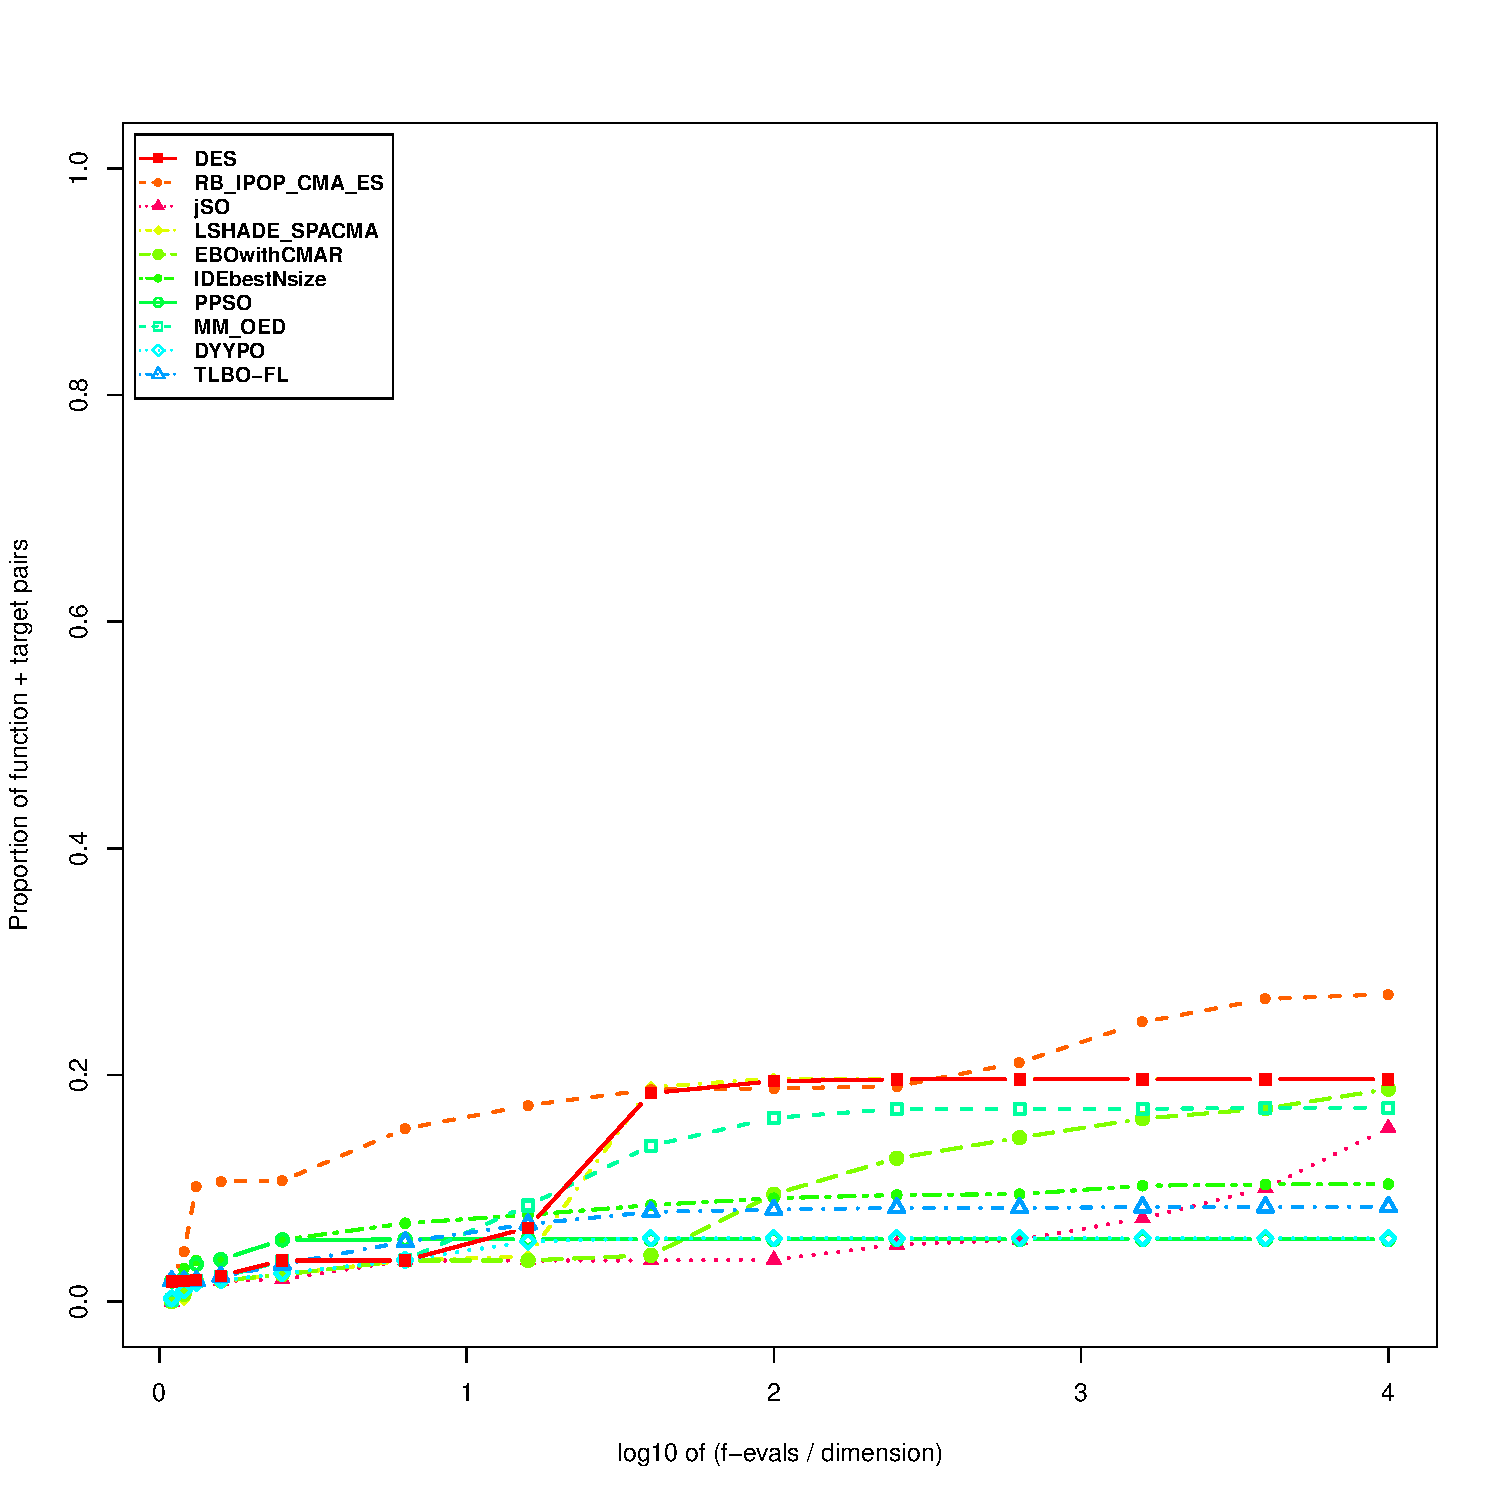
\includegraphics[height=0.9\linewidth,angle=90]{C:/Users/JS/Desktop/Doktorat/EvolutionAlgorithms/IEEEecdf/Plots/singlePlots/Problem=5,N=50.pdf} 
    	\caption{D=50}
    	\end{minipage}%
	}  
  \end{subfigure}%%
  \begin{subfigure}[b]{0.5\linewidth}
    \centering
    \rotatebox[origin=c]{-90}{
        \begin{minipage}{1\linewidth}
        \caption{D=100} 
    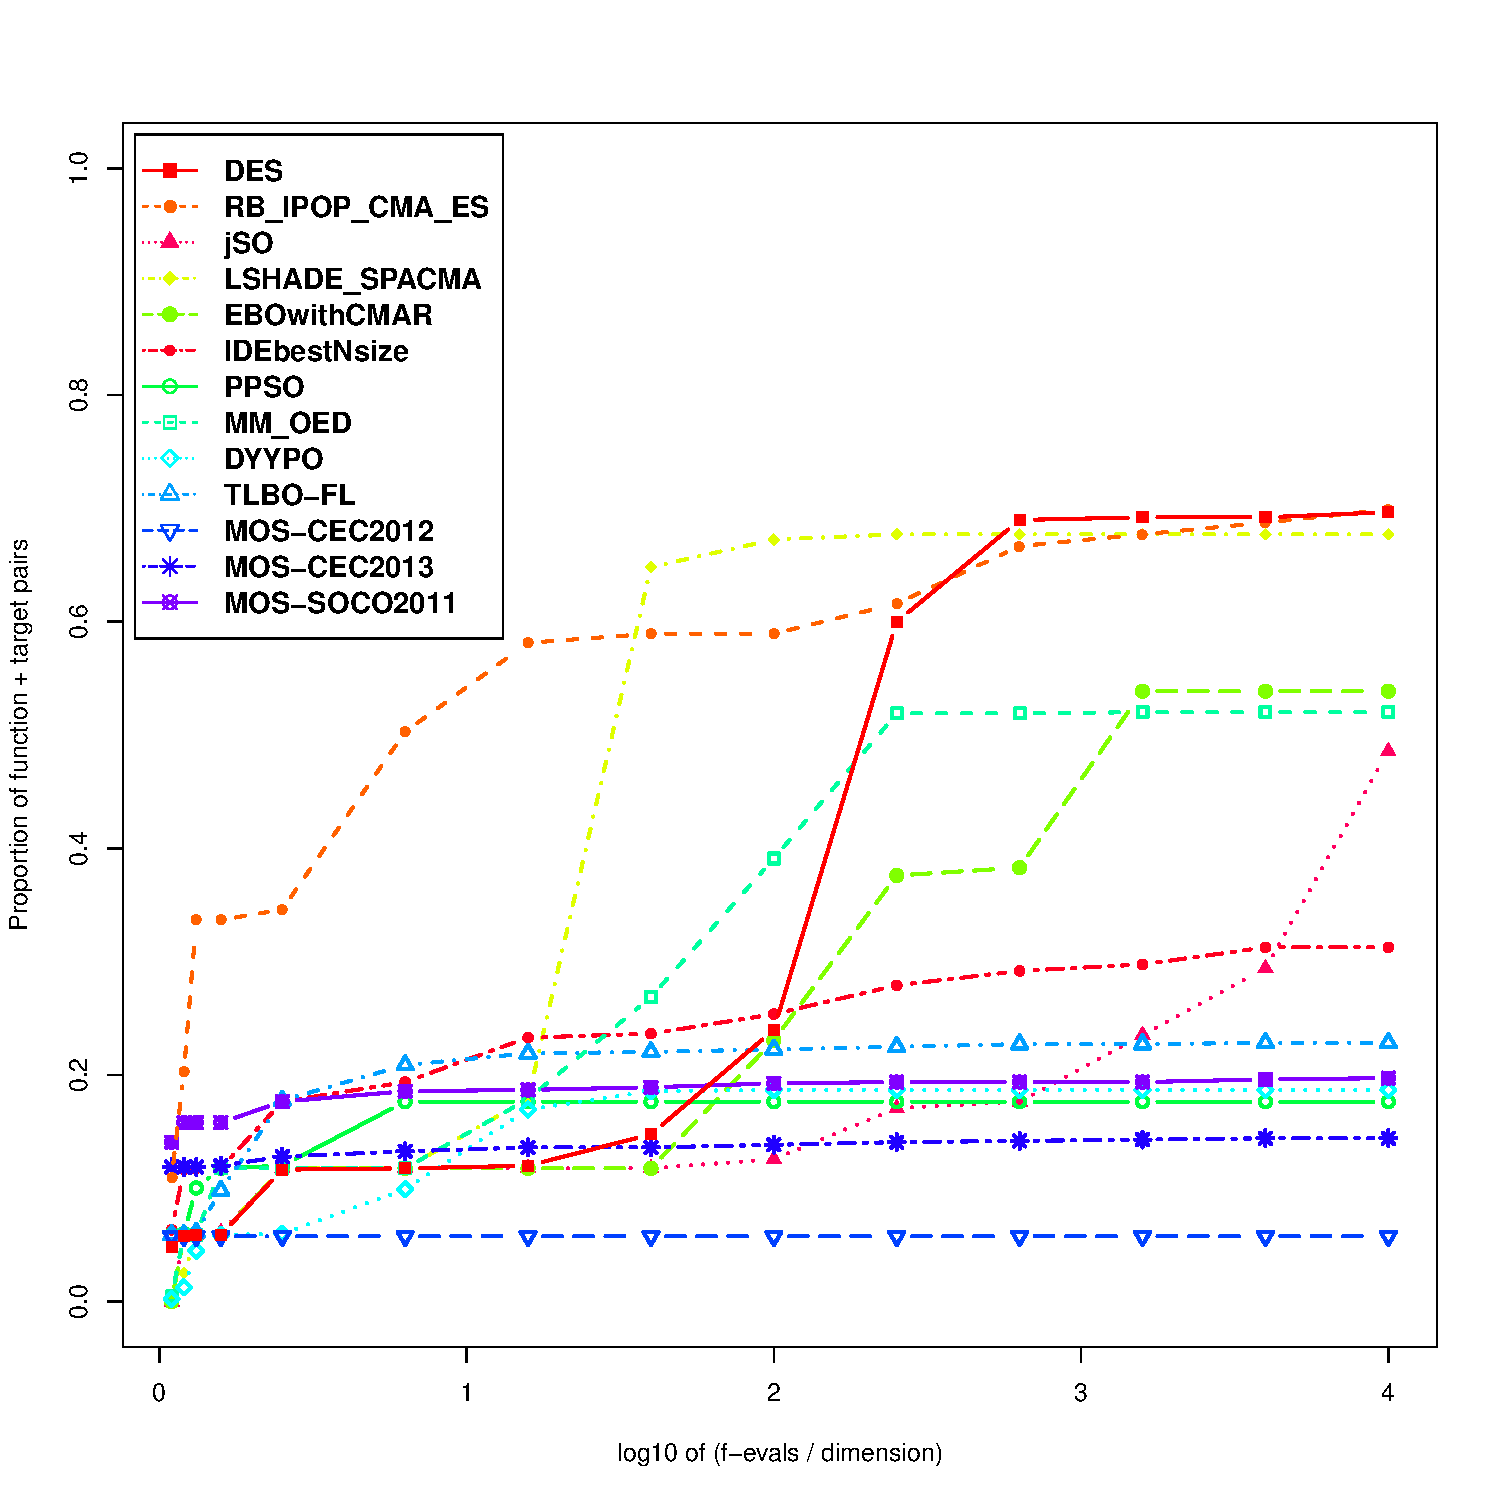
\includegraphics[height=0.9\linewidth,angle=90]{C:/Users/JS/Desktop/Doktorat/EvolutionAlgorithms/IEEEecdf/Plots/singlePlots/Problem=5,N=100.pdf}
    \end{minipage}%
	}   
  \end{subfigure} 
\end{figure}

\end{frame}


\begin{frame}
%\frametitle{CEC2017 Function 6}
\AddToShipoutPictureFG*{
    \AtPageUpperLeft{\put(-135,-12){
    \makebox[\paperwidth][r]{\textcolor{blue}{CEC2017 Function 6}}
    }
    }  
    }%

\begin{figure}[ht] 
    \vspace{-2mm}
\captionsetup[subfigure]{labelformat=empty}
  \begin{subfigure}[b]{0.5\linewidth}
    \centering
      \rotatebox[origin=c]{-90}{
        \begin{minipage}{1\linewidth}
    		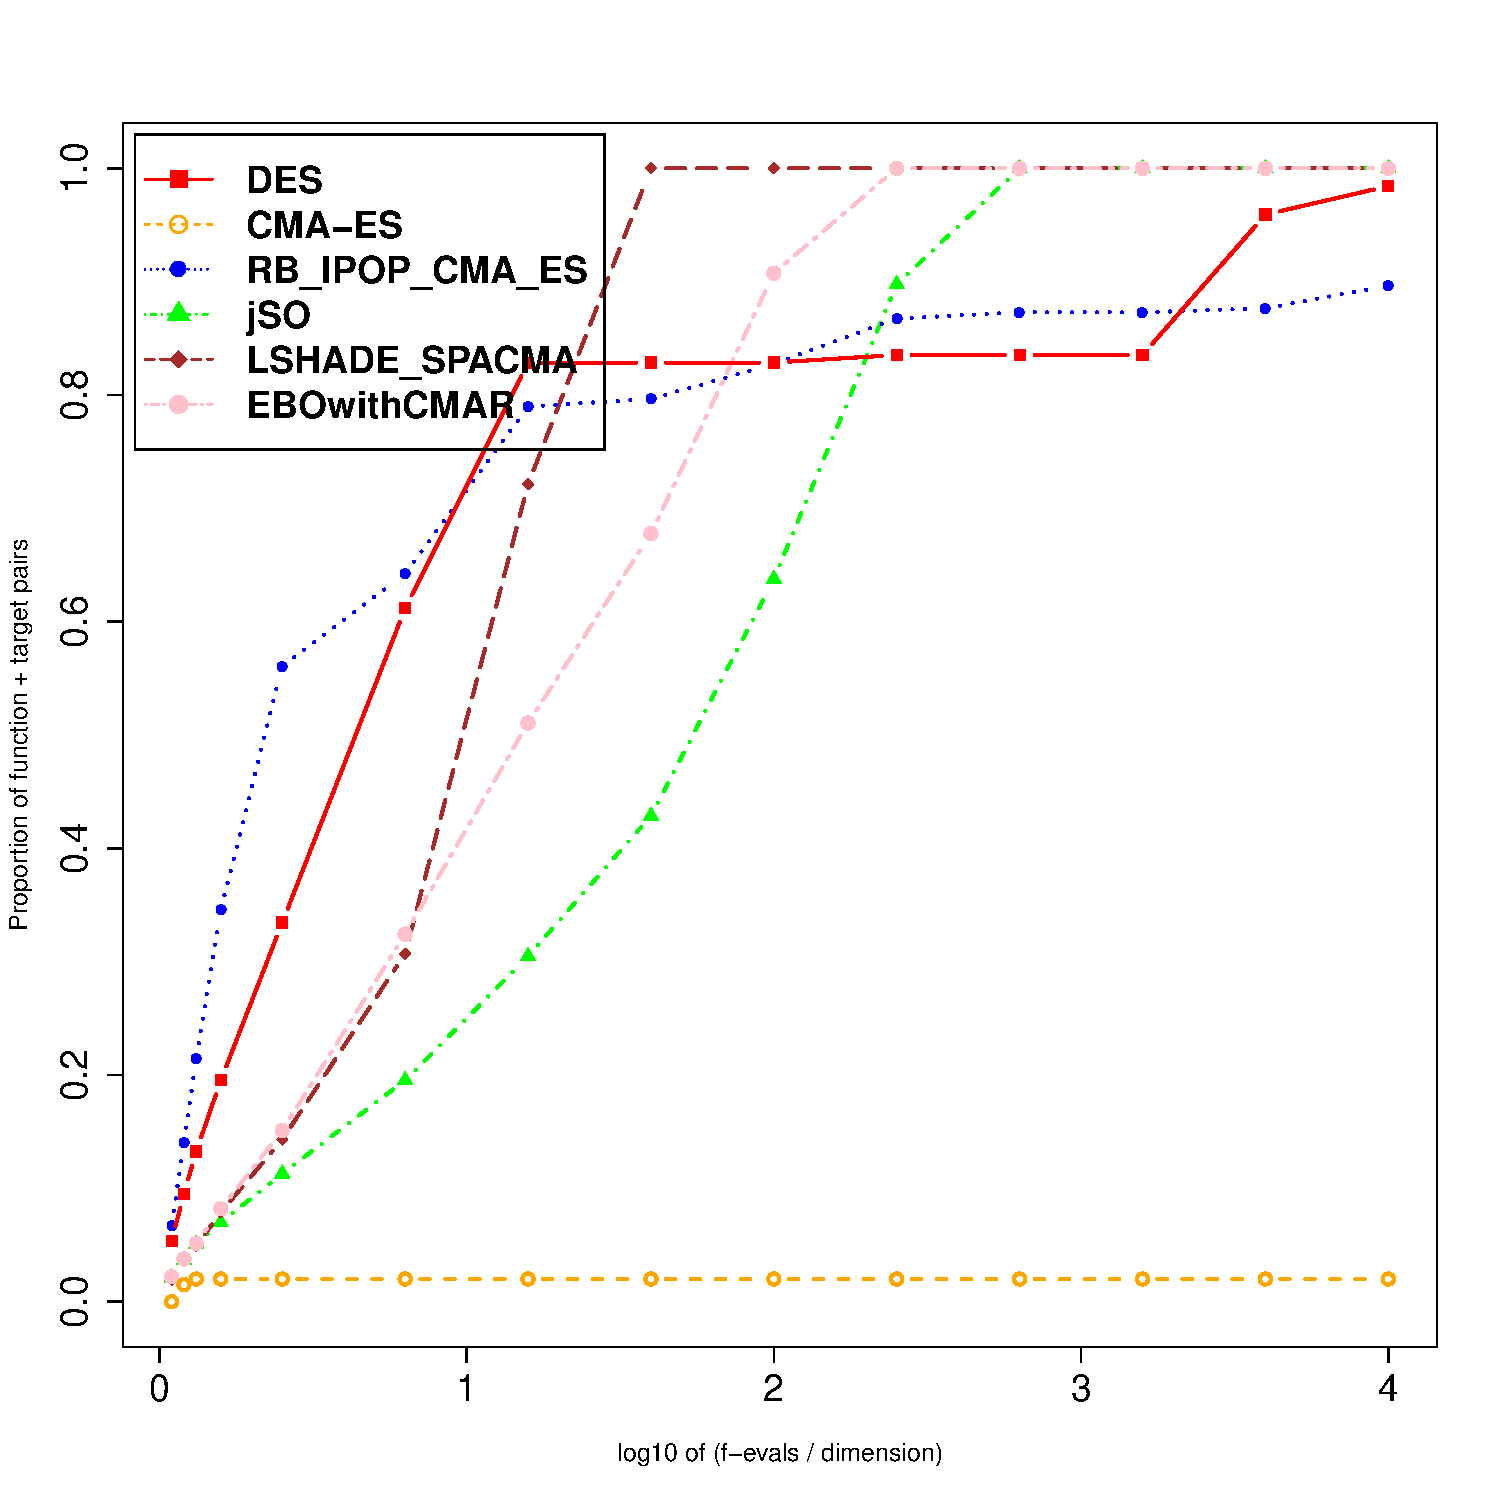
\includegraphics[height=0.9\linewidth,angle=90]{C:/Users/JS/Desktop/Doktorat/EvolutionAlgorithms/IEEEecdf/Plots/singlePlots/Problem=6,N=10.pdf} 
    		\caption{D=10} 
      	\end{minipage}%
	}
    \vspace{-12mm}
  \end{subfigure}%% 
  \begin{subfigure}[b]{0.5\linewidth}
    \centering
    \rotatebox[origin=c]{-90}{
        \begin{minipage}{1\linewidth}
            	\caption{D=30}
    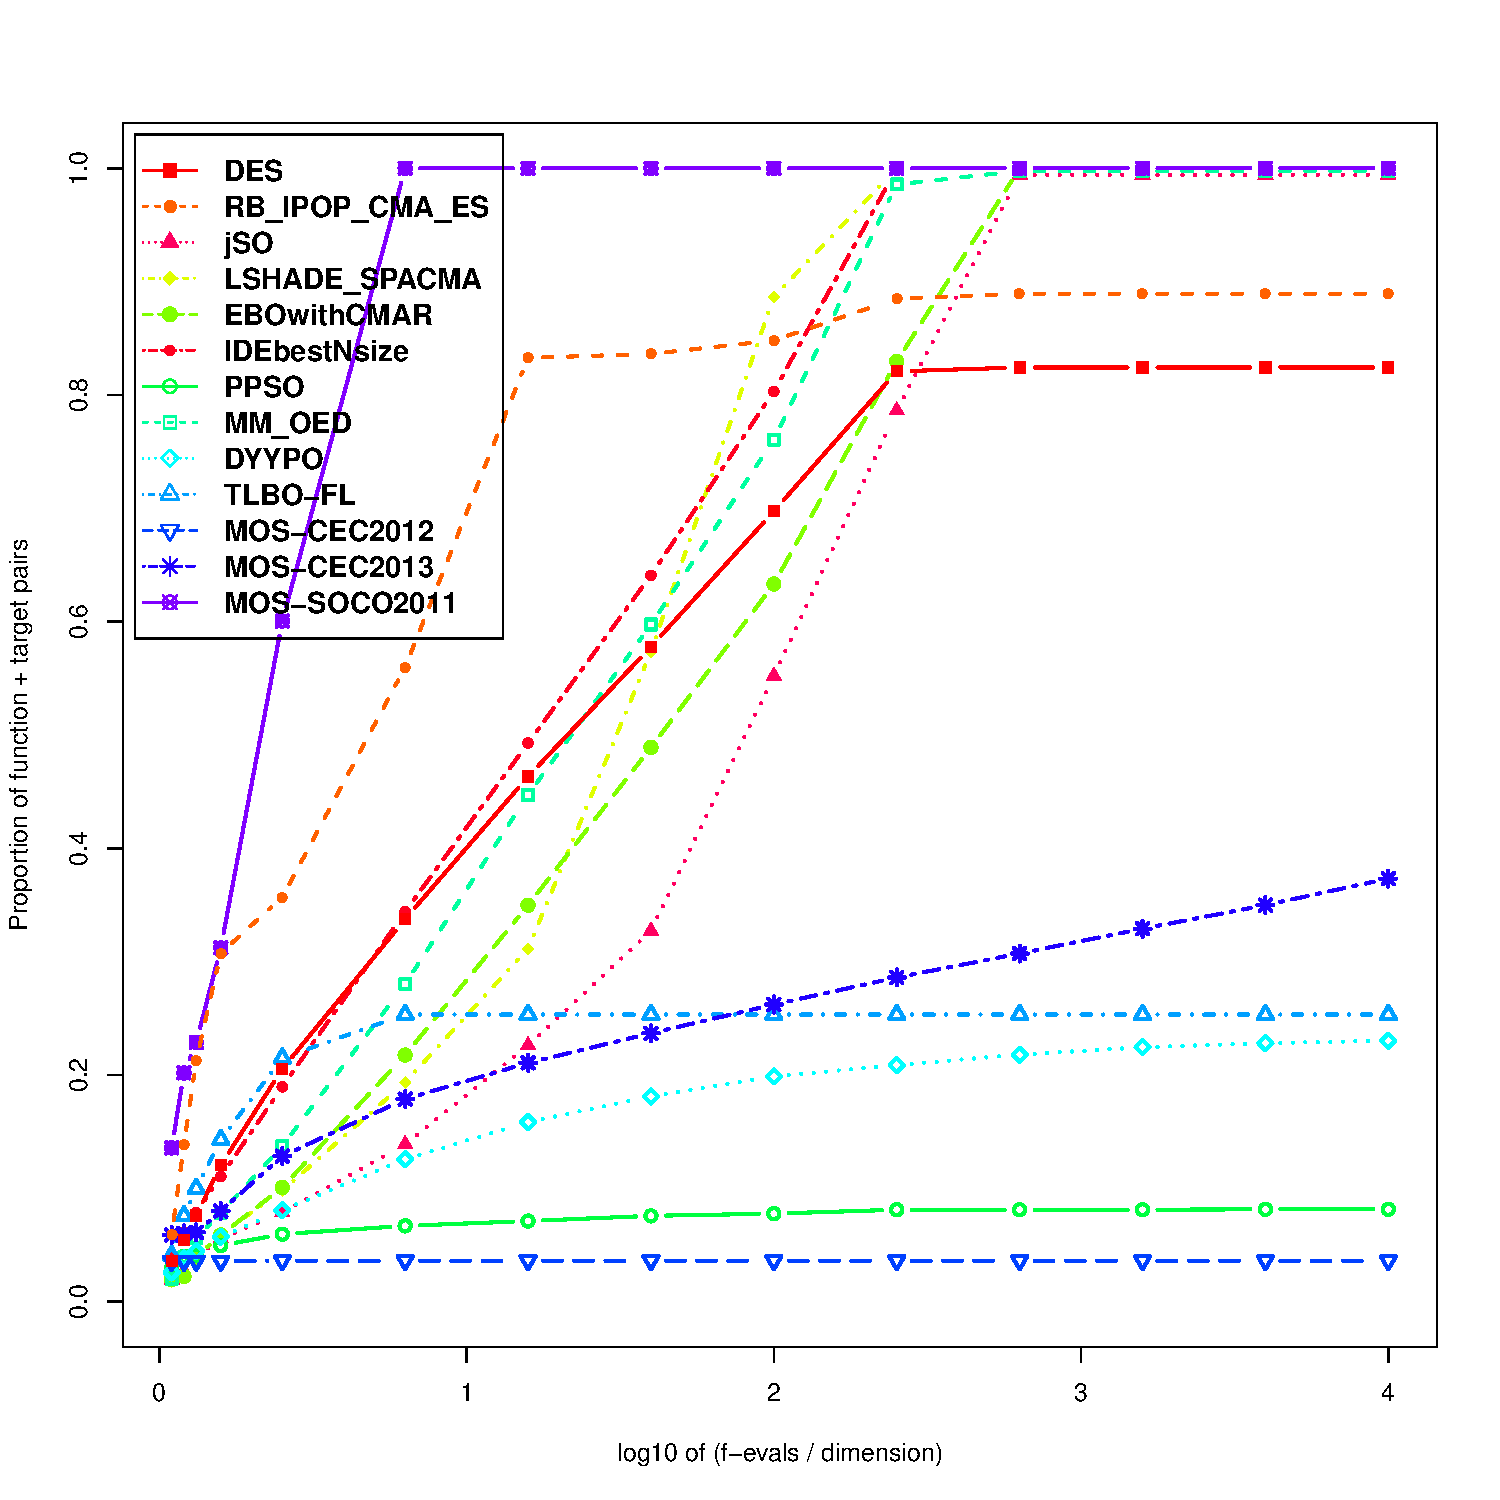
\includegraphics[height=0.9\linewidth,angle=90]{C:/Users/JS/Desktop/Doktorat/EvolutionAlgorithms/IEEEecdf/Plots/singlePlots/Problem=6,N=30.pdf} 
    	\end{minipage}%
	} 
    \vspace{-12mm}
  \end{subfigure} 
  \begin{subfigure}[b]{0.5\linewidth}
    \centering
    \rotatebox[origin=c]{-90}{
        \begin{minipage}{1\linewidth}
    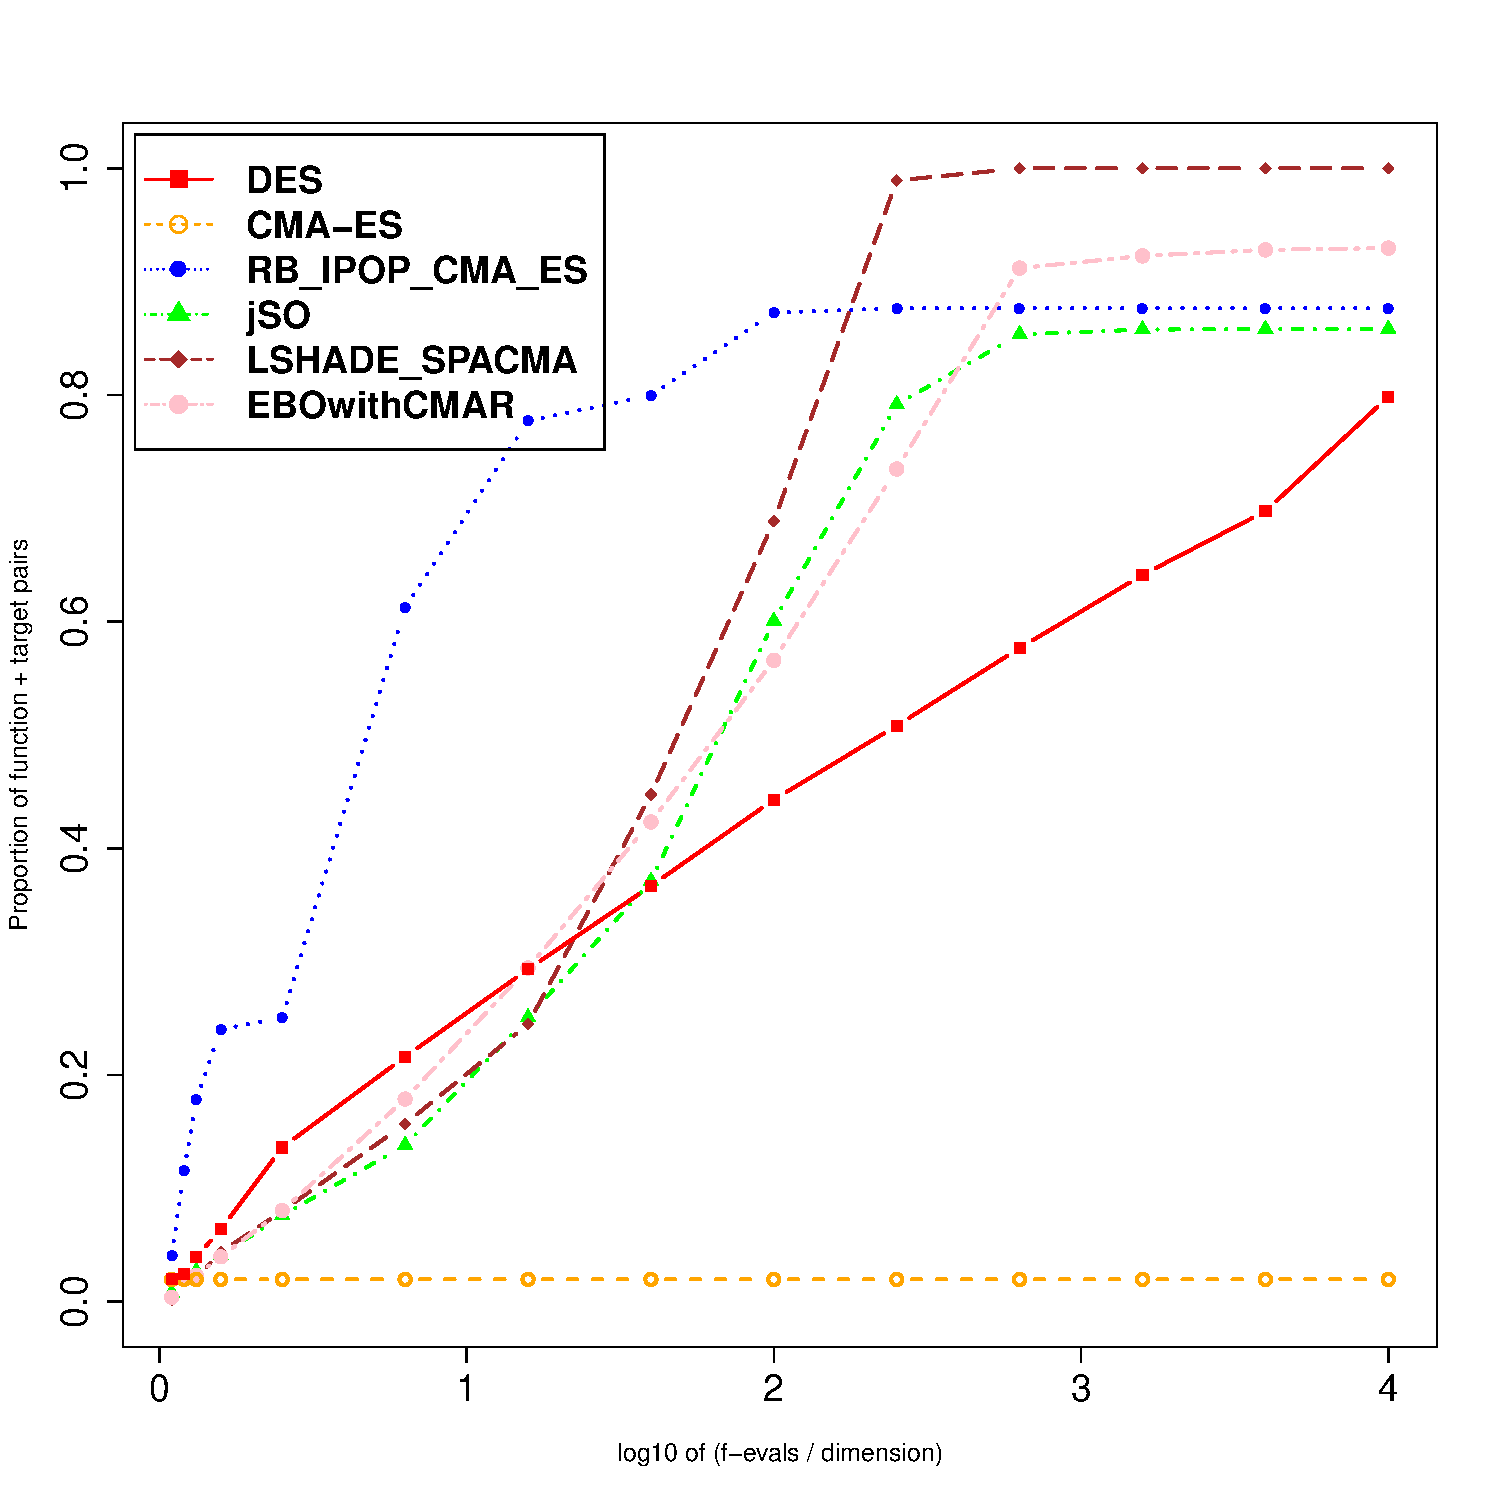
\includegraphics[height=0.9\linewidth,angle=90]{C:/Users/JS/Desktop/Doktorat/EvolutionAlgorithms/IEEEecdf/Plots/singlePlots/Problem=6,N=50.pdf} 
    	\caption{D=50}
    	\end{minipage}%
	}  
  \end{subfigure}%%
  \begin{subfigure}[b]{0.5\linewidth}
    \centering
    \rotatebox[origin=c]{-90}{
        \begin{minipage}{1\linewidth}
        \caption{D=100} 
    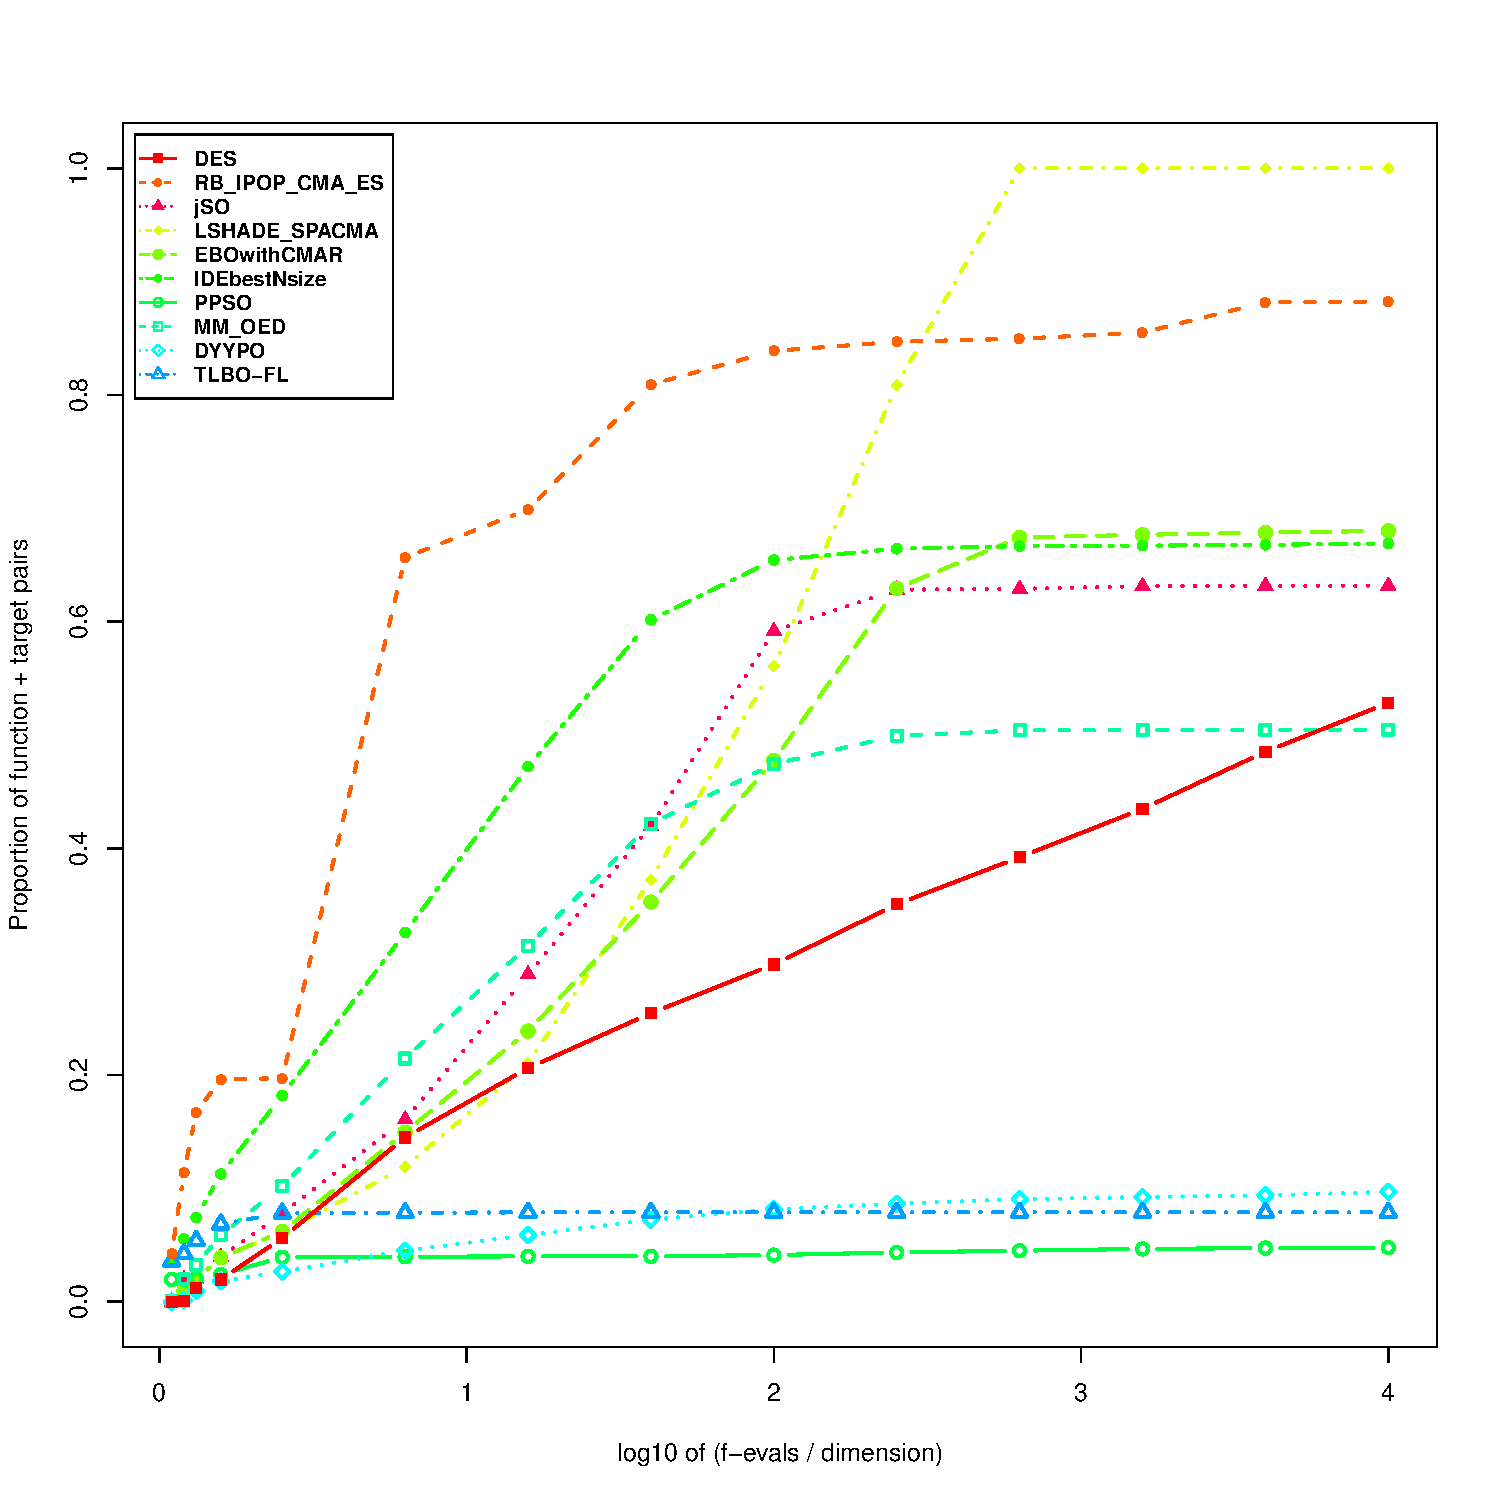
\includegraphics[height=0.9\linewidth,angle=90]{C:/Users/JS/Desktop/Doktorat/EvolutionAlgorithms/IEEEecdf/Plots/singlePlots/Problem=6,N=100.pdf}
    \end{minipage}%
	}   
  \end{subfigure} 
\end{figure}

\end{frame}


\begin{frame}
%\frametitle{CEC2017 Function 7}
\AddToShipoutPictureFG*{
    \AtPageUpperLeft{\put(-135,-12){
    \makebox[\paperwidth][r]{\textcolor{blue}{CEC2017 Function 7}}
    }
    }  
    }%

\begin{figure}[ht] 
    \vspace{-2mm}
\captionsetup[subfigure]{labelformat=empty}
  \begin{subfigure}[b]{0.5\linewidth}
    \centering
      \rotatebox[origin=c]{-90}{
        \begin{minipage}{1\linewidth}
    		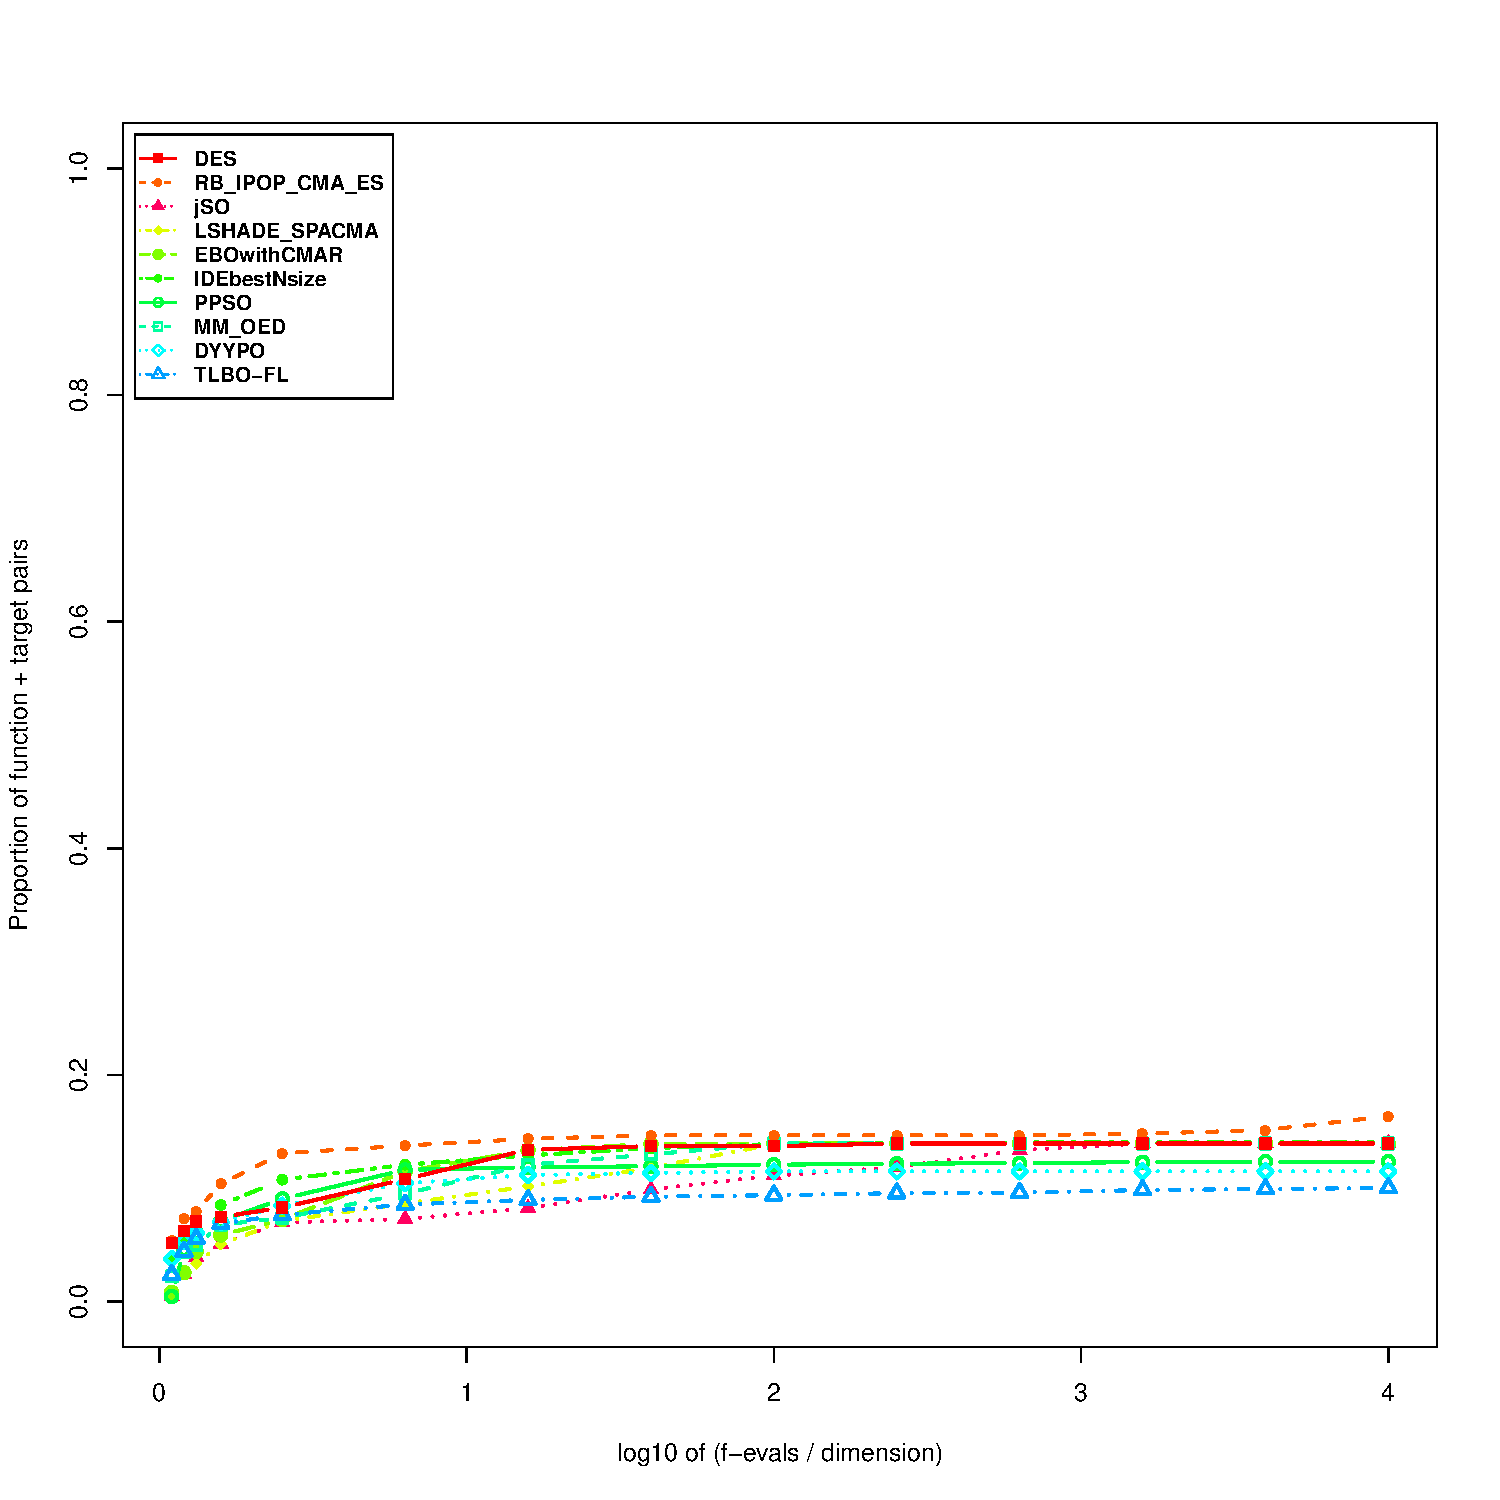
\includegraphics[height=0.9\linewidth,angle=90]{C:/Users/JS/Desktop/Doktorat/EvolutionAlgorithms/IEEEecdf/Plots/singlePlots/Problem=7,N=10.pdf} 
    		\caption{D=10} 
      	\end{minipage}%
	}
    \vspace{-12mm}
  \end{subfigure}%% 
  \begin{subfigure}[b]{0.5\linewidth}
    \centering
    \rotatebox[origin=c]{-90}{
        \begin{minipage}{1\linewidth}
            	\caption{D=30}
    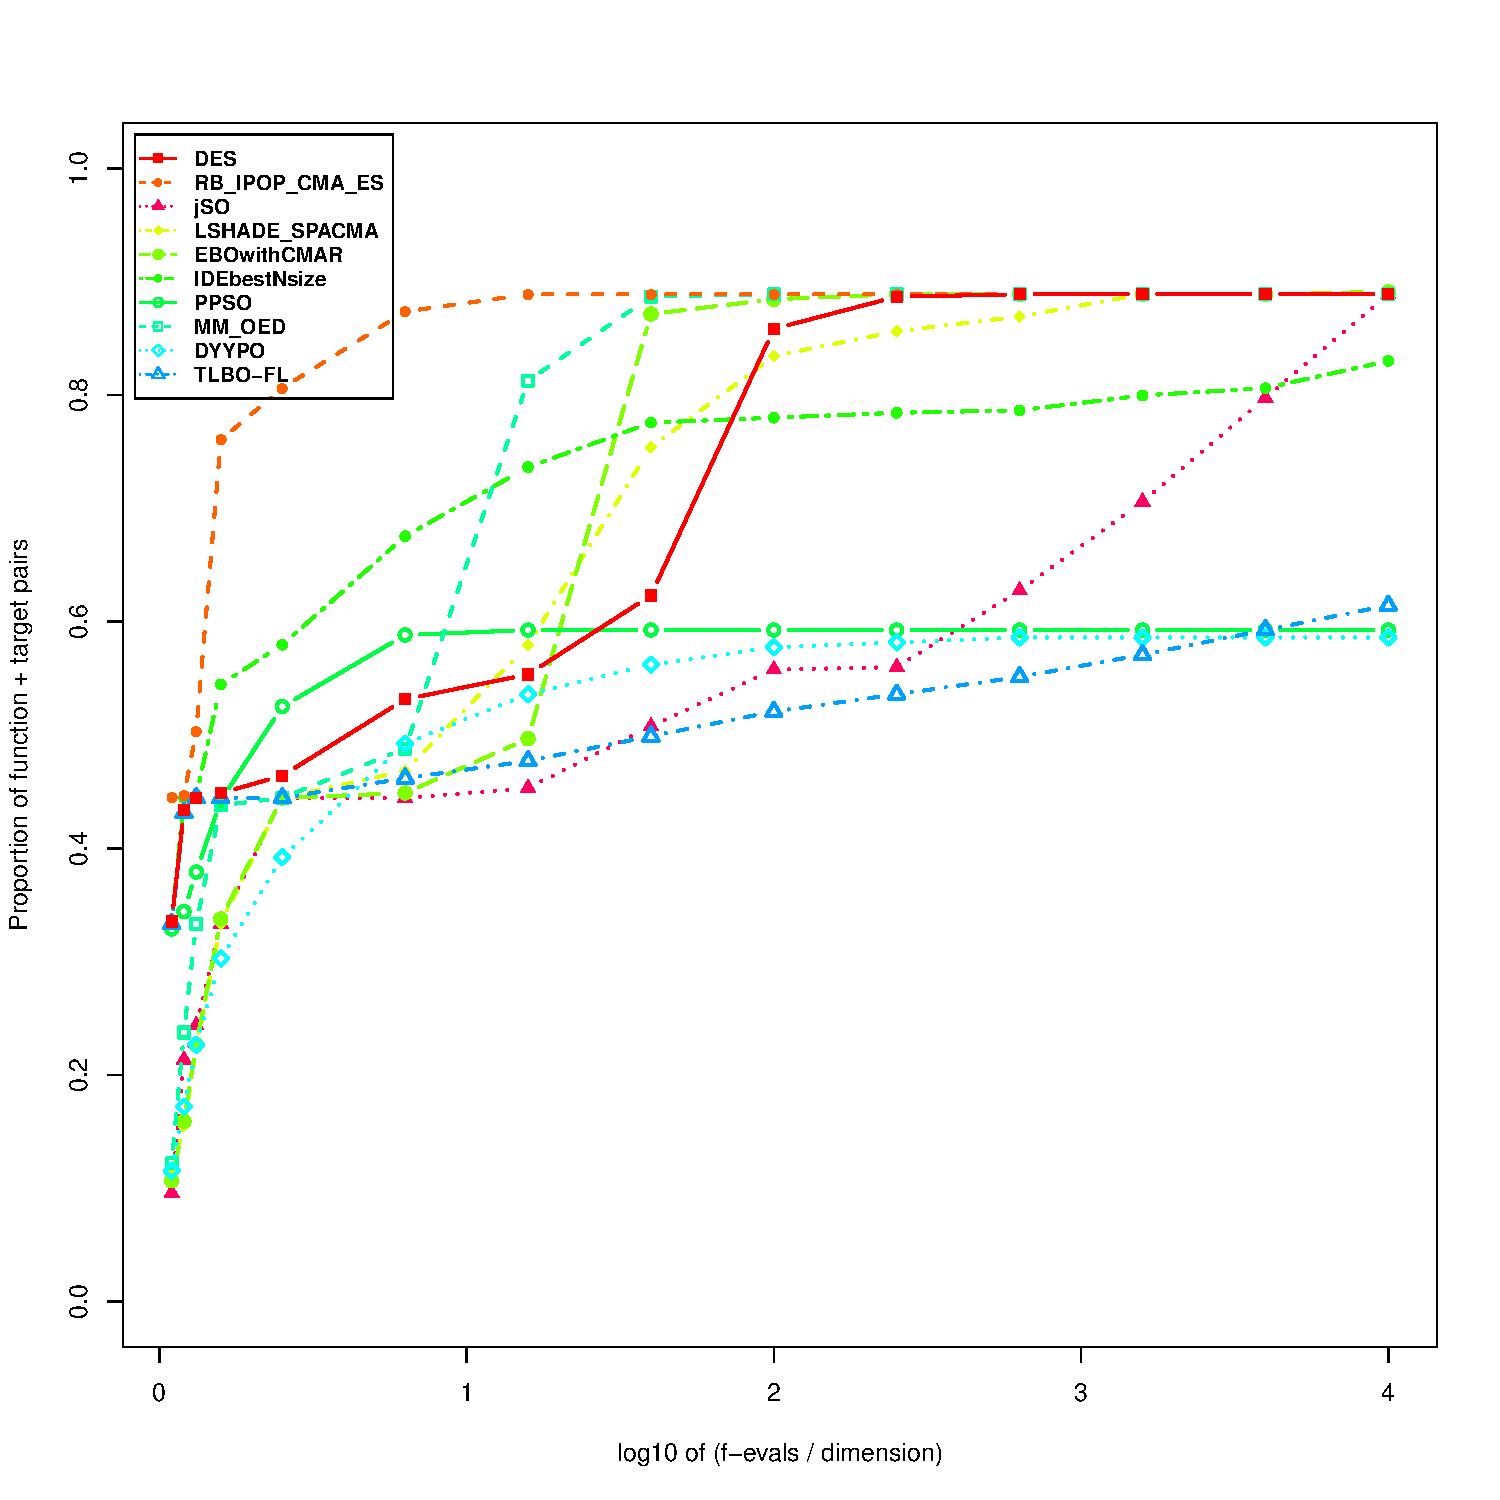
\includegraphics[height=0.9\linewidth,angle=90]{C:/Users/JS/Desktop/Doktorat/EvolutionAlgorithms/IEEEecdf/Plots/singlePlots/Problem=7,N=30.pdf} 
    	\end{minipage}%
	} 
    \vspace{-12mm}
  \end{subfigure} 
  \begin{subfigure}[b]{0.5\linewidth}
    \centering
    \rotatebox[origin=c]{-90}{
        \begin{minipage}{1\linewidth}
    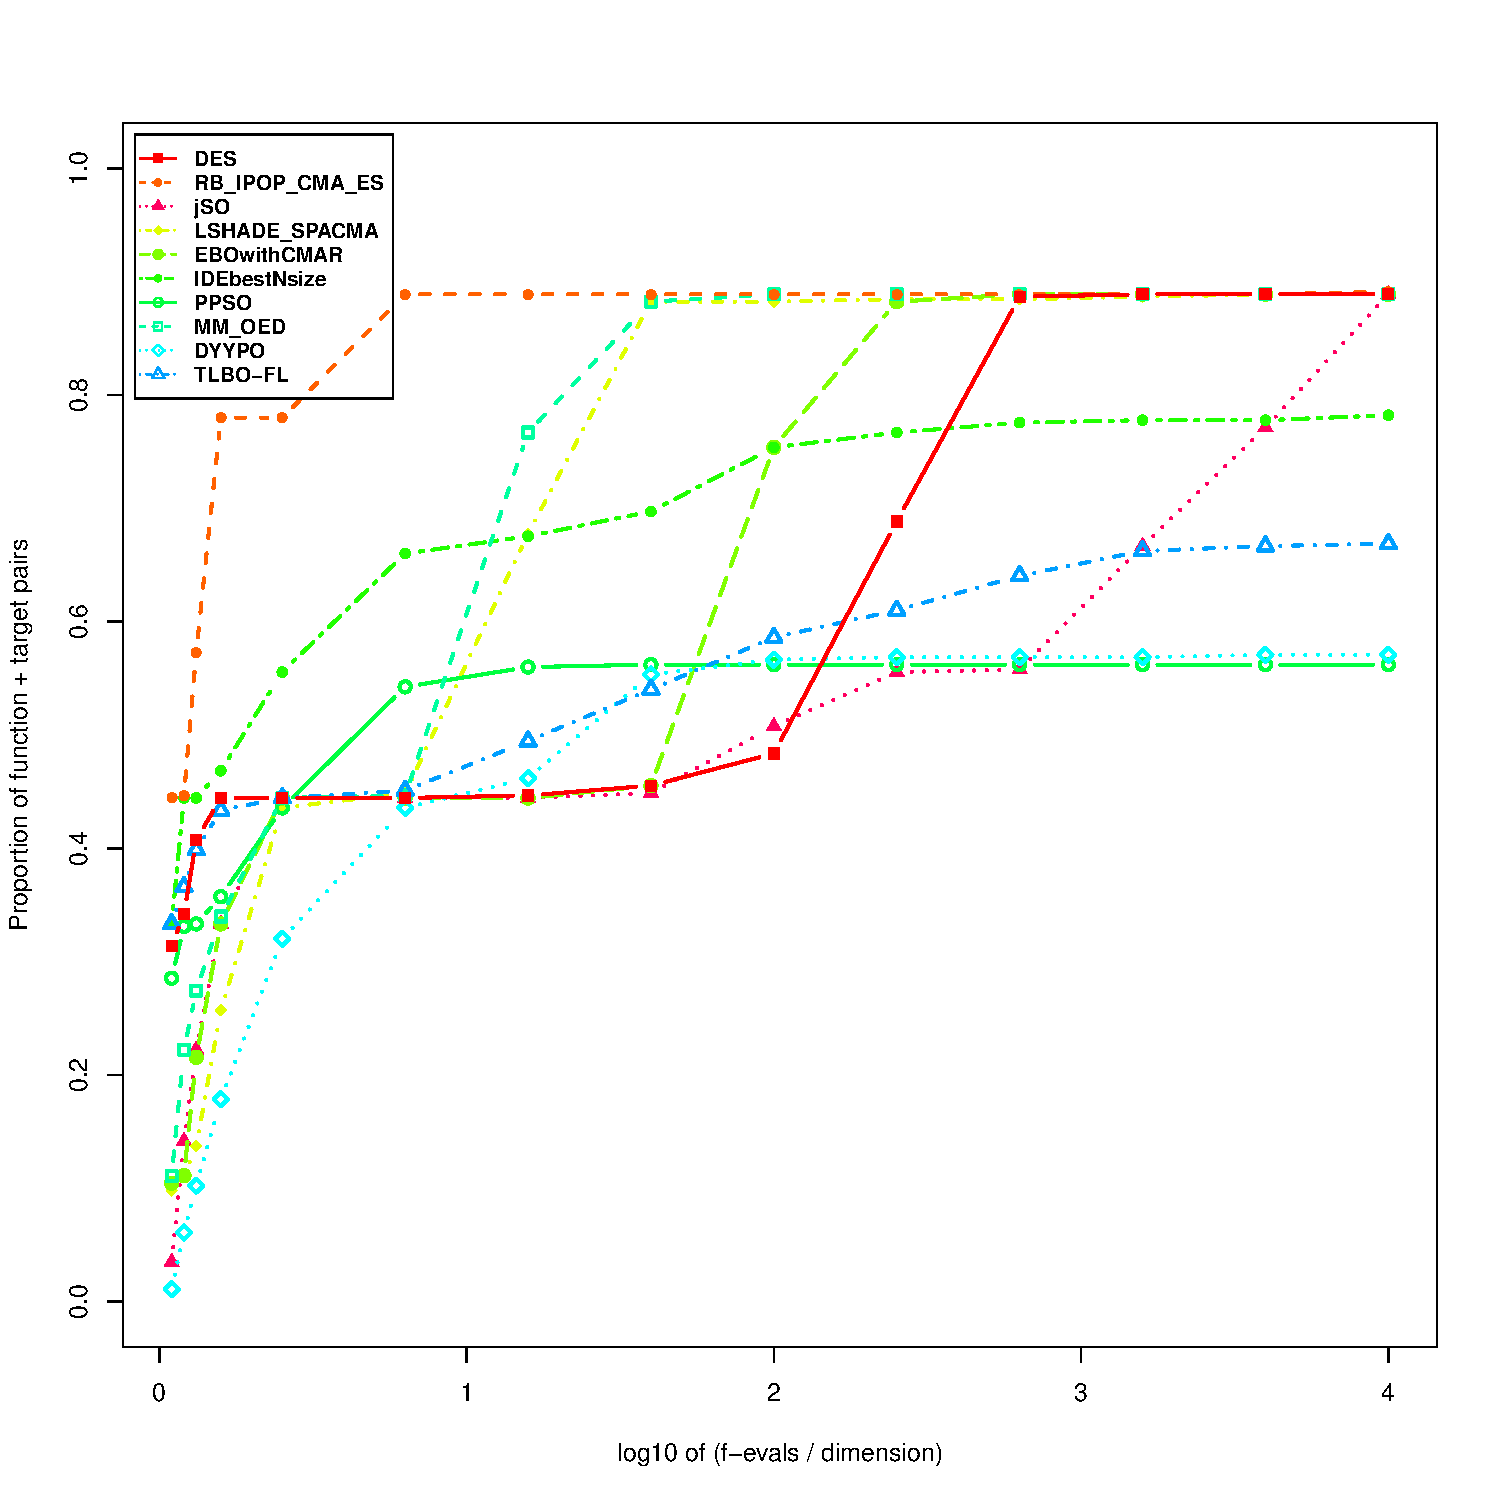
\includegraphics[height=0.9\linewidth,angle=90]{C:/Users/JS/Desktop/Doktorat/EvolutionAlgorithms/IEEEecdf/Plots/singlePlots/Problem=7,N=50.pdf} 
    	\caption{D=50}
    	\end{minipage}%
	}  
  \end{subfigure}%%
  \begin{subfigure}[b]{0.5\linewidth}
    \centering
    \rotatebox[origin=c]{-90}{
        \begin{minipage}{1\linewidth}
        \caption{D=100} 
    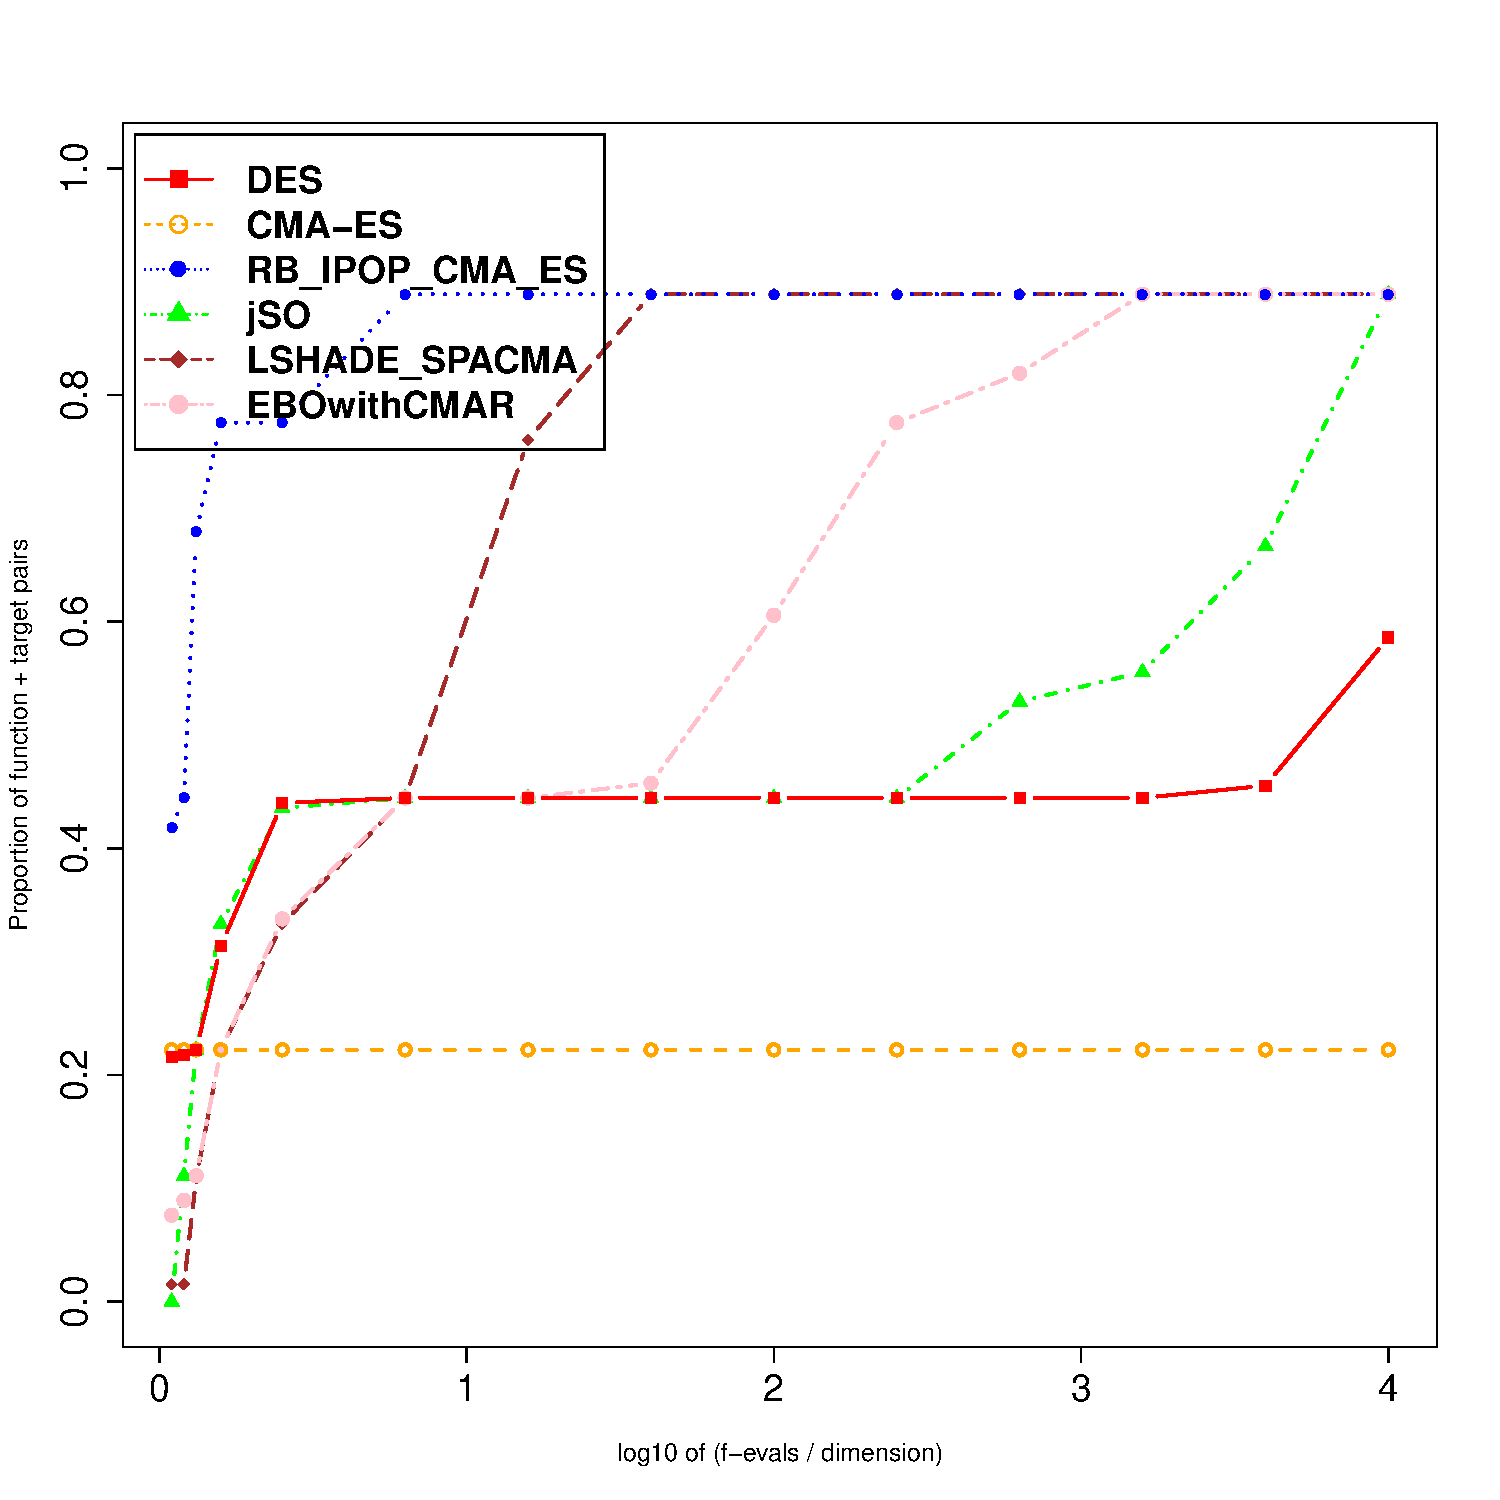
\includegraphics[height=0.9\linewidth,angle=90]{C:/Users/JS/Desktop/Doktorat/EvolutionAlgorithms/IEEEecdf/Plots/singlePlots/Problem=7,N=100.pdf}
    \end{minipage}%
	}   
  \end{subfigure} 
\end{figure}

\end{frame}



\begin{frame}
%\frametitle{CEC2017 Function 8}
\AddToShipoutPictureFG*{
    \AtPageUpperLeft{\put(-135,-12){
    \makebox[\paperwidth][r]{\textcolor{blue}{CEC2017 Function 8}}
    }
    }  
    }%

\begin{figure}[ht] 
    \vspace{-2mm}
\captionsetup[subfigure]{labelformat=empty}
  \begin{subfigure}[b]{0.5\linewidth}
    \centering
      \rotatebox[origin=c]{-90}{
        \begin{minipage}{1\linewidth}
    		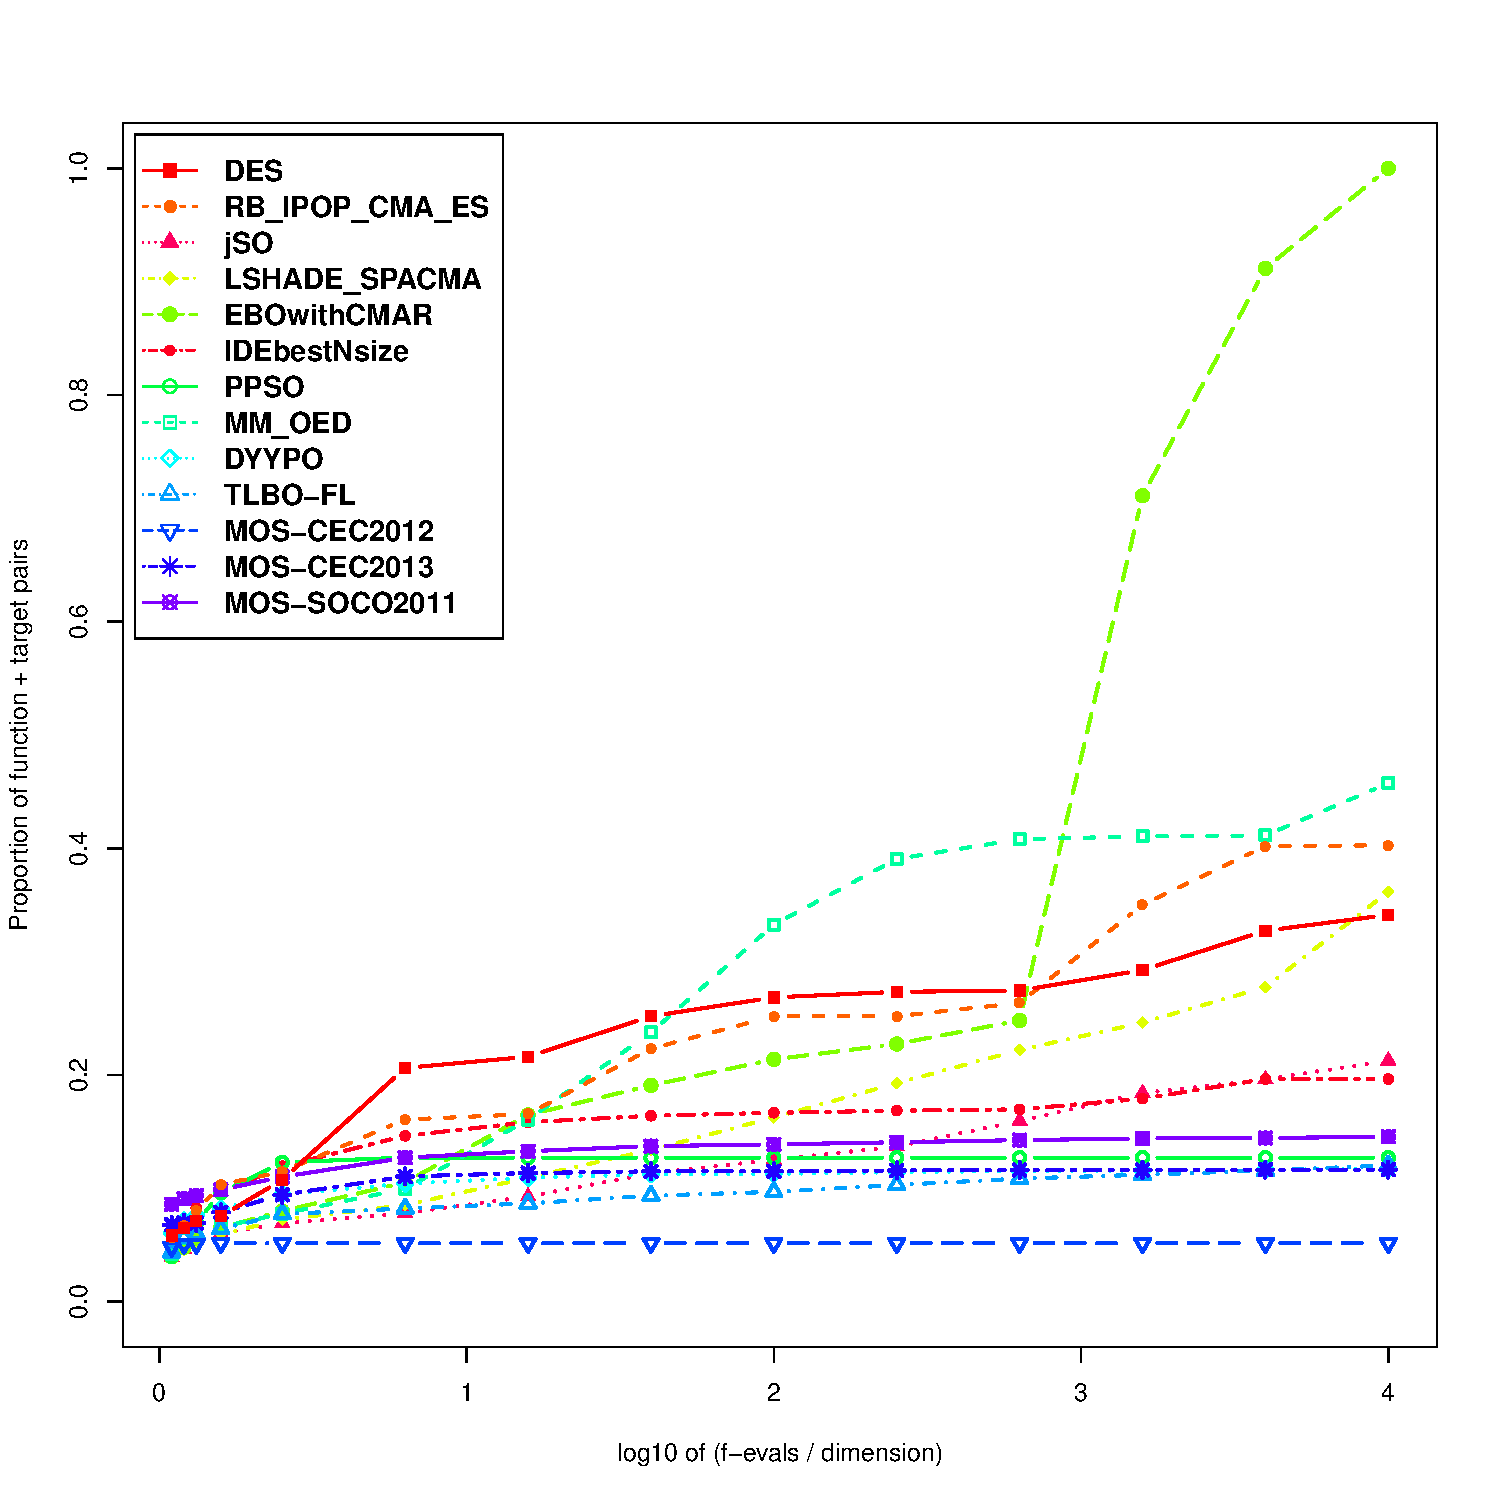
\includegraphics[height=0.9\linewidth,angle=90]{C:/Users/JS/Desktop/Doktorat/EvolutionAlgorithms/IEEEecdf/Plots/singlePlots/Problem=8,N=10.pdf} 
    		\caption{D=10} 
      	\end{minipage}%
	}
    \vspace{-12mm}
  \end{subfigure}%% 
  \begin{subfigure}[b]{0.5\linewidth}
    \centering
    \rotatebox[origin=c]{-90}{
        \begin{minipage}{1\linewidth}
            	\caption{D=30}
    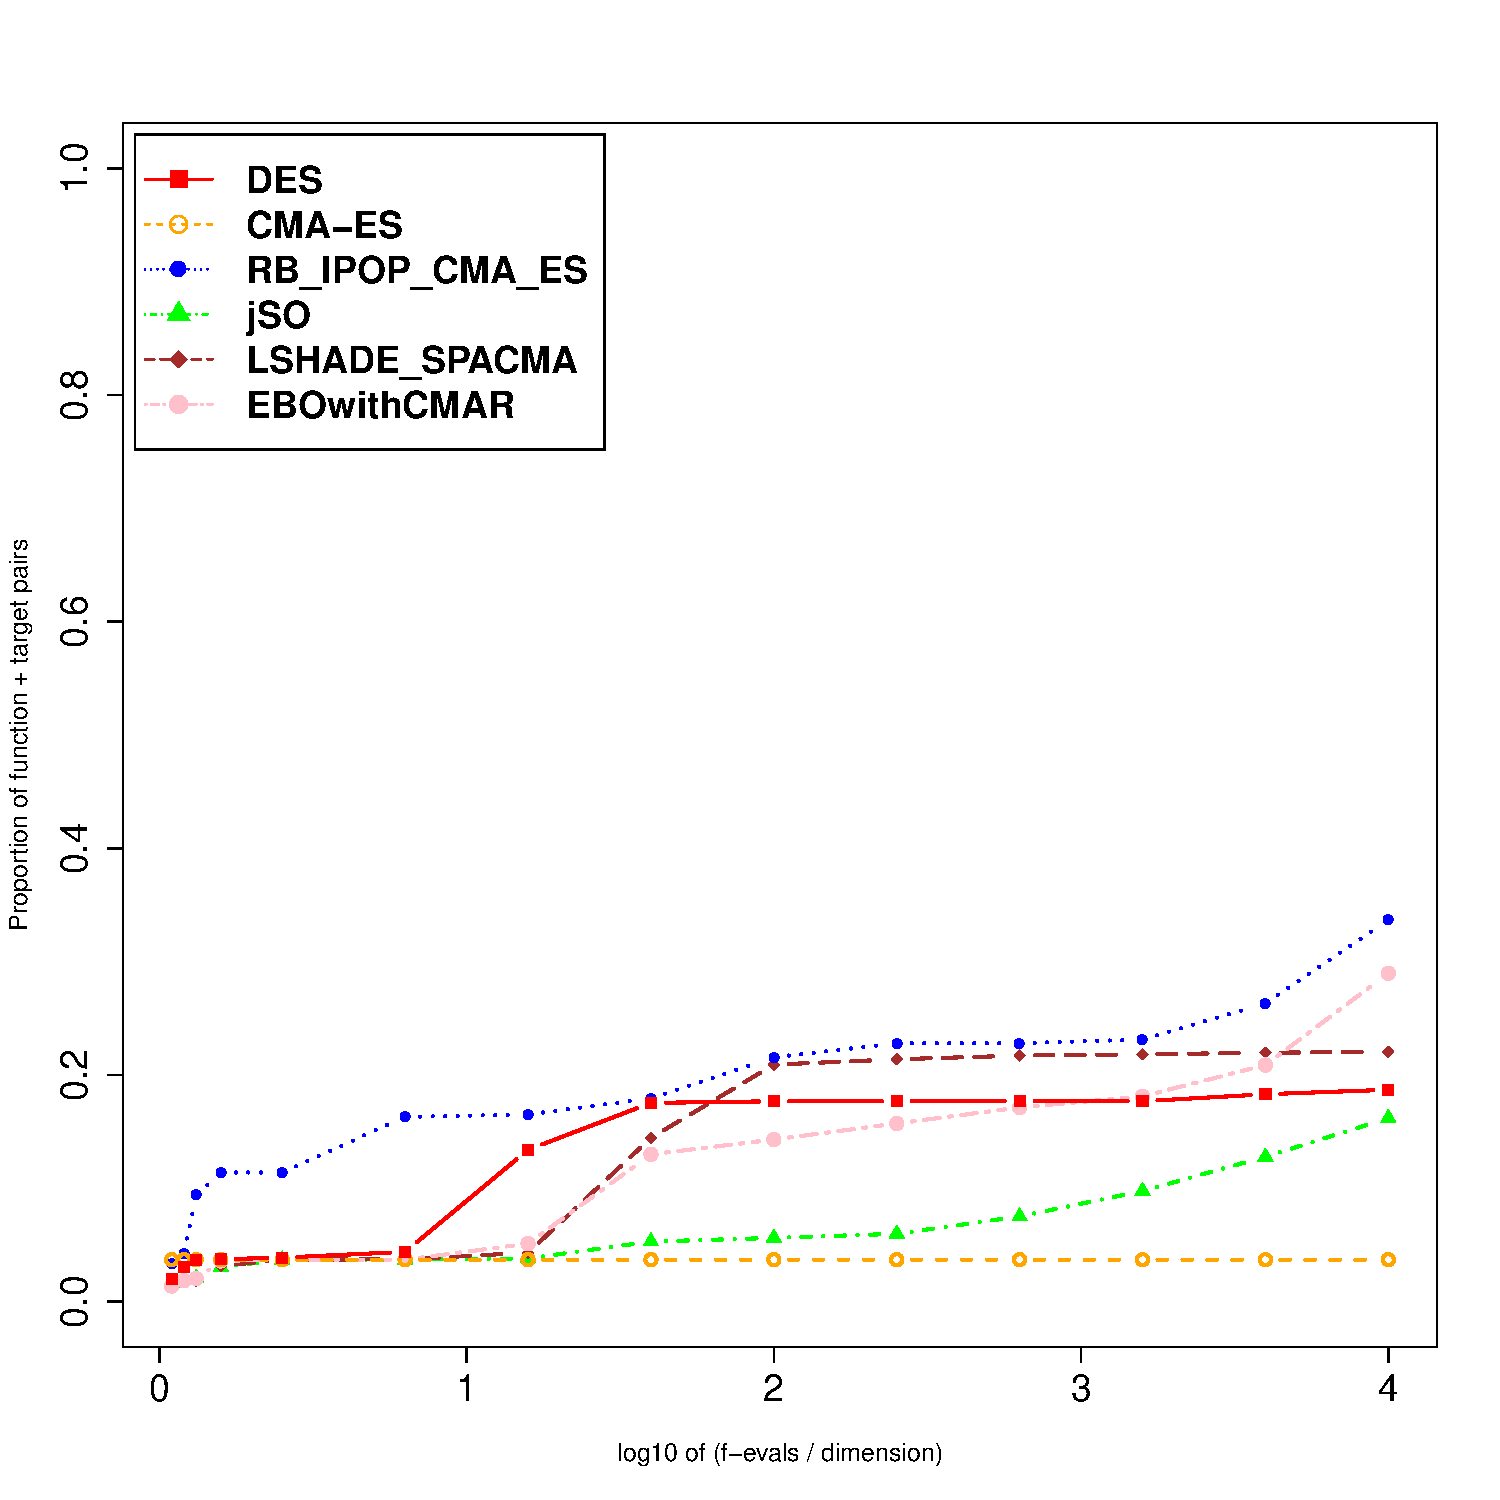
\includegraphics[height=0.9\linewidth,angle=90]{C:/Users/JS/Desktop/Doktorat/EvolutionAlgorithms/IEEEecdf/Plots/singlePlots/Problem=8,N=30.pdf} 
    	\end{minipage}%
	} 
    \vspace{-12mm}
  \end{subfigure} 
  \begin{subfigure}[b]{0.5\linewidth}
    \centering
    \rotatebox[origin=c]{-90}{
        \begin{minipage}{1\linewidth}
    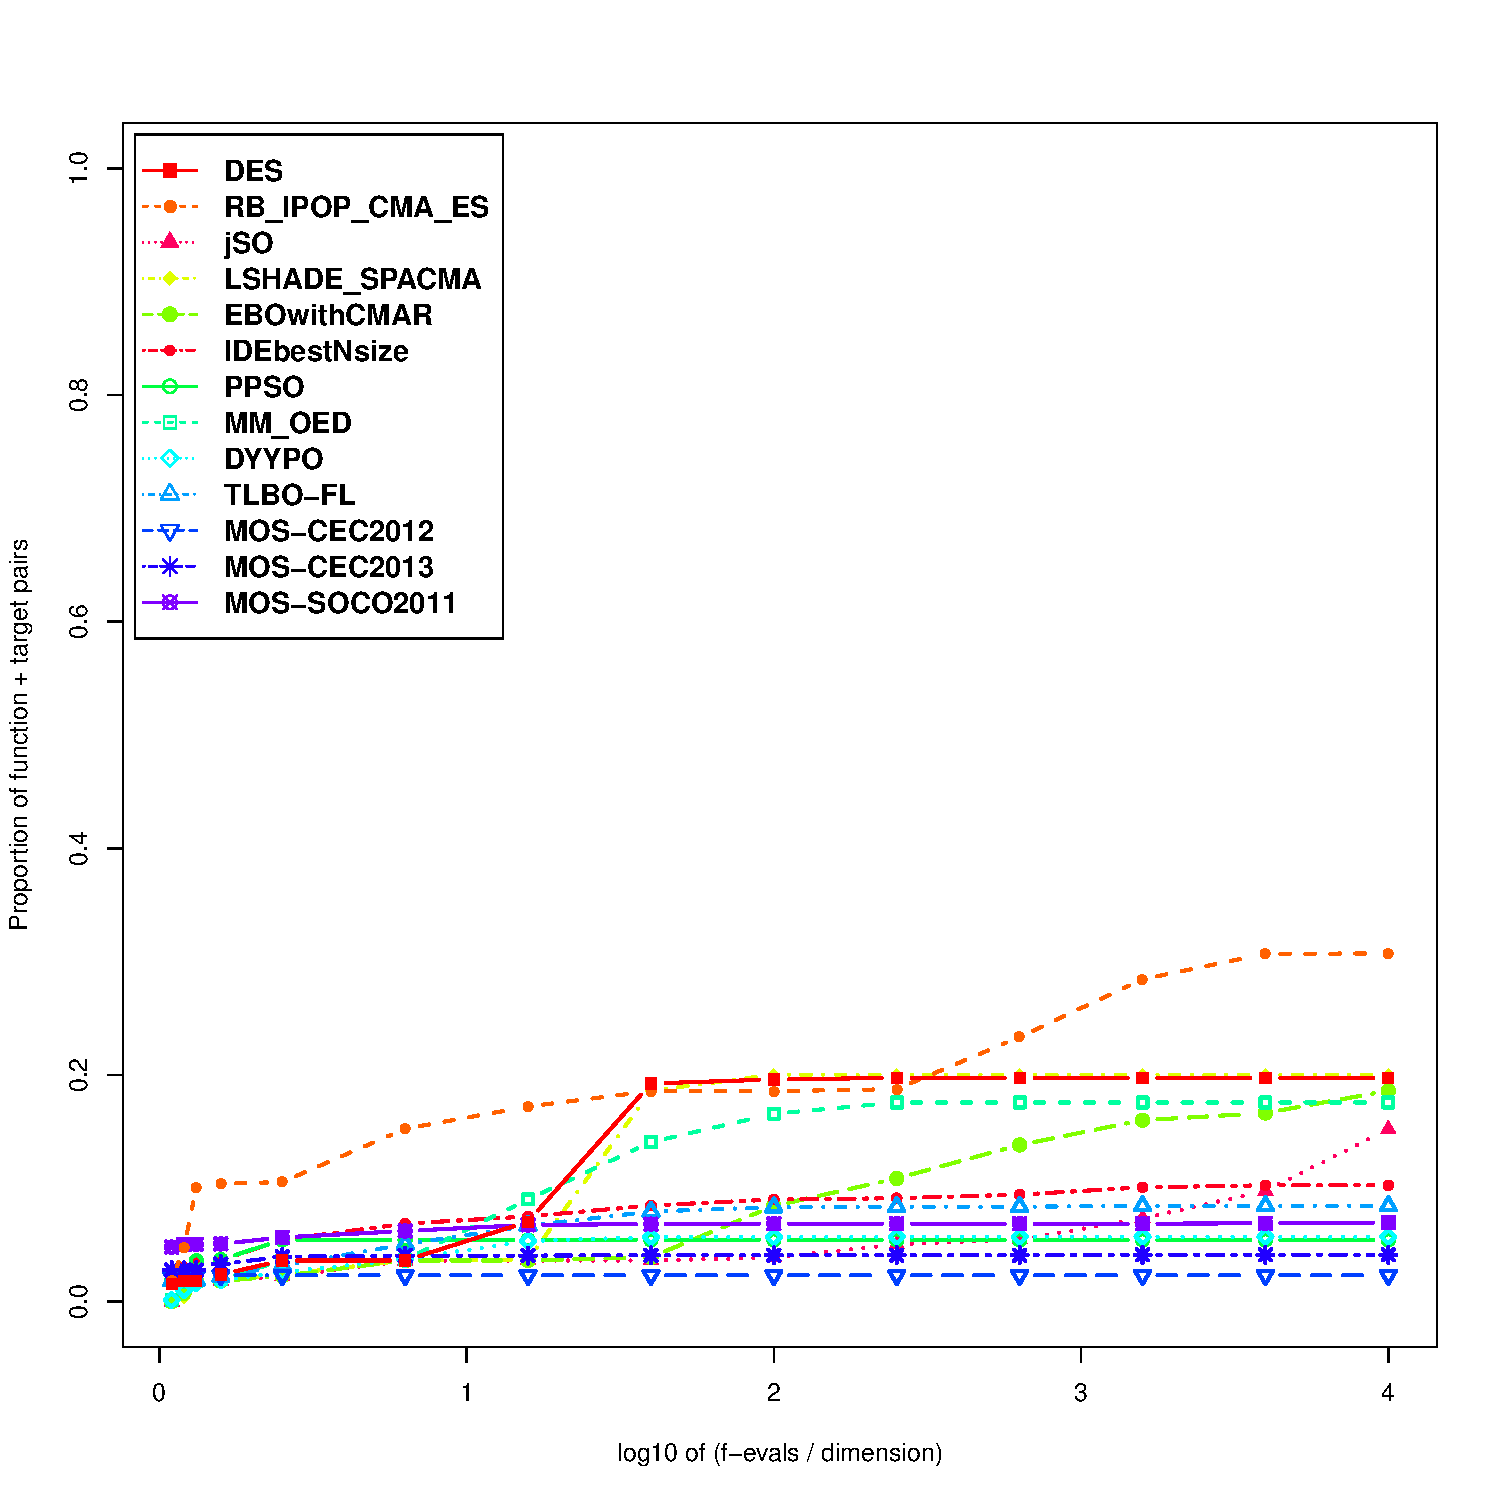
\includegraphics[height=0.9\linewidth,angle=90]{C:/Users/JS/Desktop/Doktorat/EvolutionAlgorithms/IEEEecdf/Plots/singlePlots/Problem=8,N=50.pdf} 
    	\caption{D=50}
    	\end{minipage}%
	}  
  \end{subfigure}%%
  \begin{subfigure}[b]{0.5\linewidth}
    \centering
    \rotatebox[origin=c]{-90}{
        \begin{minipage}{1\linewidth}
        \caption{D=100} 
    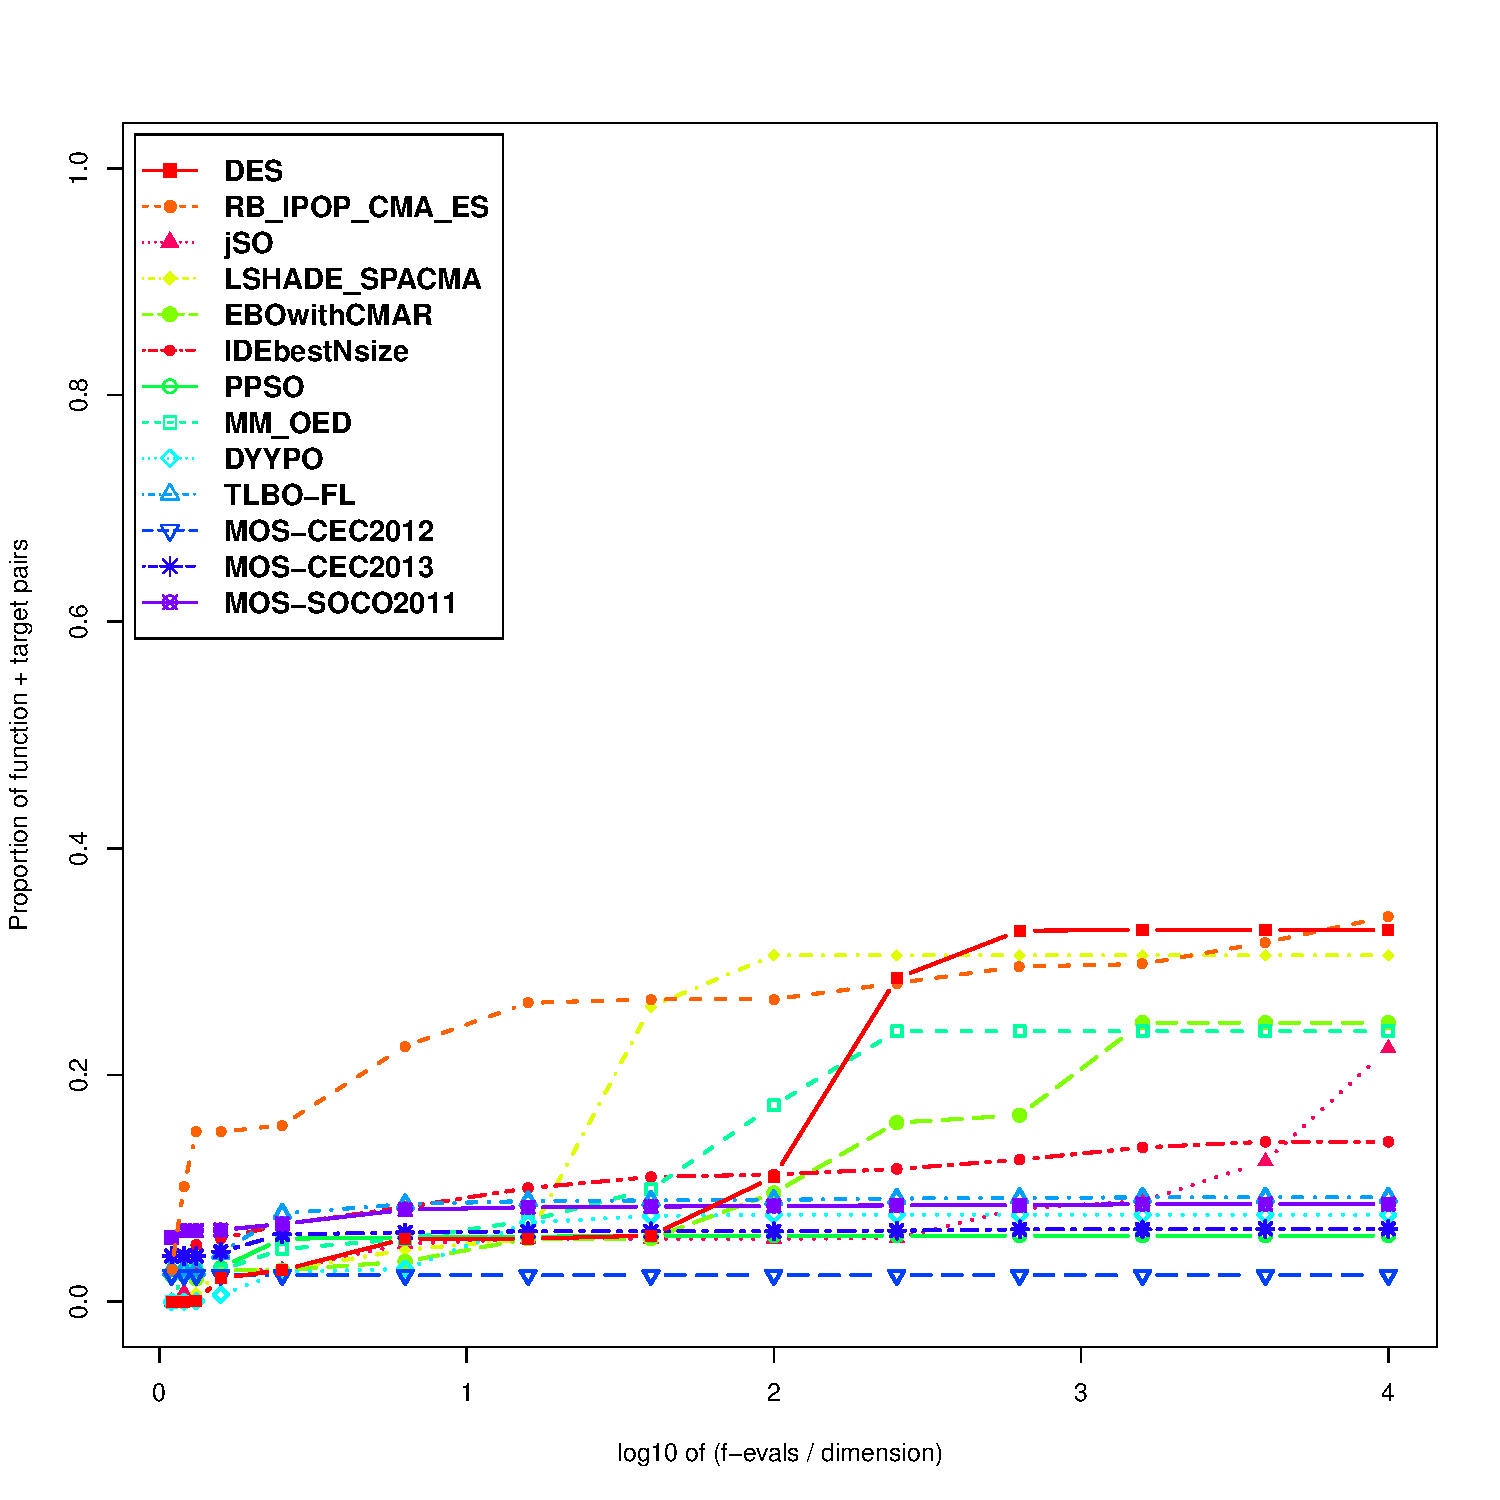
\includegraphics[height=0.9\linewidth,angle=90]{C:/Users/JS/Desktop/Doktorat/EvolutionAlgorithms/IEEEecdf/Plots/singlePlots/Problem=8,N=100.pdf}
    \end{minipage}%
	}   
  \end{subfigure} 
\end{figure}

\end{frame}


\begin{frame}
%\frametitle{CEC2017 Function 9}
\AddToShipoutPictureFG*{
    \AtPageUpperLeft{\put(-135,-12){
    \makebox[\paperwidth][r]{\textcolor{blue}{CEC2017 Function 9}}
    }
    }  
    }%

\begin{figure}[ht] 
    \vspace{-2mm}
\captionsetup[subfigure]{labelformat=empty}
  \begin{subfigure}[b]{0.5\linewidth}
    \centering
      \rotatebox[origin=c]{-90}{
        \begin{minipage}{1\linewidth}
    		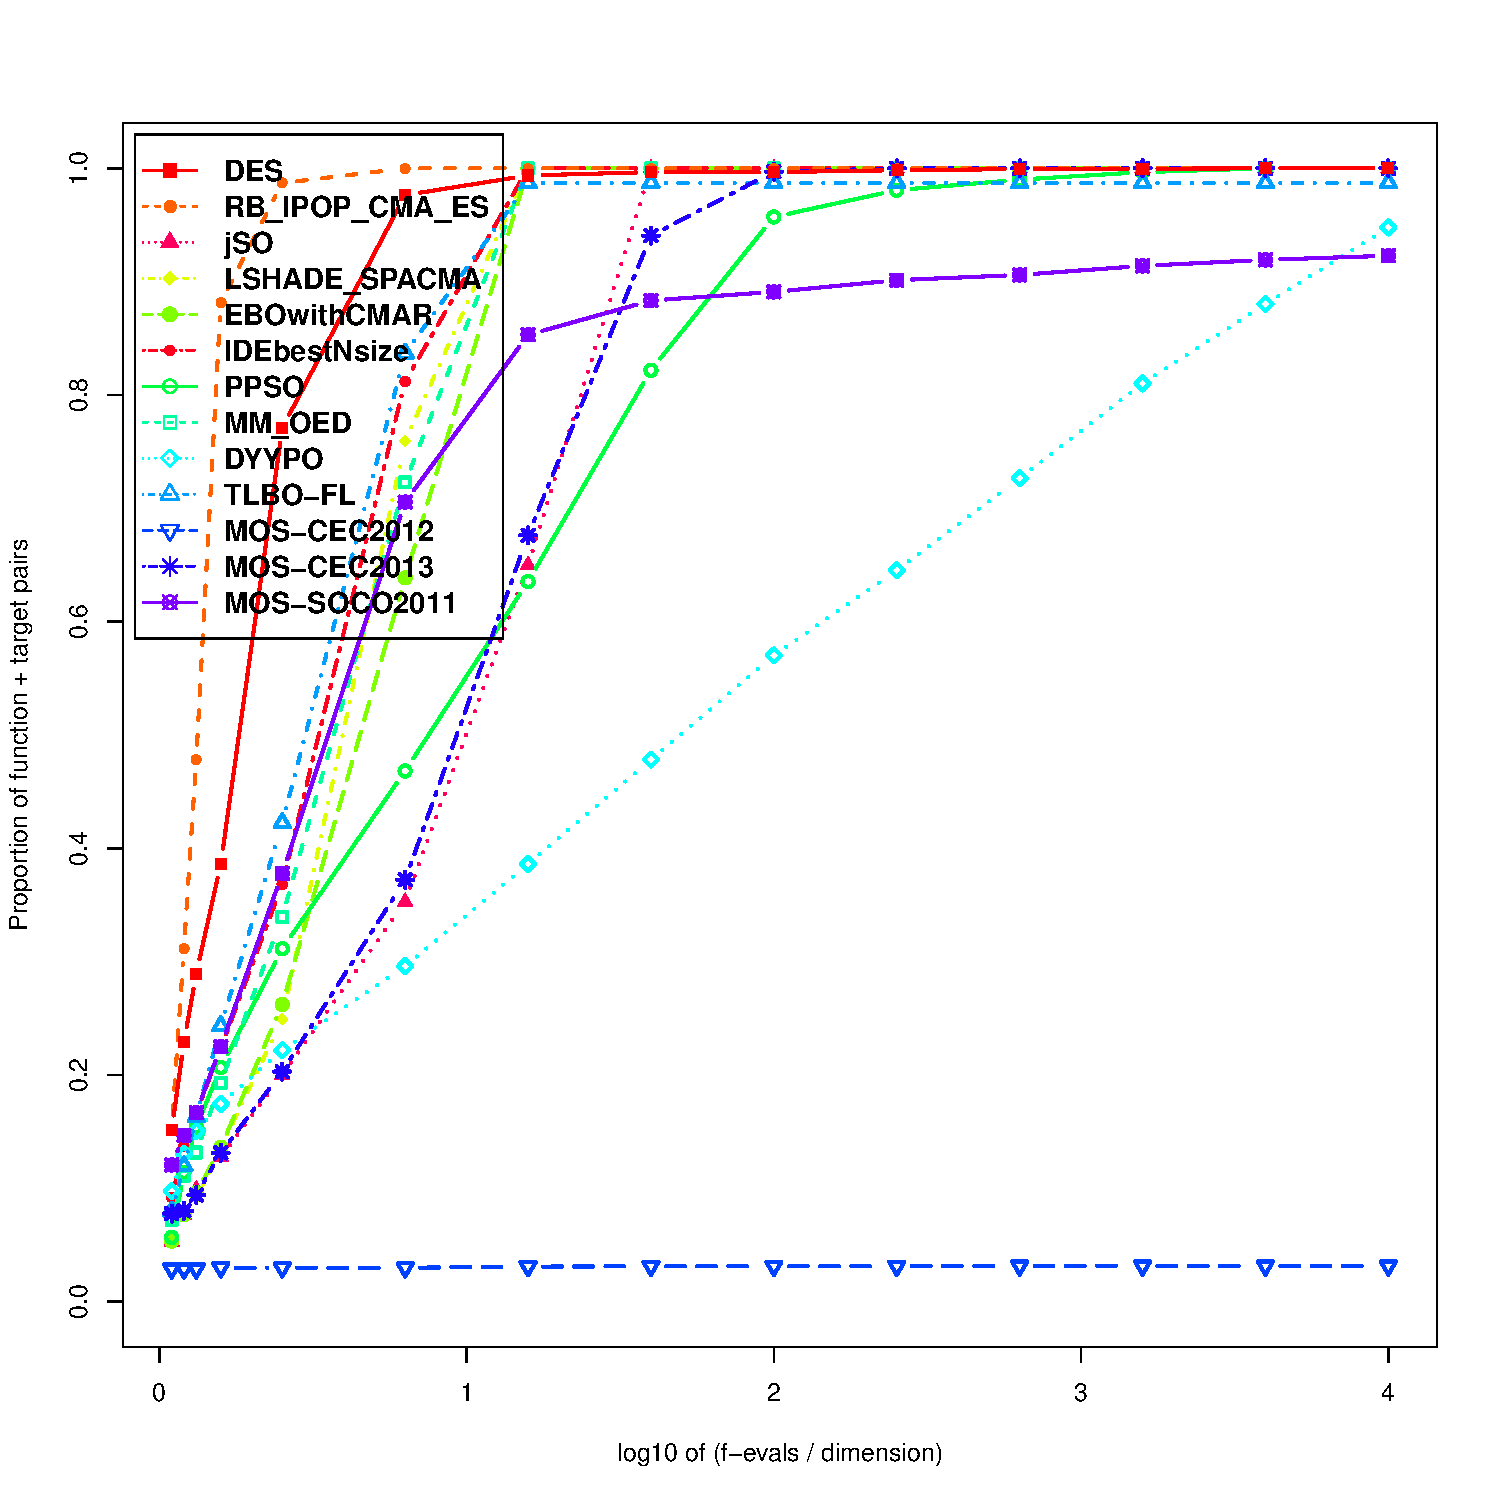
\includegraphics[height=0.9\linewidth,angle=90]{C:/Users/JS/Desktop/Doktorat/EvolutionAlgorithms/IEEEecdf/Plots/singlePlots/Problem=9,N=10.pdf} 
    		\caption{D=10} 
      	\end{minipage}%
	}
    \vspace{-12mm}
  \end{subfigure}%% 
  \begin{subfigure}[b]{0.5\linewidth}
    \centering
    \rotatebox[origin=c]{-90}{
        \begin{minipage}{1\linewidth}
            	\caption{D=30}
    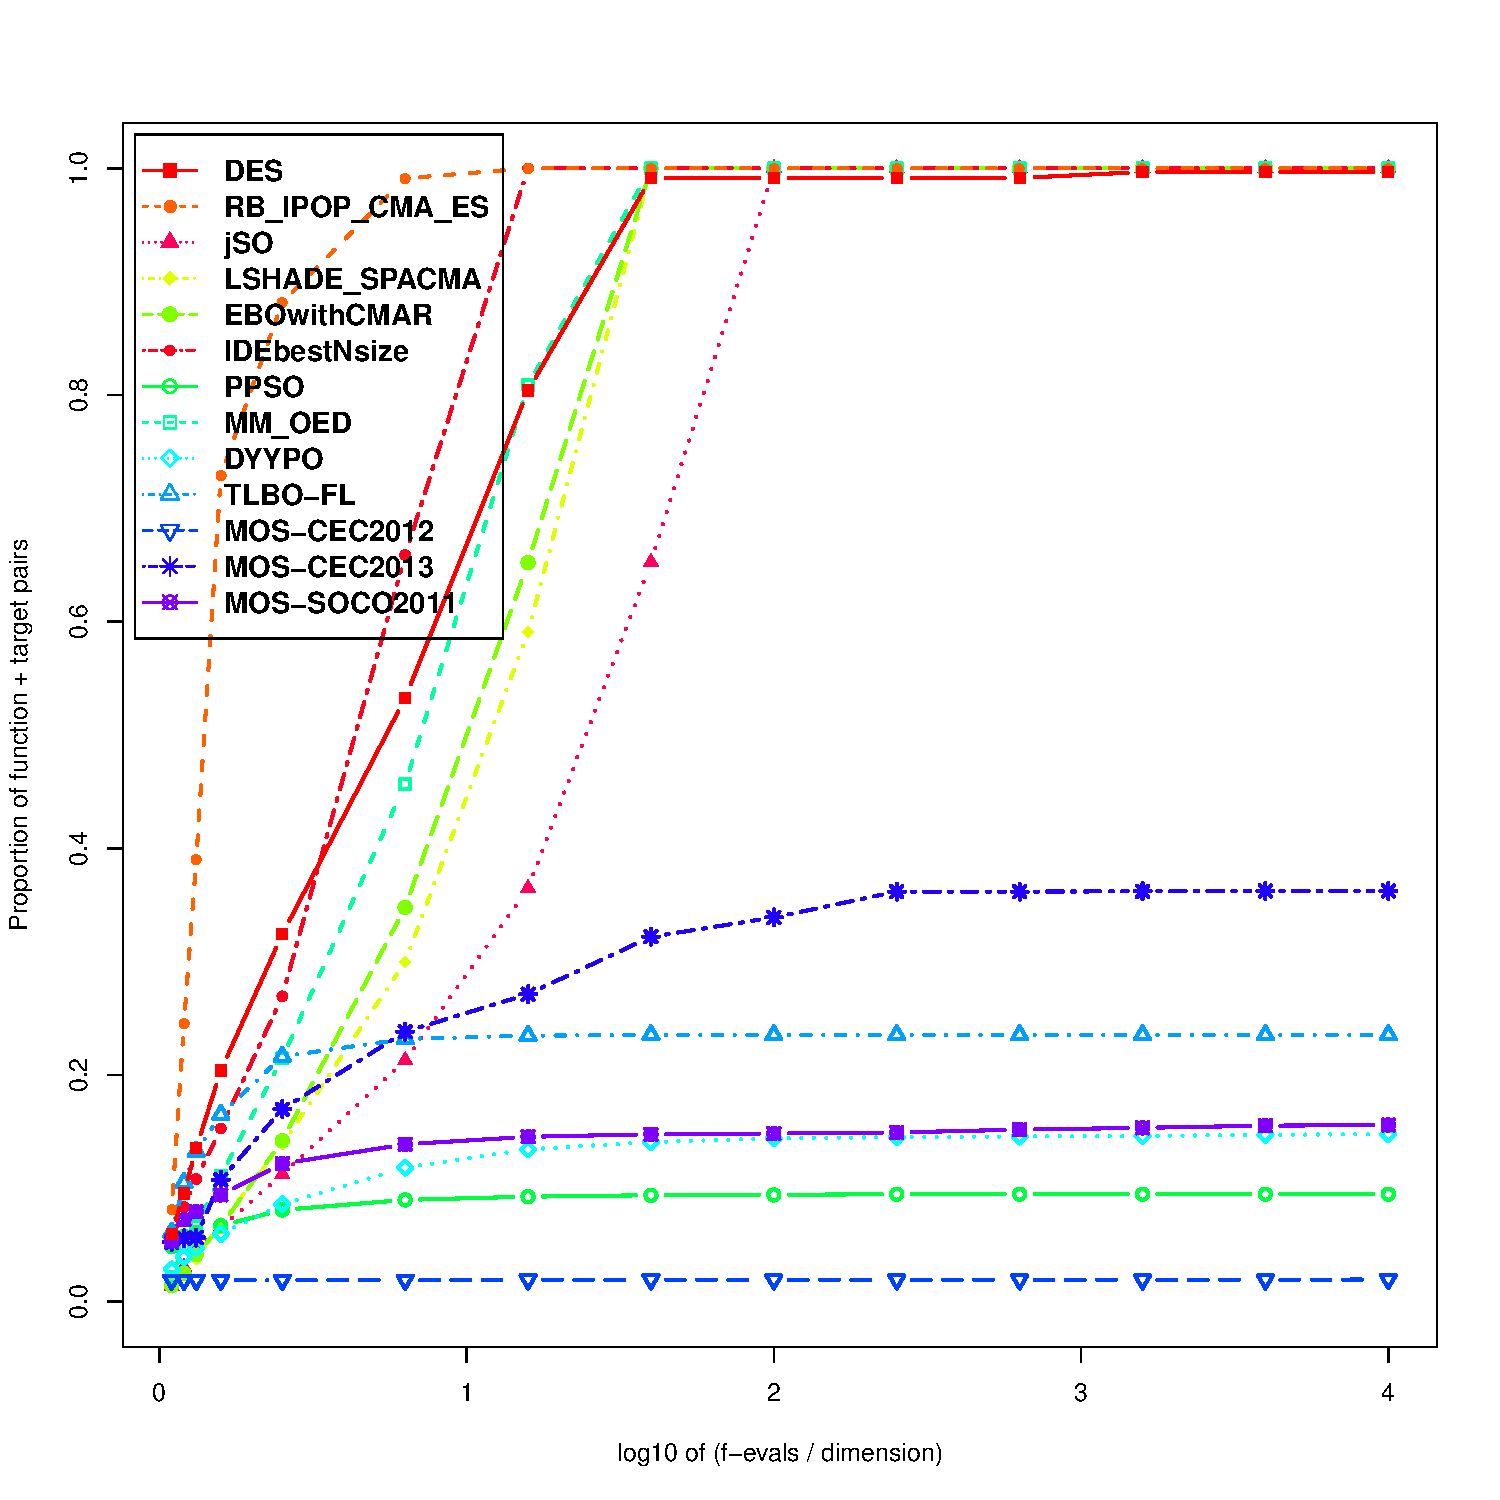
\includegraphics[height=0.9\linewidth,angle=90]{C:/Users/JS/Desktop/Doktorat/EvolutionAlgorithms/IEEEecdf/Plots/singlePlots/Problem=9,N=30.pdf} 
    	\end{minipage}%
	} 
    \vspace{-12mm}
  \end{subfigure} 
  \begin{subfigure}[b]{0.5\linewidth}
    \centering
    \rotatebox[origin=c]{-90}{
        \begin{minipage}{1\linewidth}
    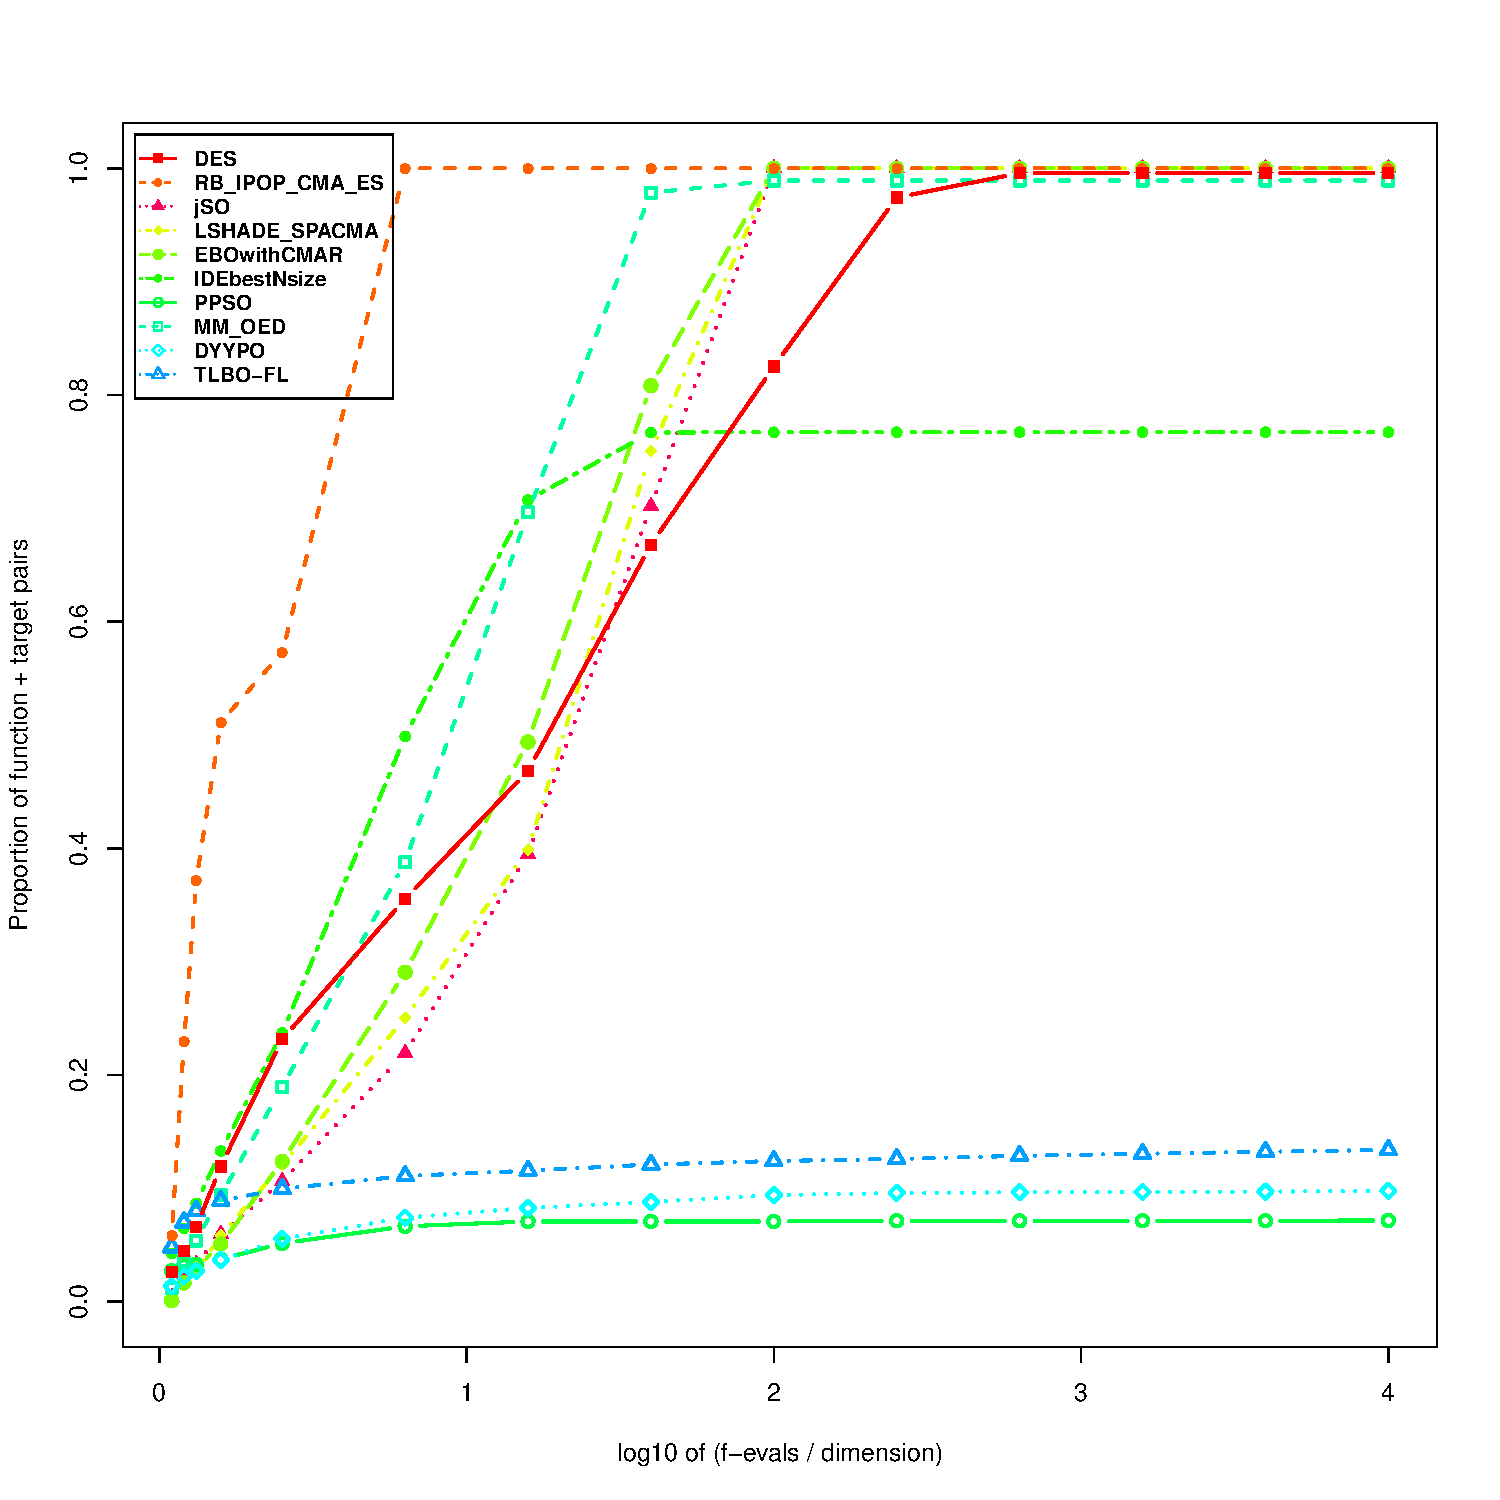
\includegraphics[height=0.9\linewidth,angle=90]{C:/Users/JS/Desktop/Doktorat/EvolutionAlgorithms/IEEEecdf/Plots/singlePlots/Problem=9,N=50.pdf} 
    	\caption{D=50}
    	\end{minipage}%
	}  
  \end{subfigure}%%
  \begin{subfigure}[b]{0.5\linewidth}
    \centering
    \rotatebox[origin=c]{-90}{
        \begin{minipage}{1\linewidth}
        \caption{D=100} 
    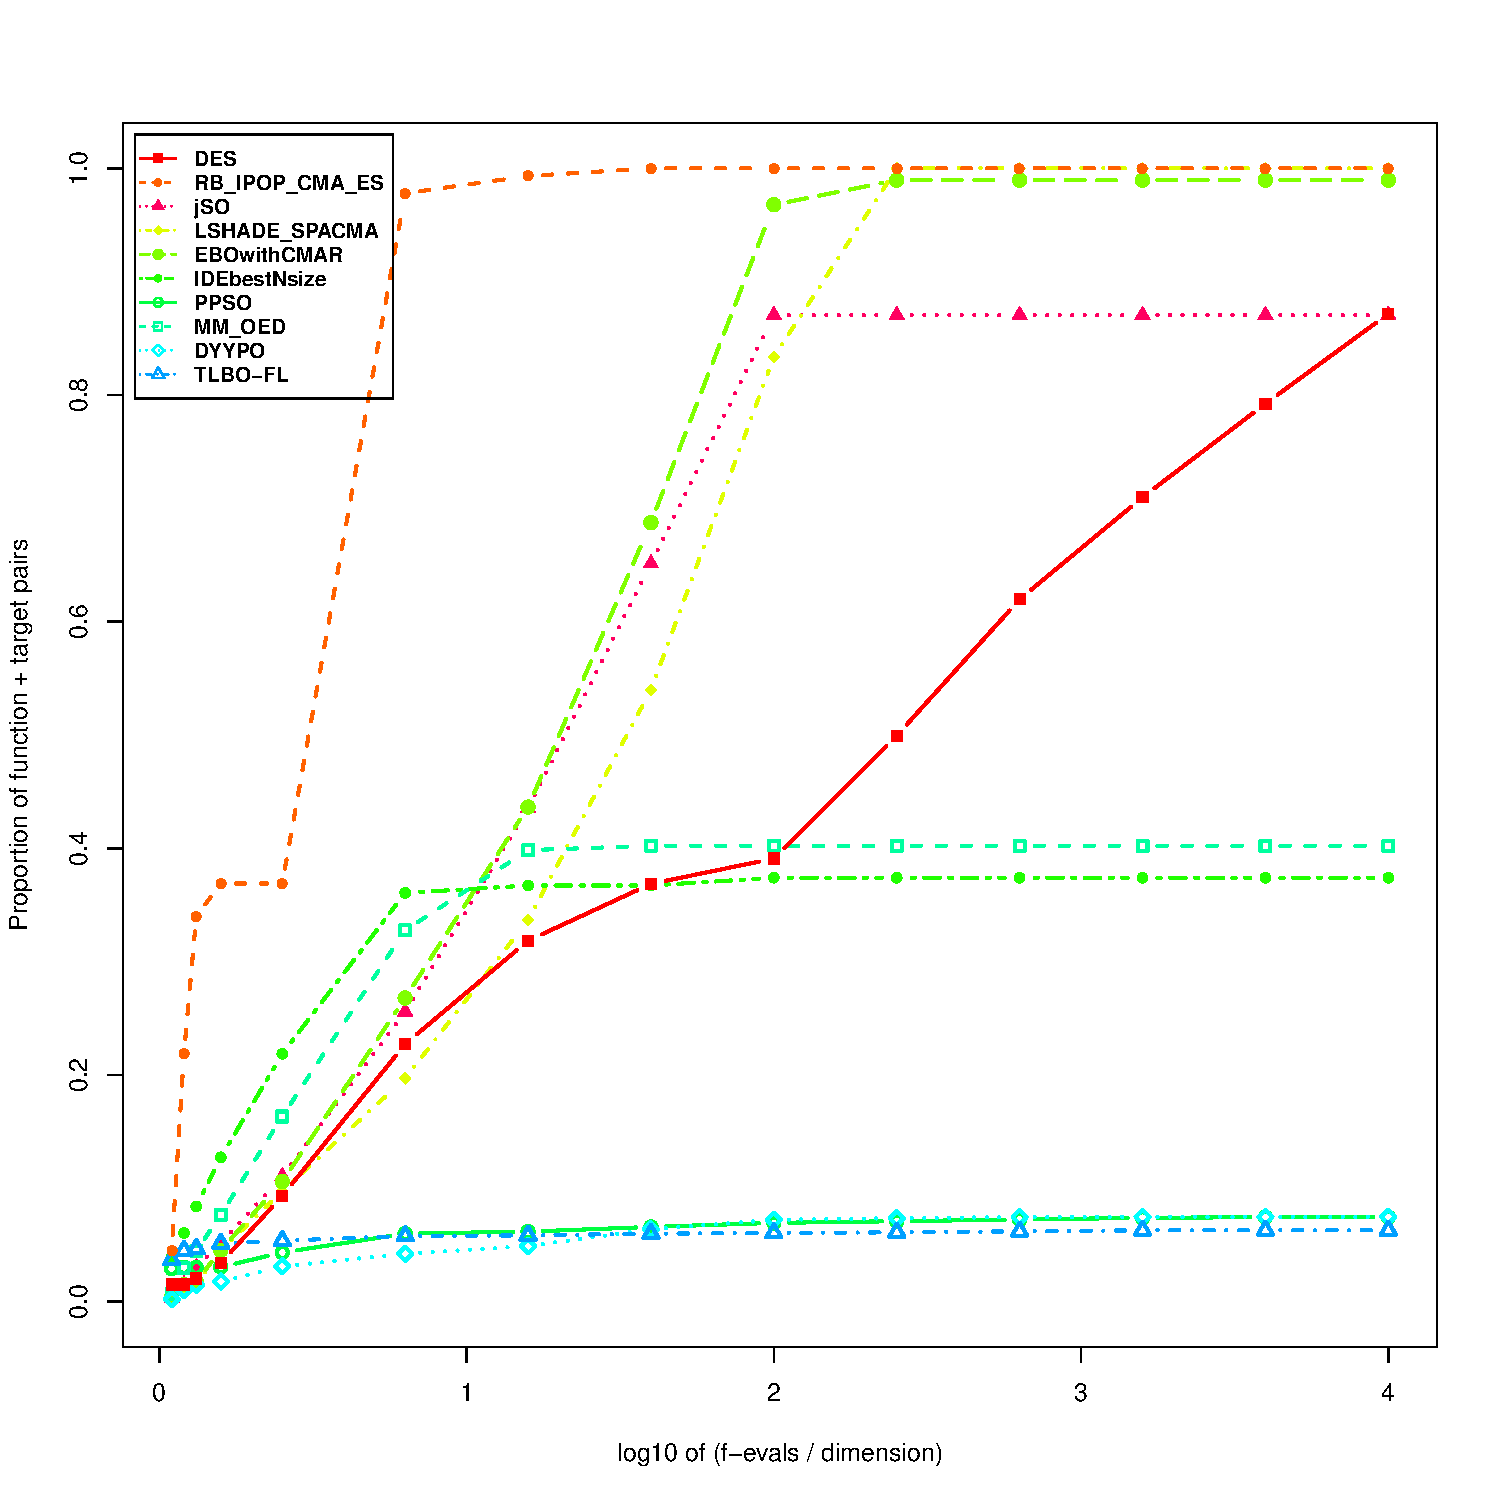
\includegraphics[height=0.9\linewidth,angle=90]{C:/Users/JS/Desktop/Doktorat/EvolutionAlgorithms/IEEEecdf/Plots/singlePlots/Problem=9,N=100.pdf}
    \end{minipage}%
	}   
  \end{subfigure} 
\end{figure}

\end{frame}



\begin{frame}
%\frametitle{CEC2017 Function 10}
\AddToShipoutPictureFG*{
    \AtPageUpperLeft{\put(-135,-12){
    \makebox[\paperwidth][r]{\textcolor{blue}{CEC2017 Function 10}}
    }
    }  
    }%

\begin{figure}[ht] 
    \vspace{-2mm}
\captionsetup[subfigure]{labelformat=empty}
  \begin{subfigure}[b]{0.5\linewidth}
    \centering
      \rotatebox[origin=c]{-90}{
        \begin{minipage}{1\linewidth}
    		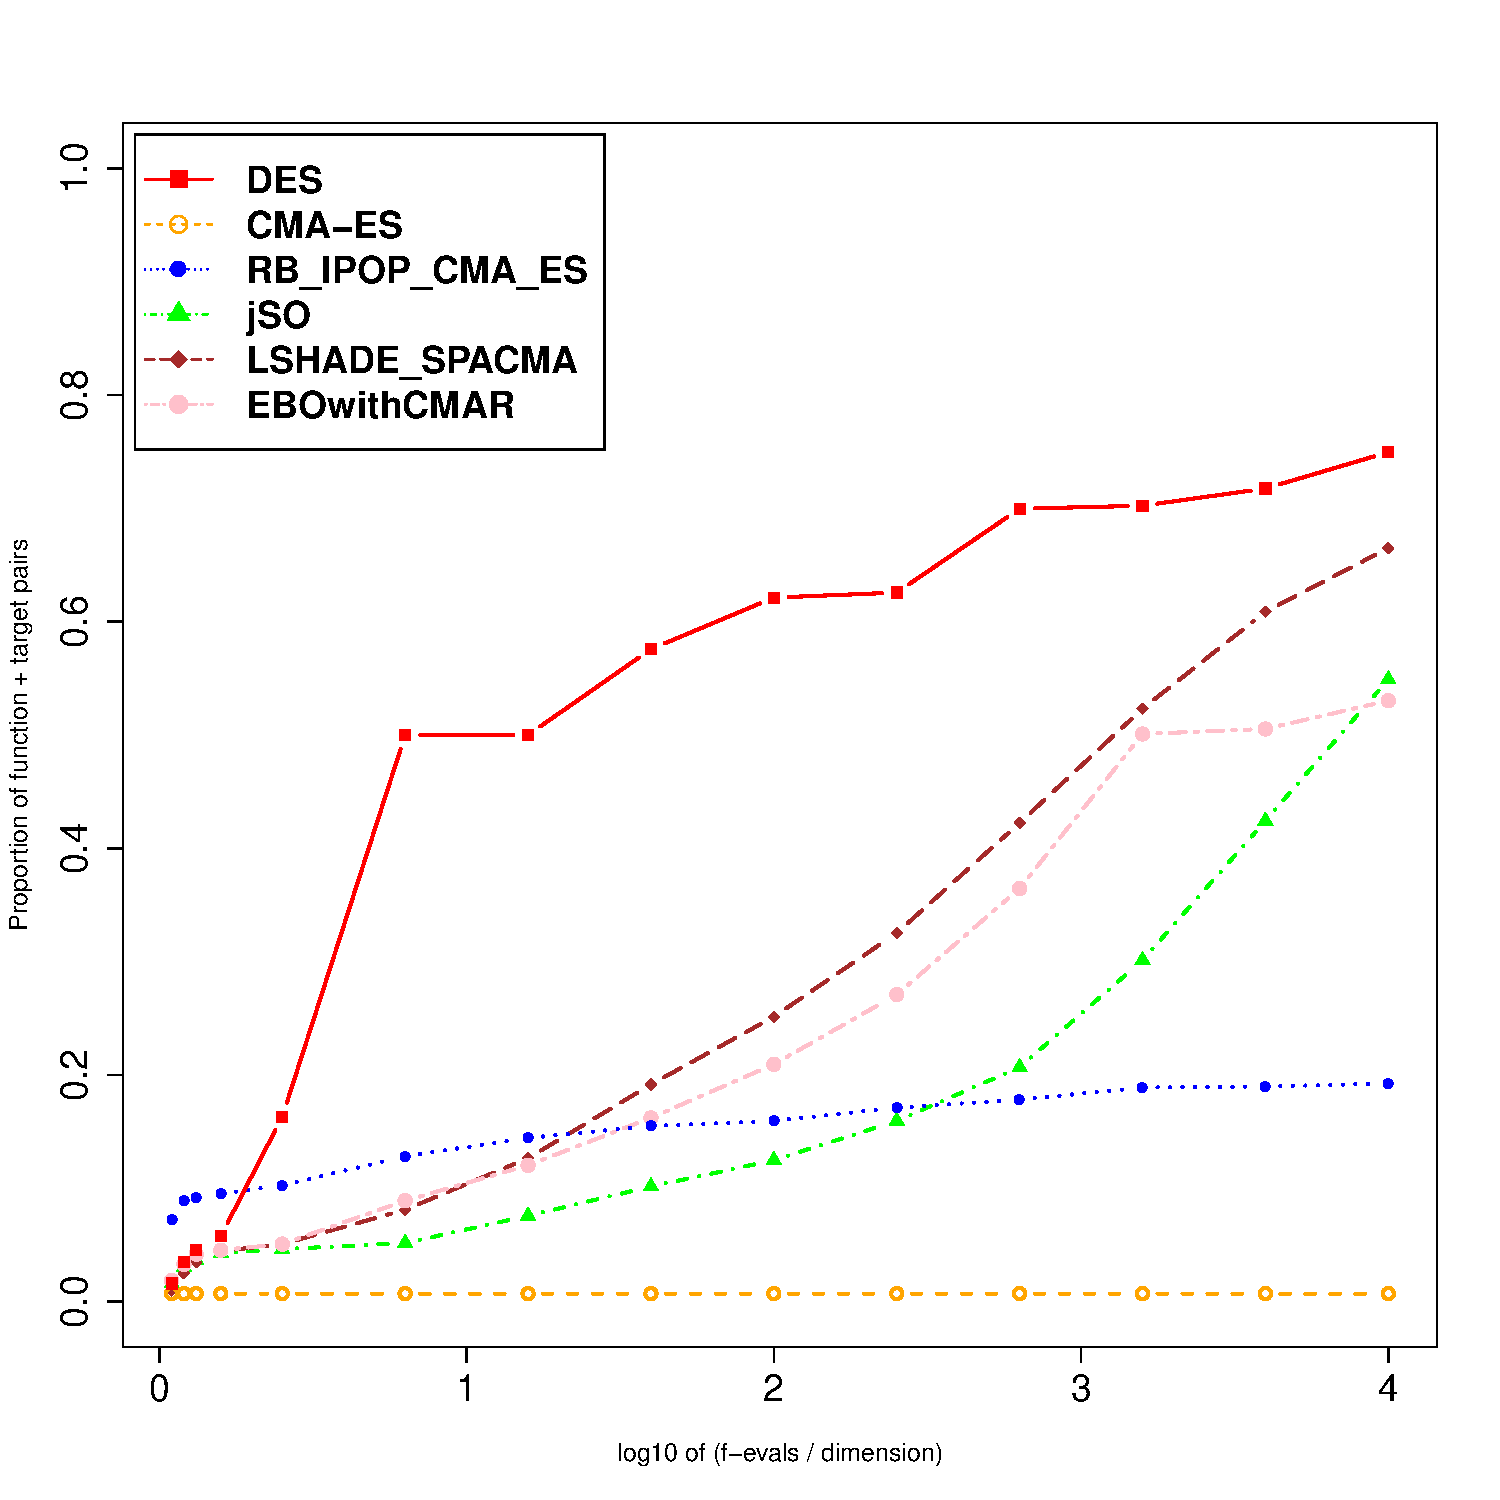
\includegraphics[height=0.9\linewidth,angle=90]{C:/Users/JS/Desktop/Doktorat/EvolutionAlgorithms/IEEEecdf/Plots/singlePlots/Problem=10,N=10.pdf} 
    		\caption{D=10} 
      	\end{minipage}%
	}
    \vspace{-12mm}
  \end{subfigure}%% 
  \begin{subfigure}[b]{0.5\linewidth}
    \centering
    \rotatebox[origin=c]{-90}{
        \begin{minipage}{1\linewidth}
            	\caption{D=30}
    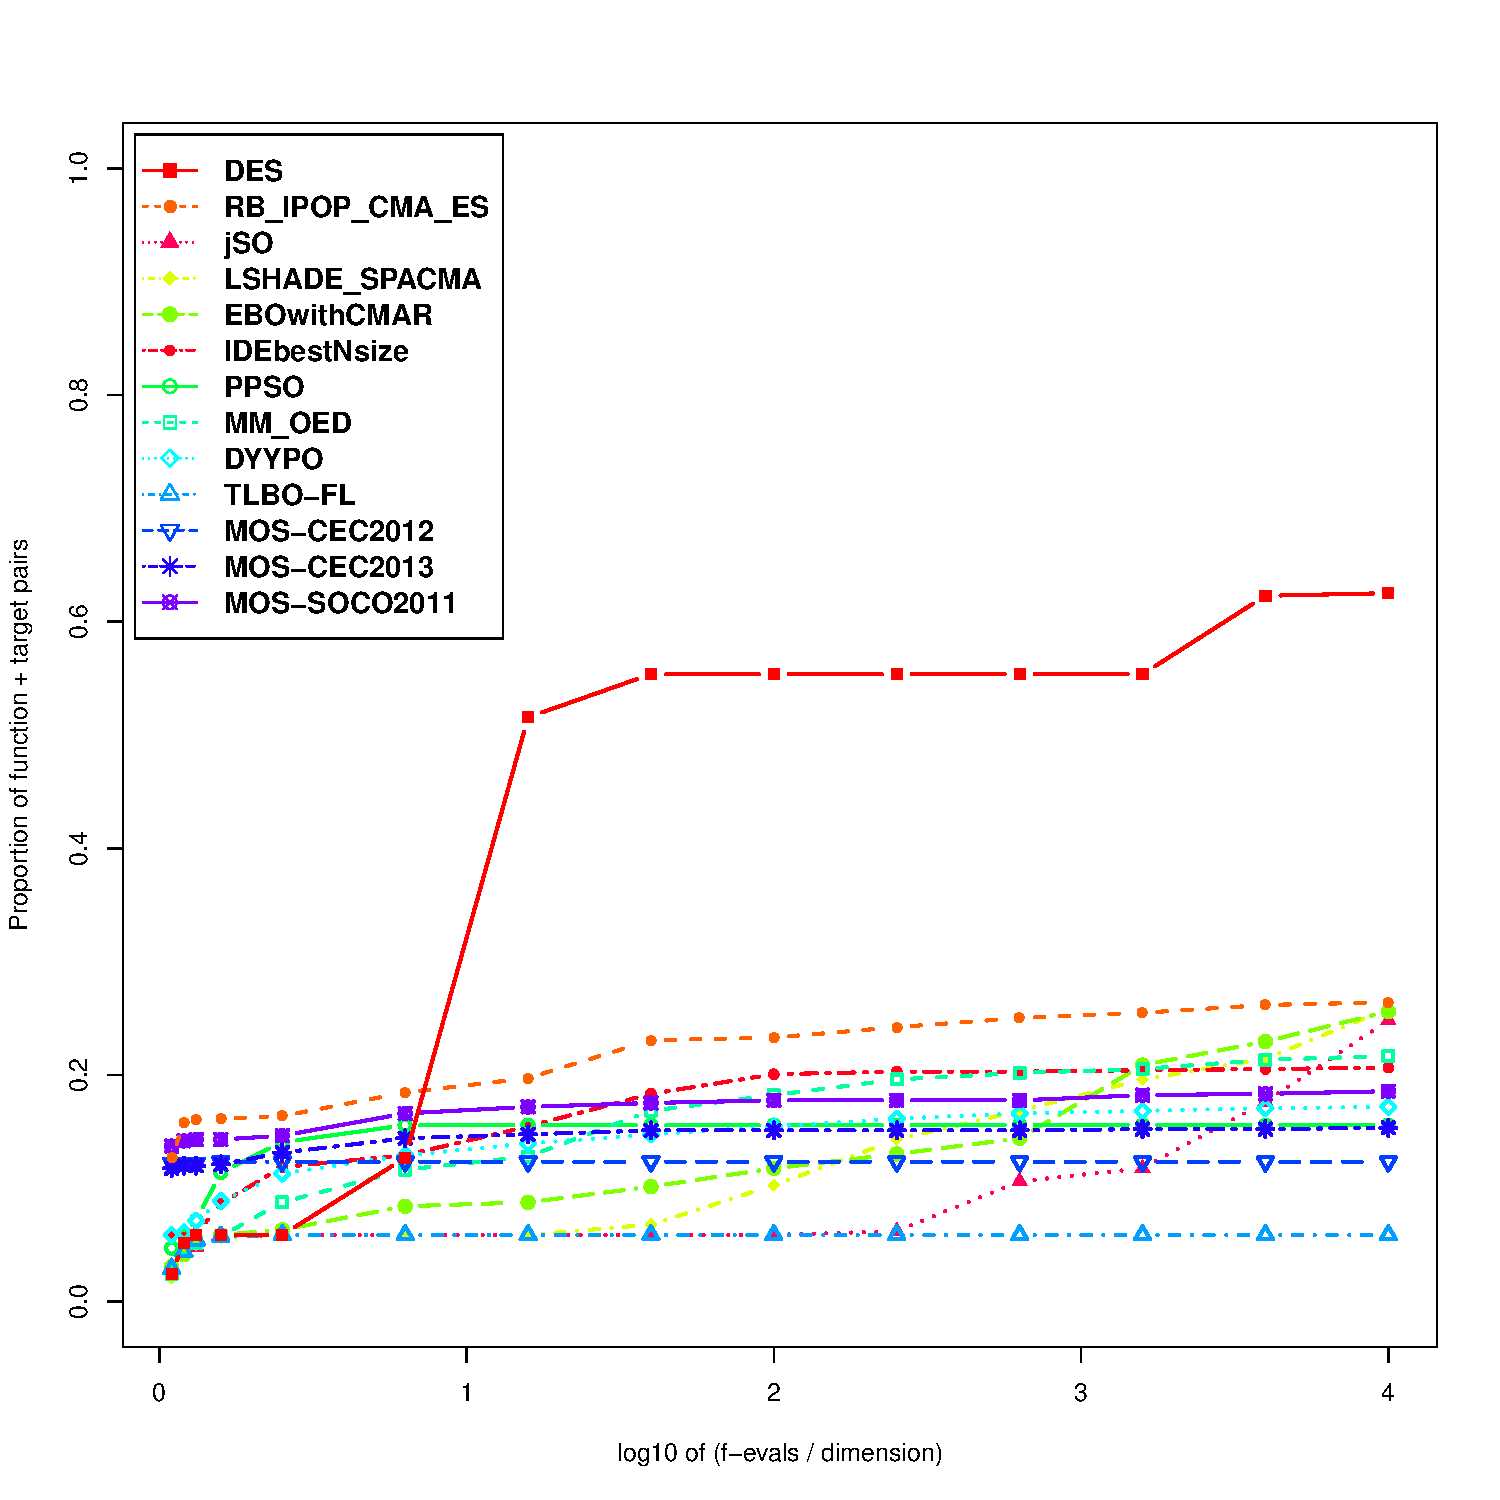
\includegraphics[height=0.9\linewidth,angle=90]{C:/Users/JS/Desktop/Doktorat/EvolutionAlgorithms/IEEEecdf/Plots/singlePlots/Problem=10,N=30.pdf} 
    	\end{minipage}%
	} 
    \vspace{-12mm}
  \end{subfigure} 
  \begin{subfigure}[b]{0.5\linewidth}
    \centering
    \rotatebox[origin=c]{-90}{
        \begin{minipage}{1\linewidth}
    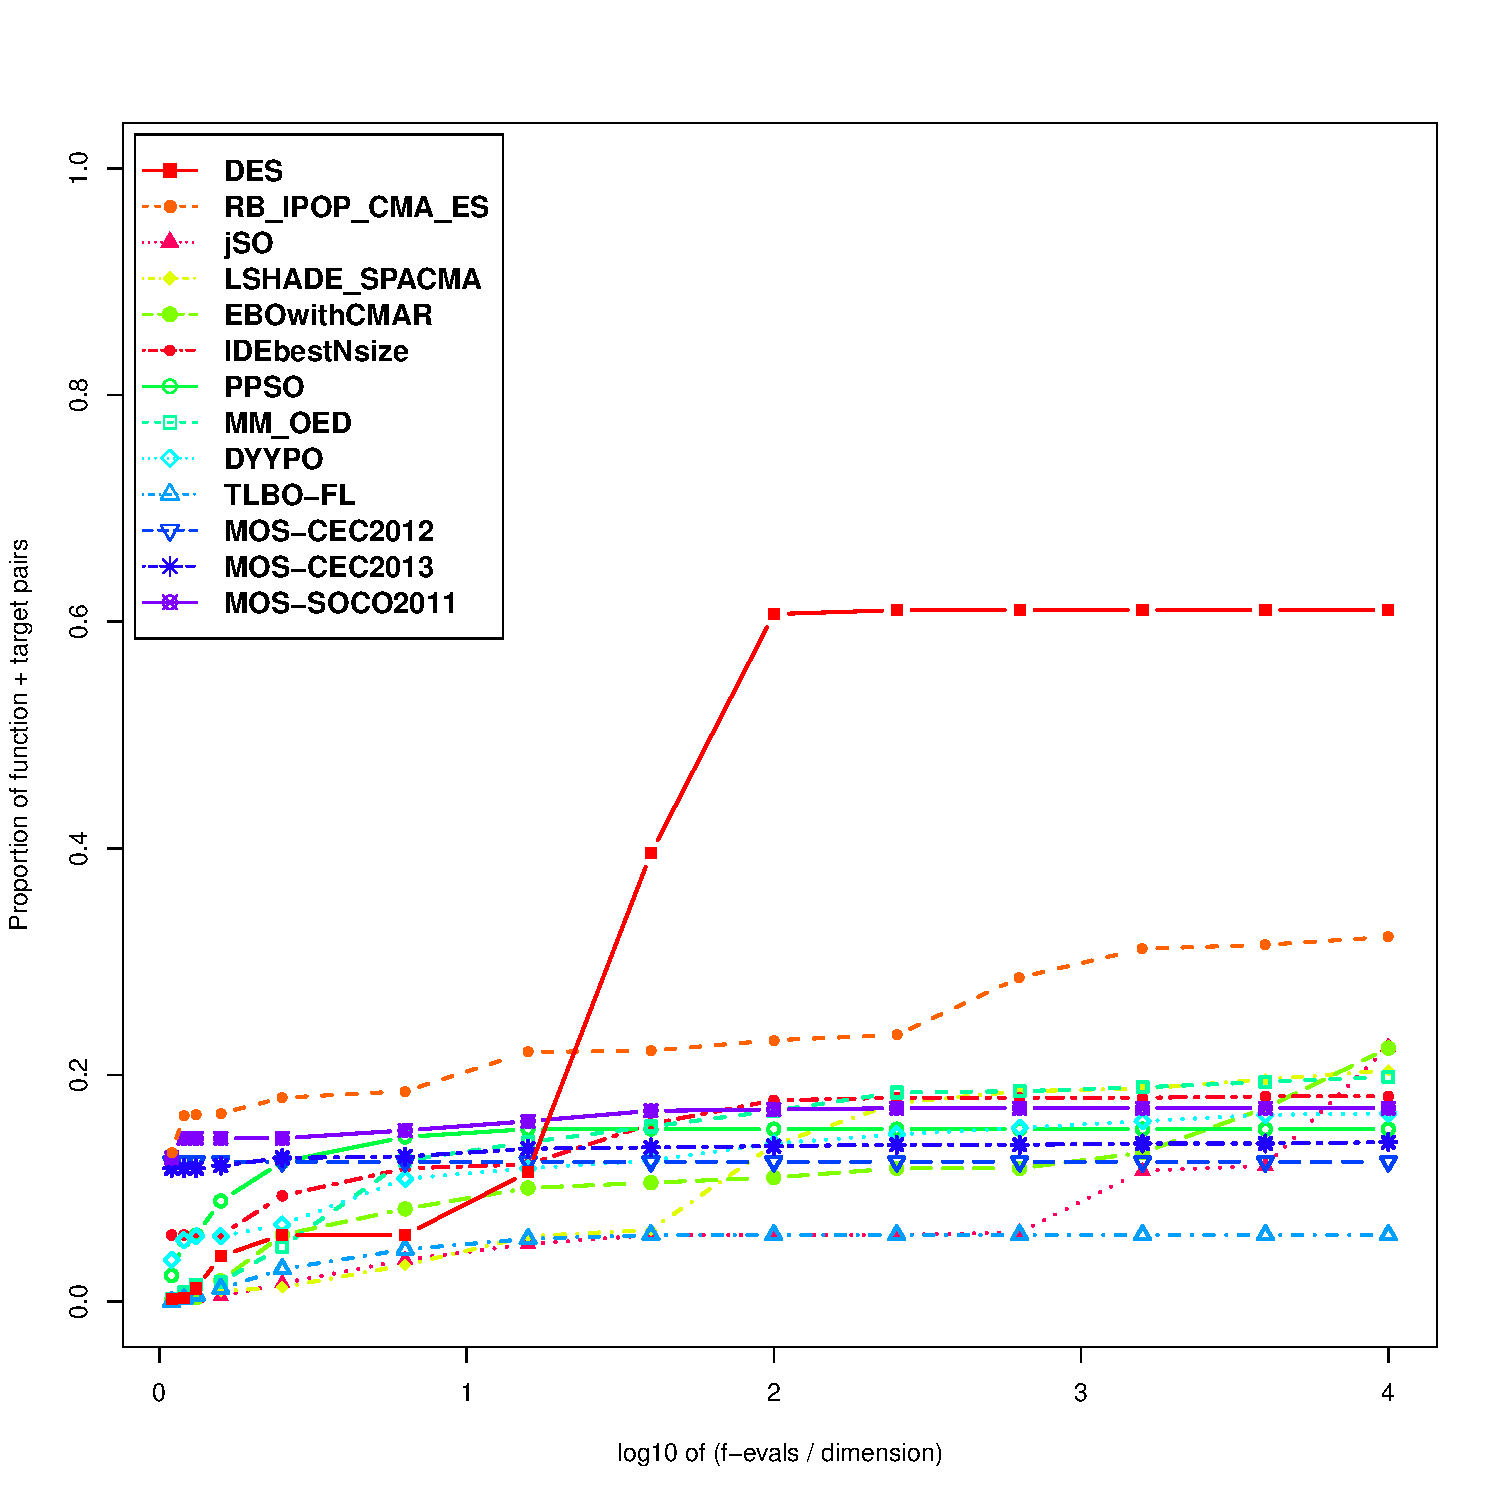
\includegraphics[height=0.9\linewidth,angle=90]{C:/Users/JS/Desktop/Doktorat/EvolutionAlgorithms/IEEEecdf/Plots/singlePlots/Problem=10,N=50.pdf} 
    	\caption{D=50}
    	\end{minipage}%
	}  
  \end{subfigure}%%
  \begin{subfigure}[b]{0.5\linewidth}
    \centering
    \rotatebox[origin=c]{-90}{
        \begin{minipage}{1\linewidth}
        \caption{D=100} 
    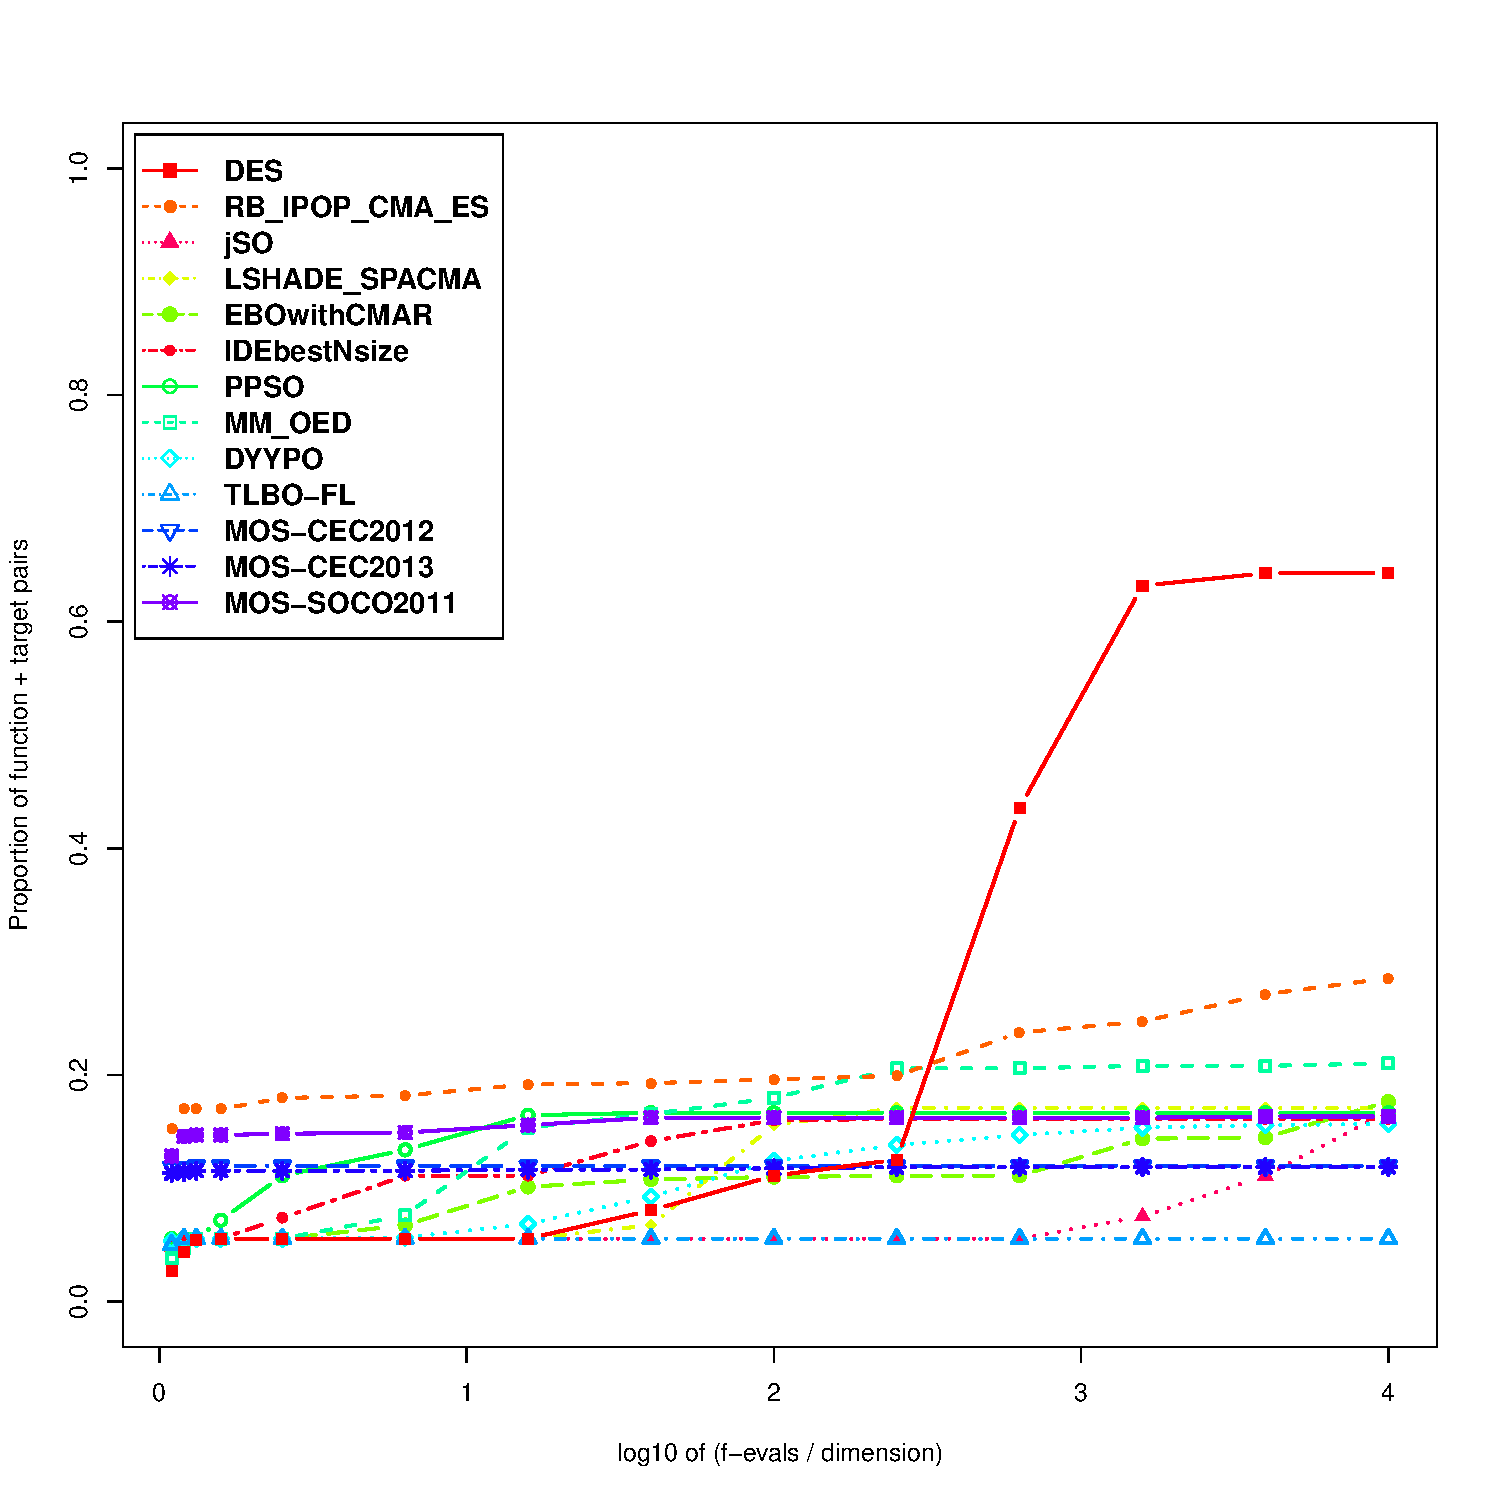
\includegraphics[height=0.9\linewidth,angle=90]{C:/Users/JS/Desktop/Doktorat/EvolutionAlgorithms/IEEEecdf/Plots/singlePlots/Problem=10,N=100.pdf}
    \end{minipage}%
	}   
  \end{subfigure} 
\end{figure}

\end{frame}


\begin{frame}
%\frametitle{CEC2017 Function 11}
\AddToShipoutPictureFG*{
    \AtPageUpperLeft{\put(-135,-12){
    \makebox[\paperwidth][r]{\textcolor{blue}{CEC2017 Function 11}}
    }
    }  
    }%

\begin{figure}[ht] 
    \vspace{-2mm}
\captionsetup[subfigure]{labelformat=empty}
  \begin{subfigure}[b]{0.5\linewidth}
    \centering
      \rotatebox[origin=c]{-90}{
        \begin{minipage}{1\linewidth}
    		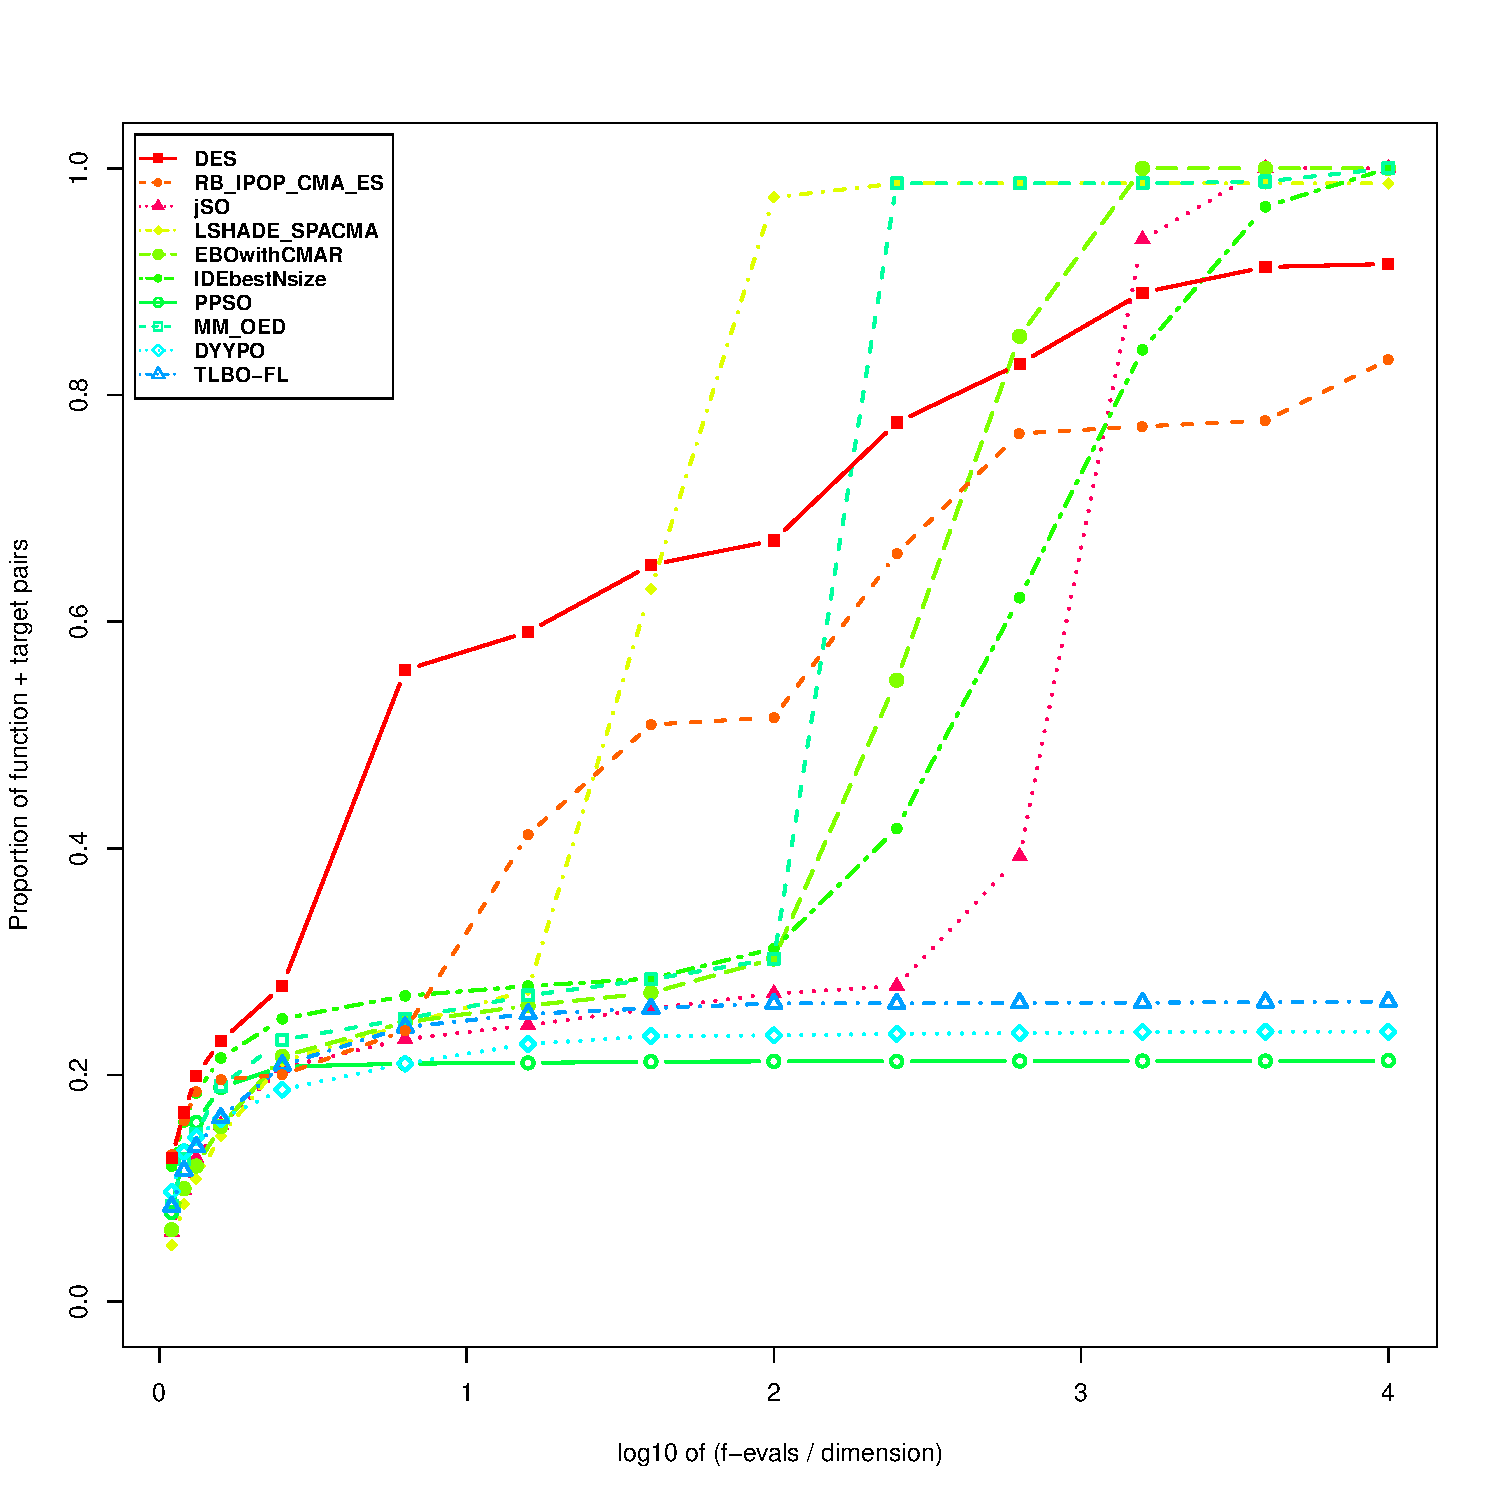
\includegraphics[height=0.9\linewidth,angle=90]{C:/Users/JS/Desktop/Doktorat/EvolutionAlgorithms/IEEEecdf/Plots/singlePlots/Problem=11,N=10.pdf} 
    		\caption{D=10} 
      	\end{minipage}%
	}
    \vspace{-12mm}
  \end{subfigure}%% 
  \begin{subfigure}[b]{0.5\linewidth}
    \centering
    \rotatebox[origin=c]{-90}{
        \begin{minipage}{1\linewidth}
            	\caption{D=30}
    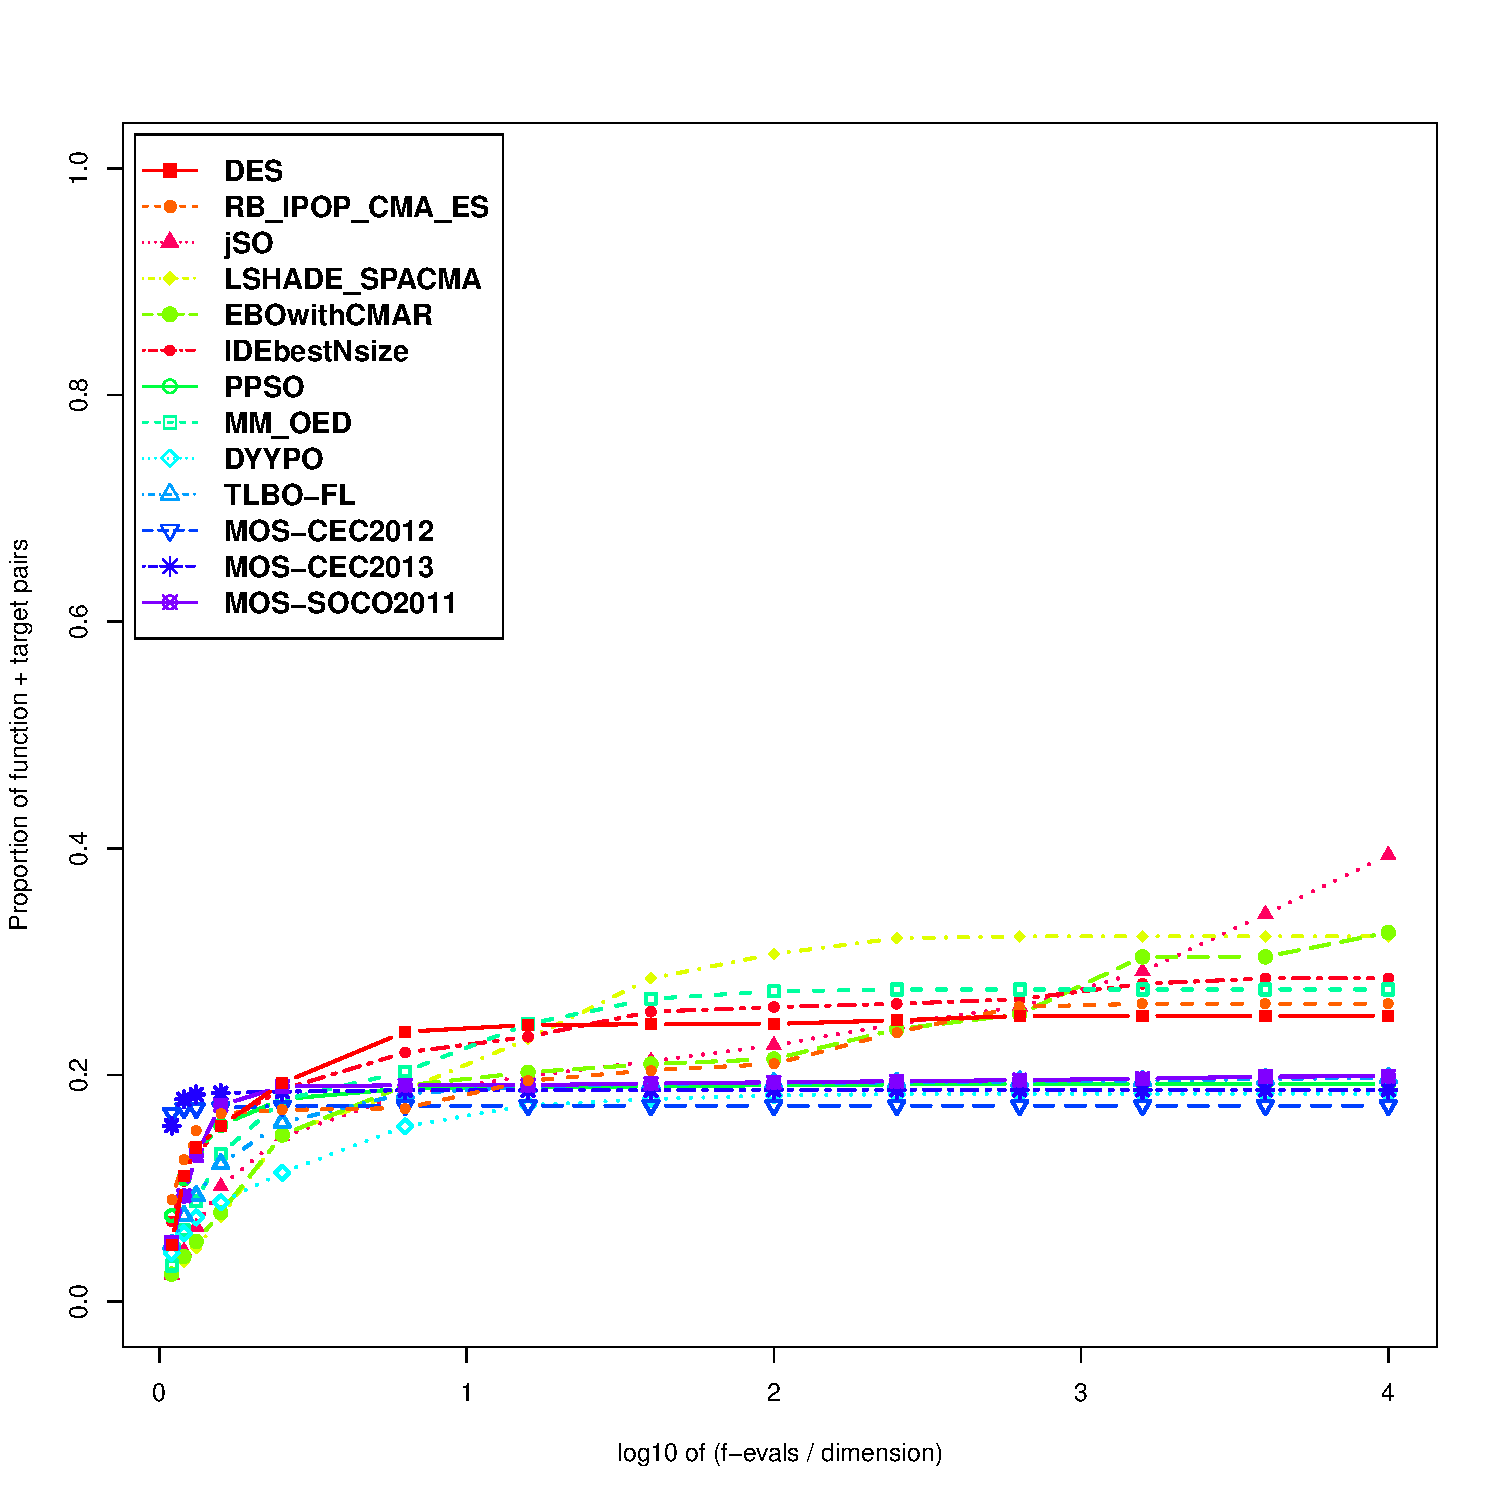
\includegraphics[height=0.9\linewidth,angle=90]{C:/Users/JS/Desktop/Doktorat/EvolutionAlgorithms/IEEEecdf/Plots/singlePlots/Problem=11,N=30.pdf} 
    	\end{minipage}%
	} 
    \vspace{-12mm}
  \end{subfigure} 
  \begin{subfigure}[b]{0.5\linewidth}
    \centering
    \rotatebox[origin=c]{-90}{
        \begin{minipage}{1\linewidth}
    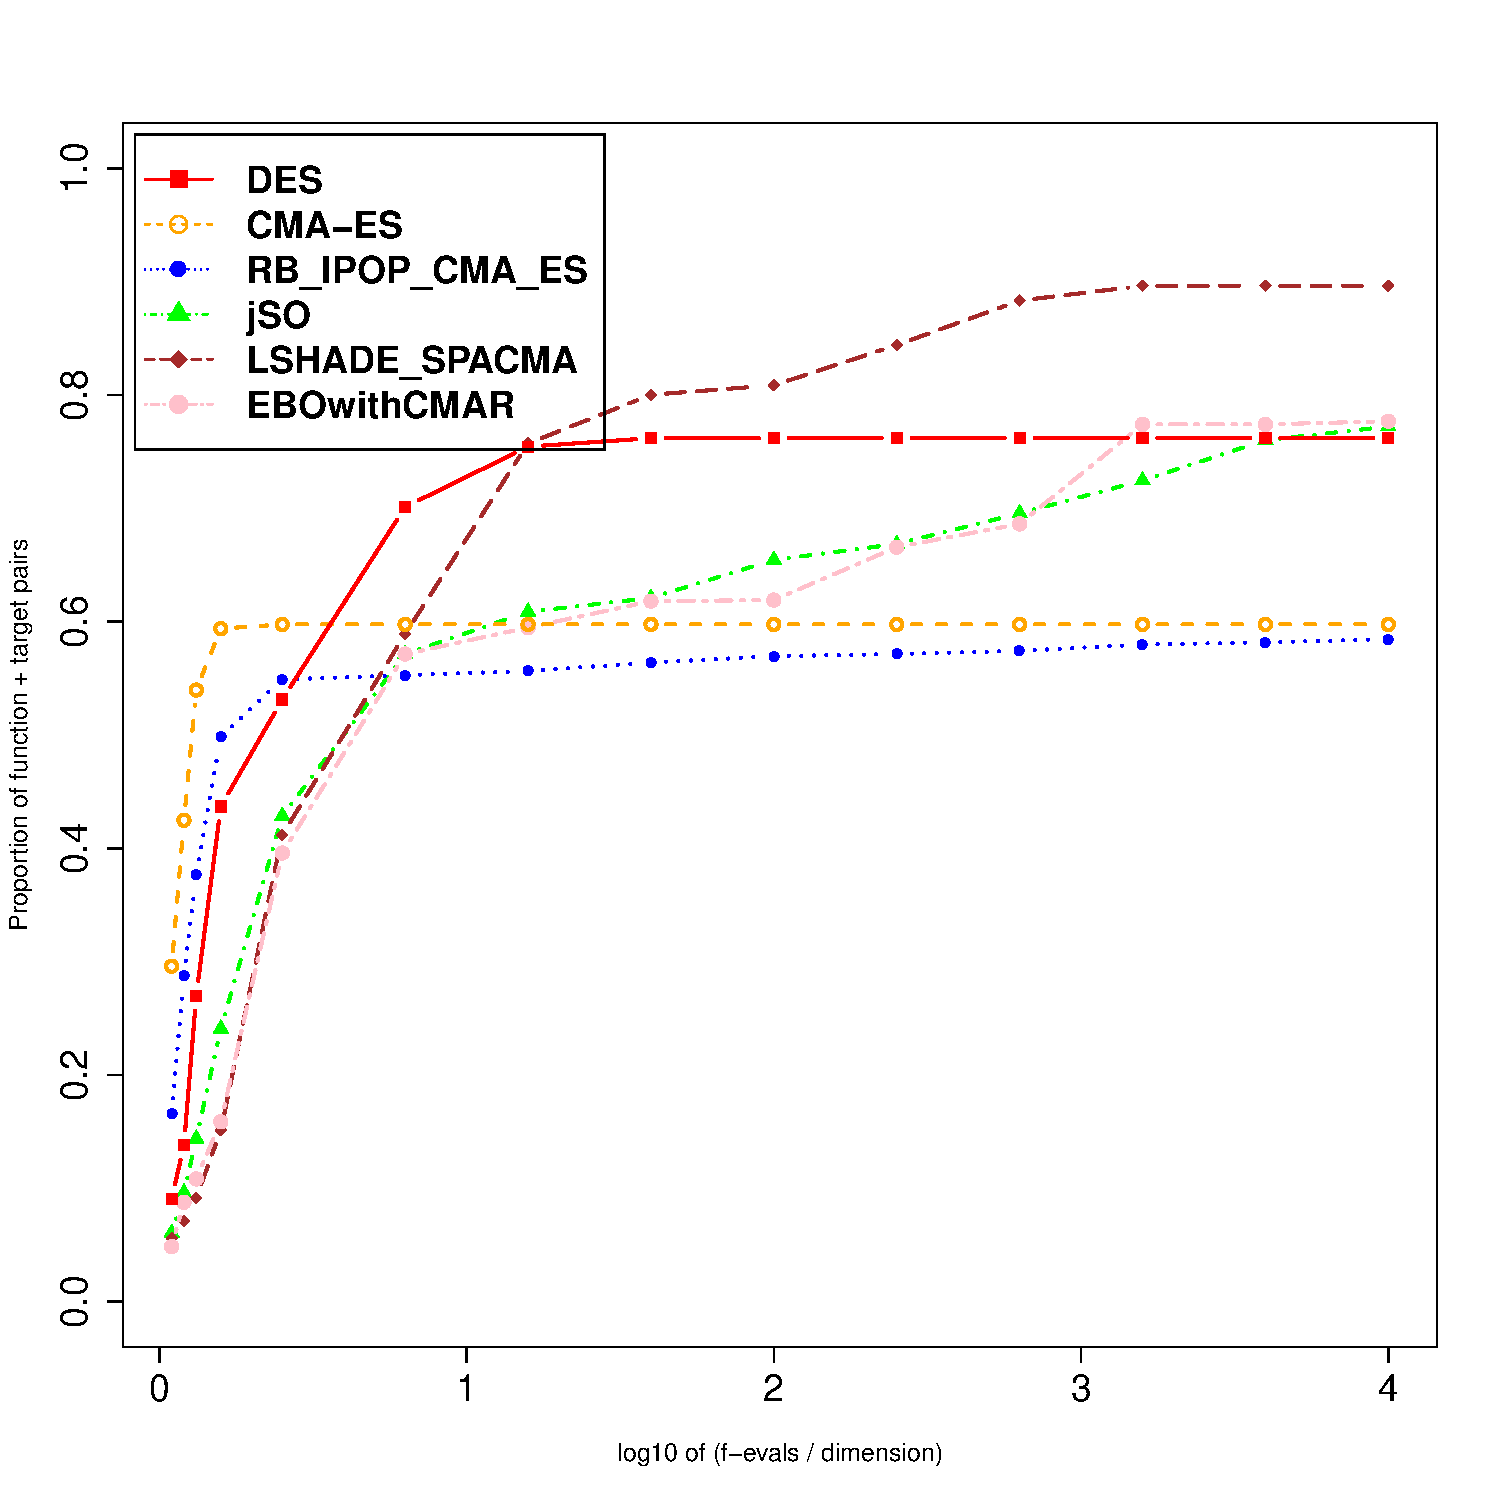
\includegraphics[height=0.9\linewidth,angle=90]{C:/Users/JS/Desktop/Doktorat/EvolutionAlgorithms/IEEEecdf/Plots/singlePlots/Problem=11,N=50.pdf} 
    	\caption{D=50}
    	\end{minipage}%
	}  
  \end{subfigure}%%
  \begin{subfigure}[b]{0.5\linewidth}
    \centering
    \rotatebox[origin=c]{-90}{
        \begin{minipage}{1\linewidth}
        \caption{D=100} 
    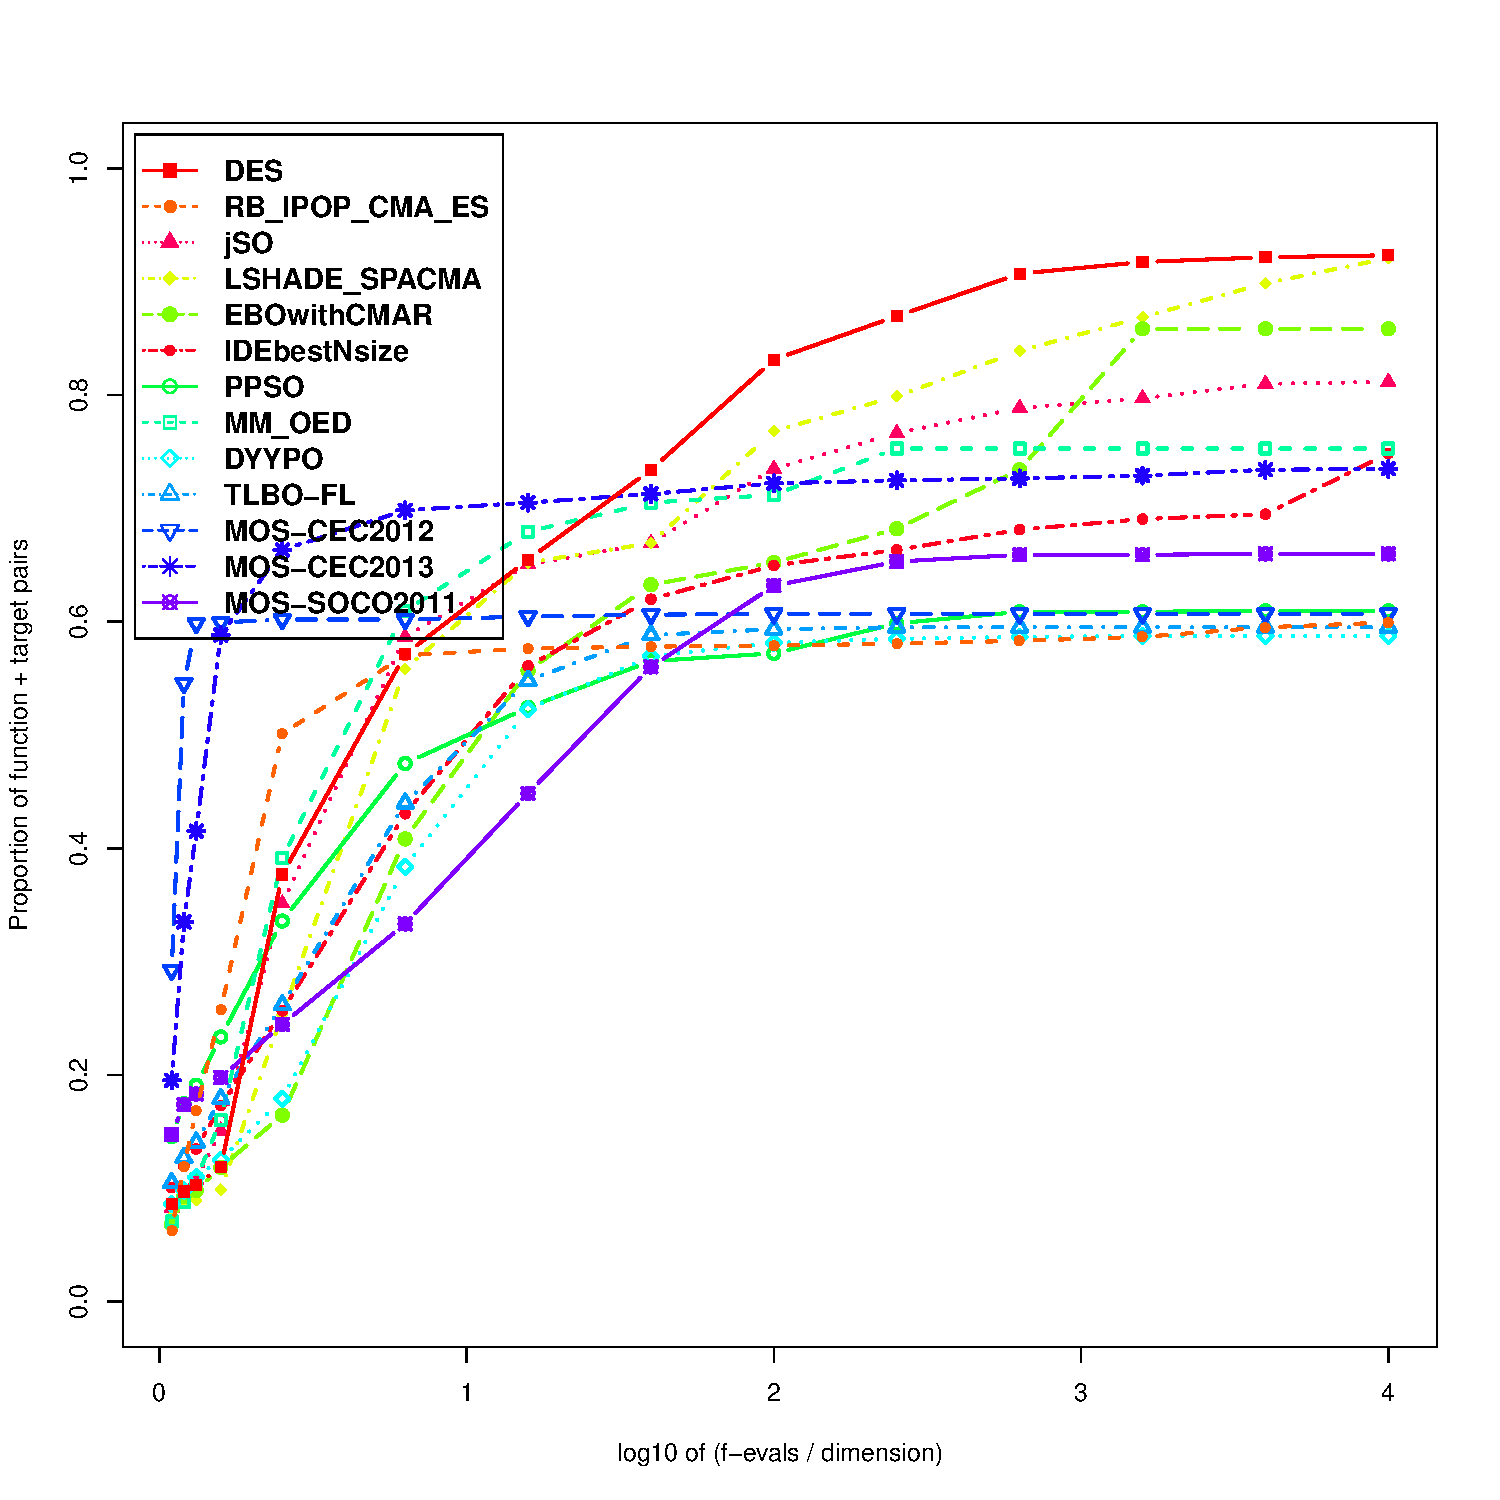
\includegraphics[height=0.9\linewidth,angle=90]{C:/Users/JS/Desktop/Doktorat/EvolutionAlgorithms/IEEEecdf/Plots/singlePlots/Problem=11,N=100.pdf}
    \end{minipage}%
	}   
  \end{subfigure} 
\end{figure}

\end{frame}

\begin{frame}
%\frametitle{CEC2017 Function 12}
\AddToShipoutPictureFG*{
    \AtPageUpperLeft{\put(-135,-12){
    \makebox[\paperwidth][r]{\textcolor{blue}{CEC2017 Function 12}}
    }
    }  
    }%

\begin{figure}[ht] 
    \vspace{-2mm}
\captionsetup[subfigure]{labelformat=empty}
  \begin{subfigure}[b]{0.5\linewidth}
    \centering
      \rotatebox[origin=c]{-90}{
        \begin{minipage}{1\linewidth}
    		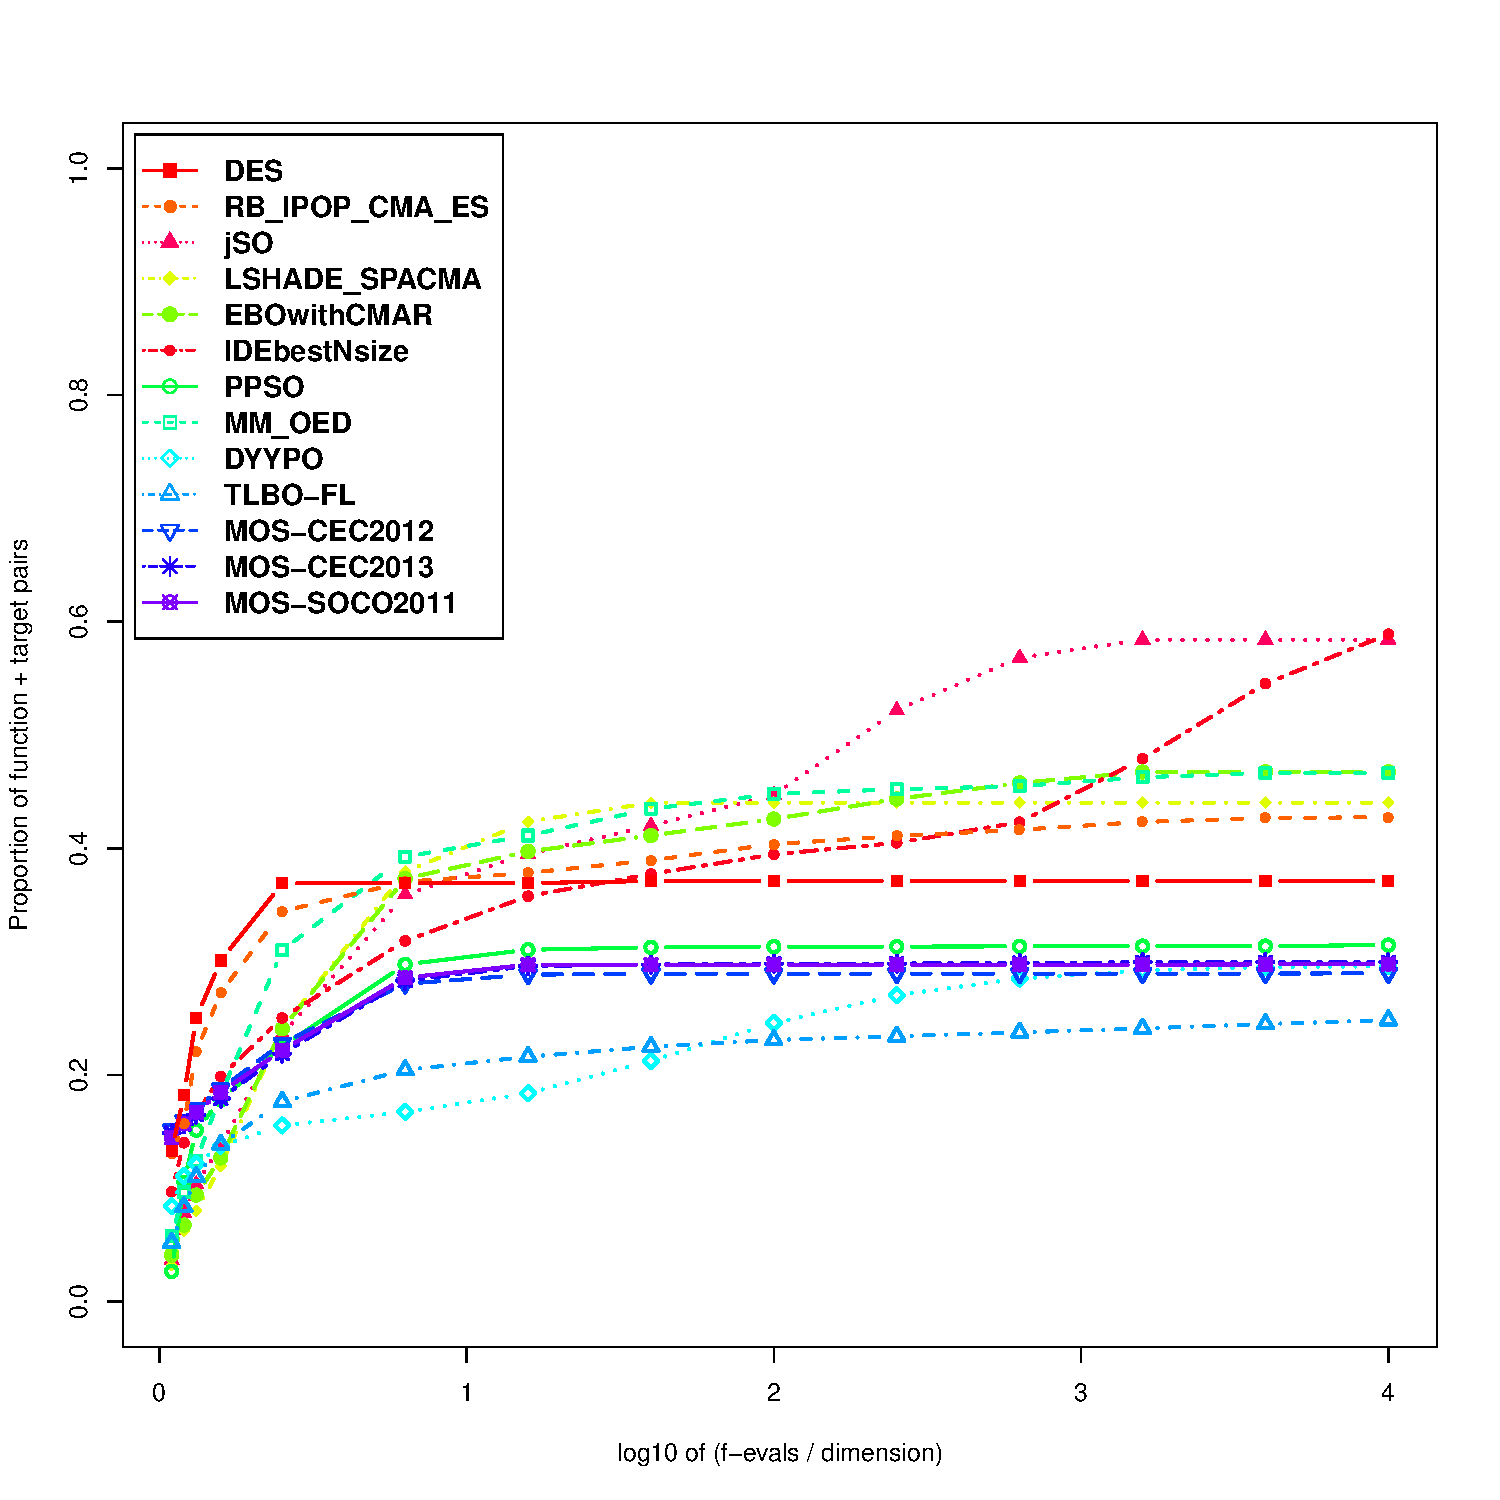
\includegraphics[height=0.9\linewidth,angle=90]{C:/Users/JS/Desktop/Doktorat/EvolutionAlgorithms/IEEEecdf/Plots/singlePlots/Problem=12,N=10.pdf} 
    		\caption{D=10} 
      	\end{minipage}%
	}
    \vspace{-12mm}
  \end{subfigure}%% 
  \begin{subfigure}[b]{0.5\linewidth}
    \centering
    \rotatebox[origin=c]{-90}{
        \begin{minipage}{1\linewidth}
            	\caption{D=30}
    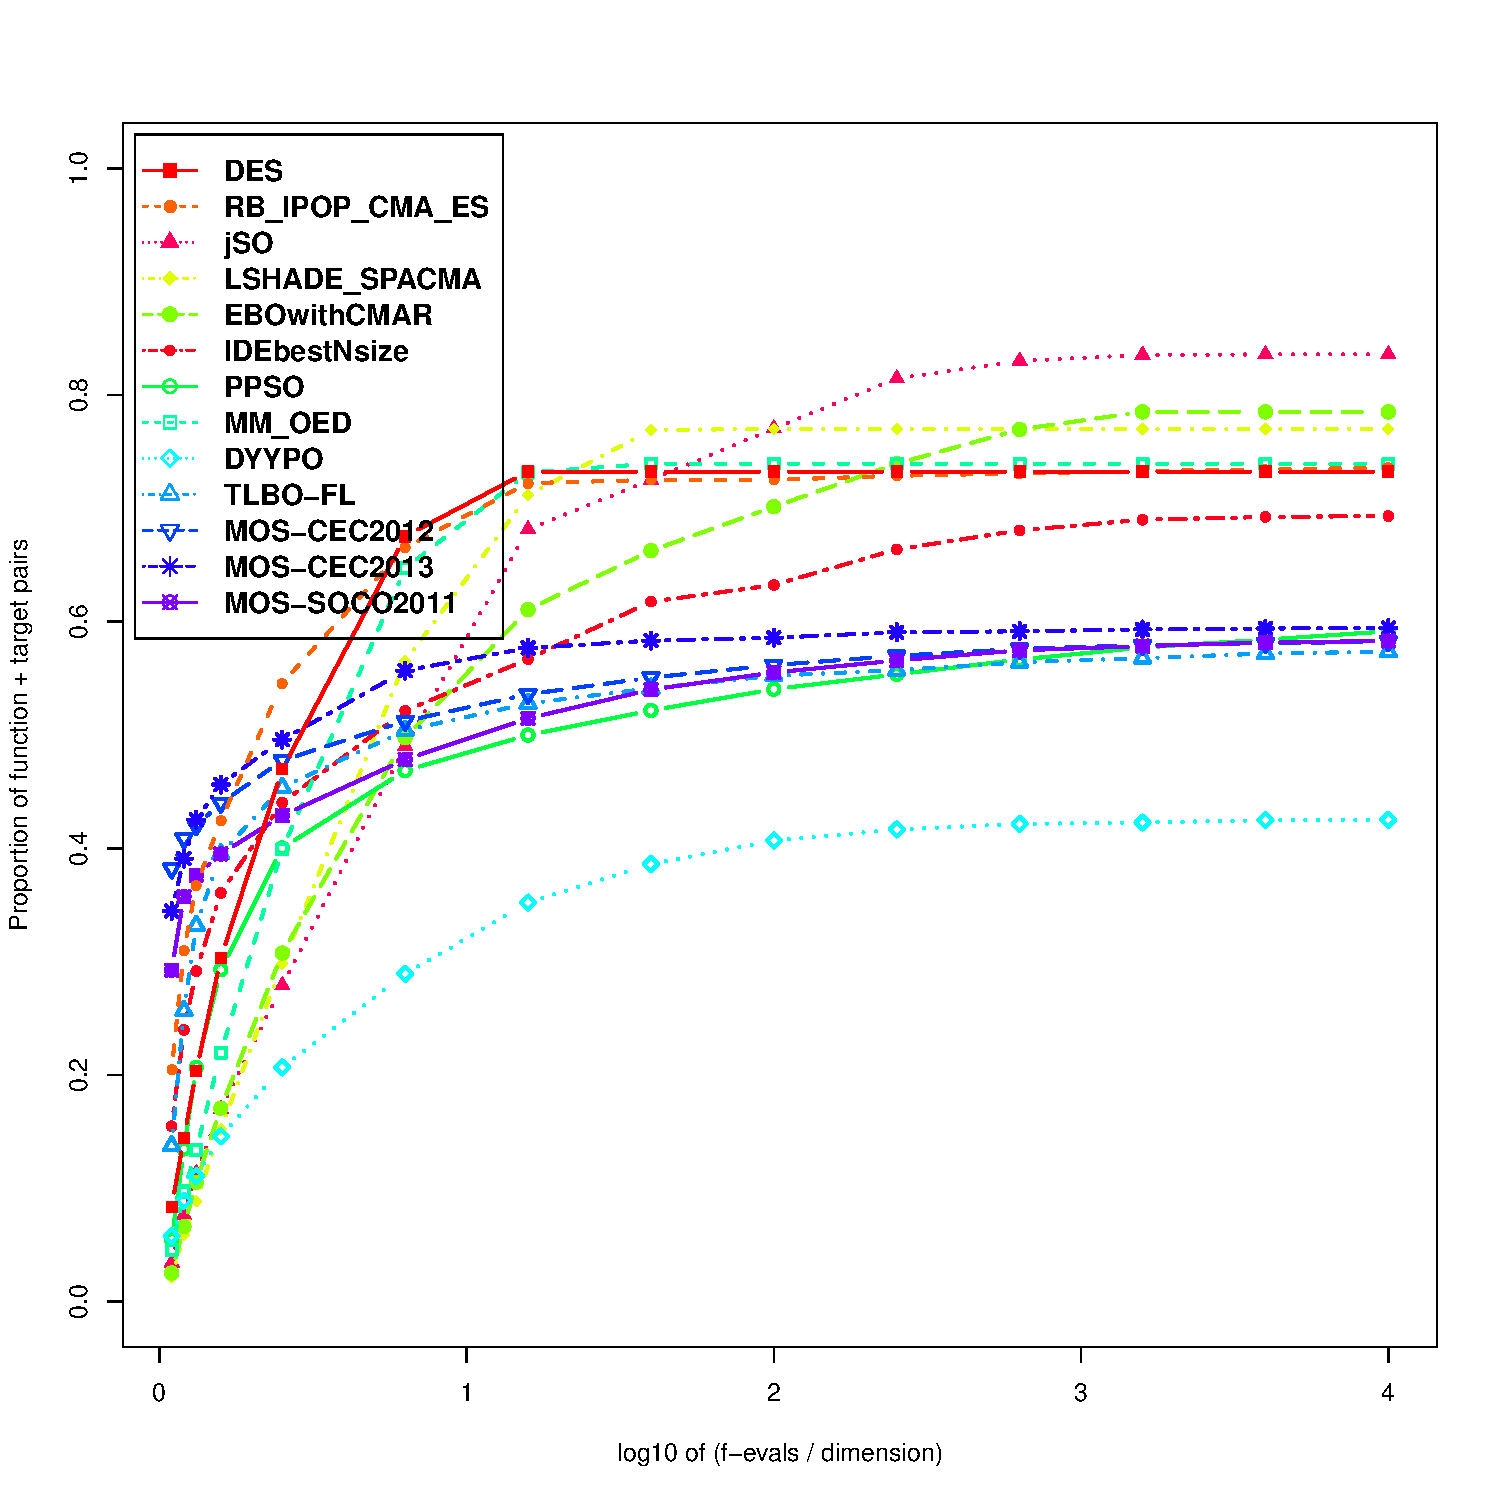
\includegraphics[height=0.9\linewidth,angle=90]{C:/Users/JS/Desktop/Doktorat/EvolutionAlgorithms/IEEEecdf/Plots/singlePlots/Problem=12,N=30.pdf} 
    	\end{minipage}%
	} 
    \vspace{-12mm}
  \end{subfigure} 
  \begin{subfigure}[b]{0.5\linewidth}
    \centering
    \rotatebox[origin=c]{-90}{
        \begin{minipage}{1\linewidth}
    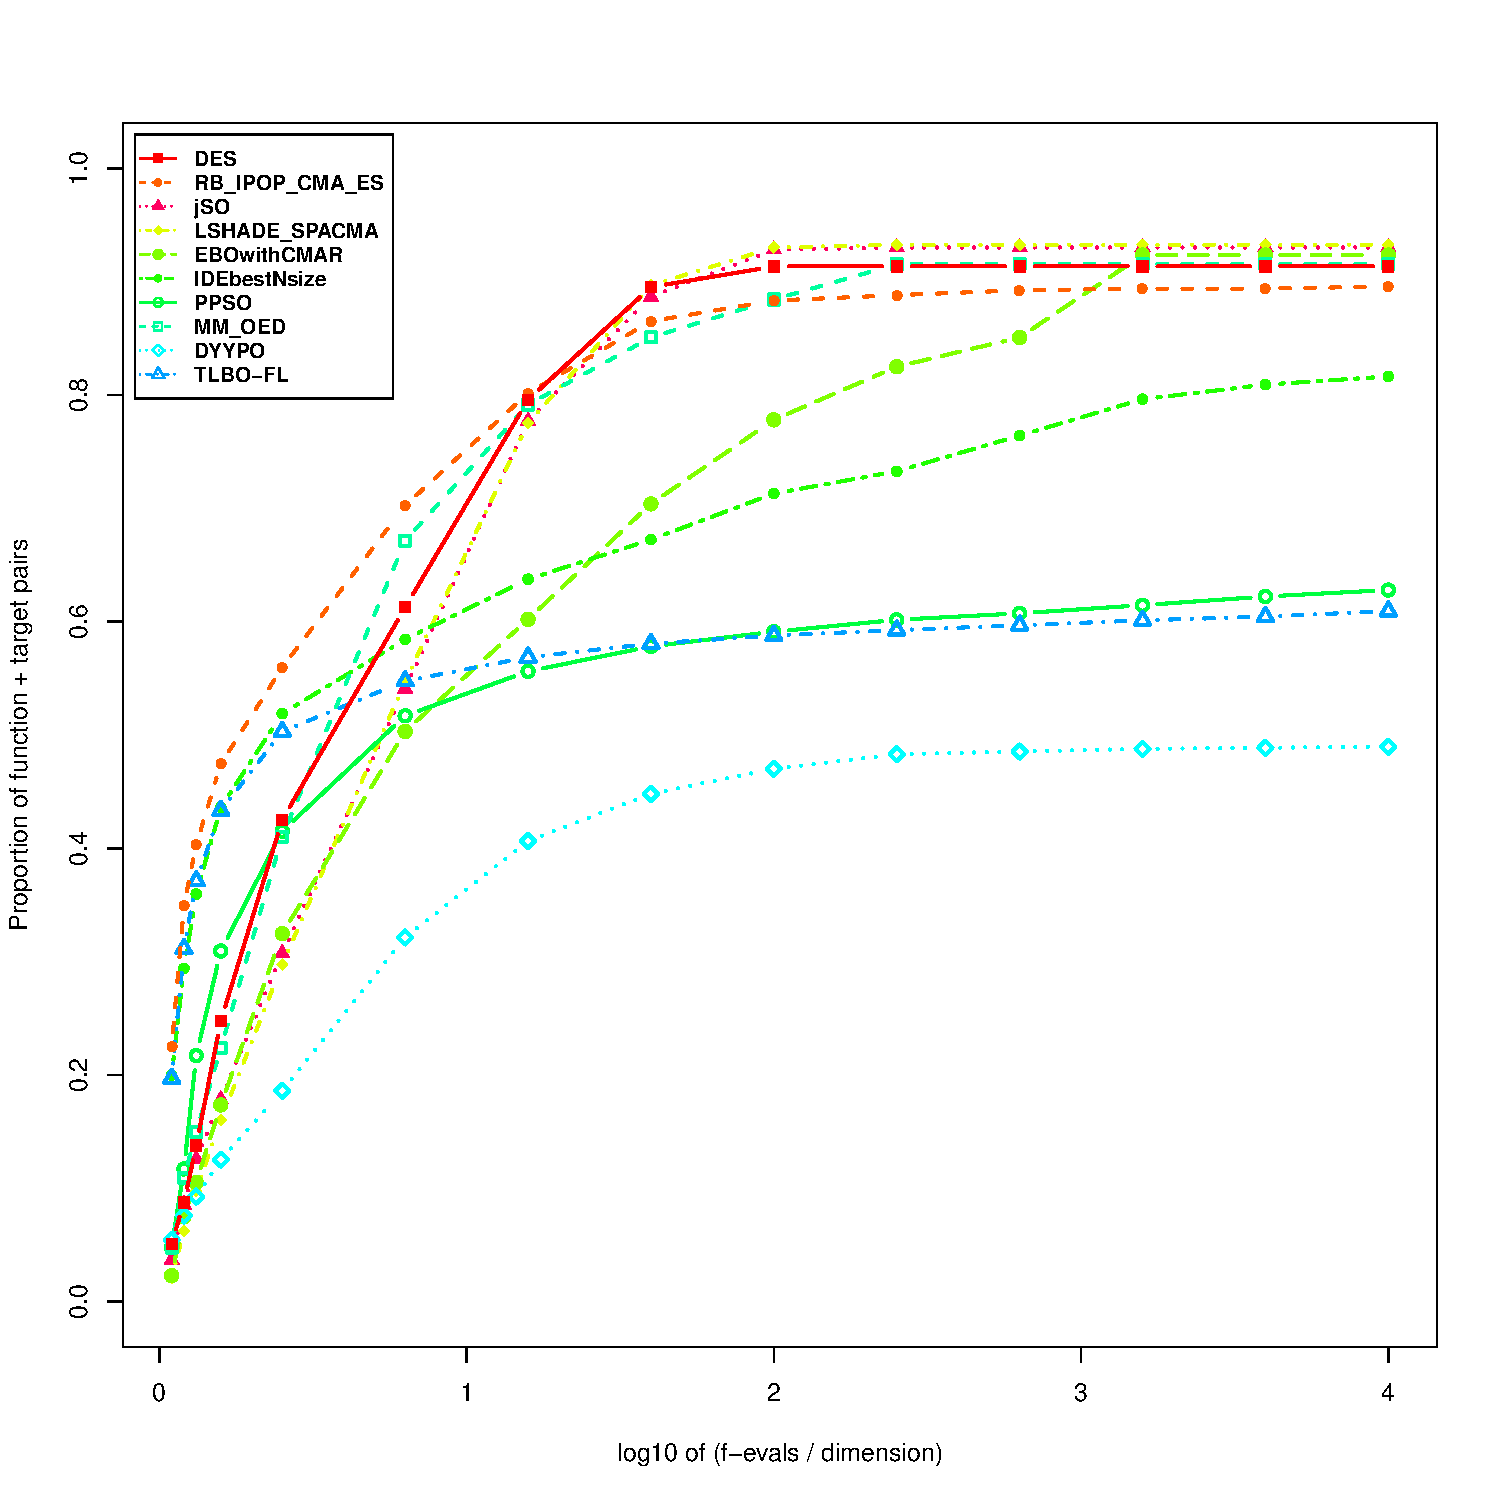
\includegraphics[height=0.9\linewidth,angle=90]{C:/Users/JS/Desktop/Doktorat/EvolutionAlgorithms/IEEEecdf/Plots/singlePlots/Problem=12,N=50.pdf} 
    	\caption{D=50}
    	\end{minipage}%
	}  
  \end{subfigure}%%
  \begin{subfigure}[b]{0.5\linewidth}
    \centering
    \rotatebox[origin=c]{-90}{
        \begin{minipage}{1\linewidth}
        \caption{D=100} 
    \includegraphics[height=0.9\linewidth,angle=90]{C:/Users/JS/Desktop/Doktorat/EvolutionAlgorithms/IEEEecdf/Plots/singlePlots/Problem=12,N=100.pdf}
    \end{minipage}%
	}   
  \end{subfigure} 
\end{figure}

\end{frame}


\begin{frame}
%\frametitle{CEC2017 Function 13}
\AddToShipoutPictureFG*{
    \AtPageUpperLeft{\put(-135,-12){
    \makebox[\paperwidth][r]{\textcolor{blue}{CEC2017 Function 13}}
    }
    }  
    }%

\begin{figure}[ht] 
    \vspace{-2mm}
\captionsetup[subfigure]{labelformat=empty}
  \begin{subfigure}[b]{0.5\linewidth}
    \centering
      \rotatebox[origin=c]{-90}{
        \begin{minipage}{1\linewidth}
    		\includegraphics[height=0.9\linewidth,angle=90]{C:/Users/JS/Desktop/Doktorat/EvolutionAlgorithms/IEEEecdf/Plots/singlePlots/Problem=13,N=10.pdf} 
    		\caption{D=10} 
      	\end{minipage}%
	}
    \vspace{-12mm}
  \end{subfigure}%% 
  \begin{subfigure}[b]{0.5\linewidth}
    \centering
    \rotatebox[origin=c]{-90}{
        \begin{minipage}{1\linewidth}
            	\caption{D=30}
    \includegraphics[height=0.9\linewidth,angle=90]{C:/Users/JS/Desktop/Doktorat/EvolutionAlgorithms/IEEEecdf/Plots/singlePlots/Problem=13,N=30.pdf} 
    	\end{minipage}%
	} 
    \vspace{-12mm}
  \end{subfigure} 
  \begin{subfigure}[b]{0.5\linewidth}
    \centering
    \rotatebox[origin=c]{-90}{
        \begin{minipage}{1\linewidth}
    \includegraphics[height=0.9\linewidth,angle=90]{C:/Users/JS/Desktop/Doktorat/EvolutionAlgorithms/IEEEecdf/Plots/singlePlots/Problem=13,N=50.pdf} 
    	\caption{D=50}
    	\end{minipage}%
	}  
  \end{subfigure}%%
  \begin{subfigure}[b]{0.5\linewidth}
    \centering
    \rotatebox[origin=c]{-90}{
        \begin{minipage}{1\linewidth}
        \caption{D=100} 
    \includegraphics[height=0.9\linewidth,angle=90]{C:/Users/JS/Desktop/Doktorat/EvolutionAlgorithms/IEEEecdf/Plots/singlePlots/Problem=13,N=100.pdf}
    \end{minipage}%
	}   
  \end{subfigure} 
\end{figure}

\end{frame}


\begin{frame}
%\frametitle{CEC2017 Function 14}
\AddToShipoutPictureFG*{
    \AtPageUpperLeft{\put(-135,-12){
    \makebox[\paperwidth][r]{\textcolor{blue}{CEC2017 Function 14}}
    }
    }  
    }%

\begin{figure}[ht] 
    \vspace{-2mm}
\captionsetup[subfigure]{labelformat=empty}
  \begin{subfigure}[b]{0.5\linewidth}
    \centering
      \rotatebox[origin=c]{-90}{
        \begin{minipage}{1\linewidth}
    		\includegraphics[height=0.9\linewidth,angle=90]{C:/Users/JS/Desktop/Doktorat/EvolutionAlgorithms/IEEEecdf/Plots/singlePlots/Problem=14,N=10.pdf} 
    		\caption{D=10} 
      	\end{minipage}%
	}
    \vspace{-12mm}
  \end{subfigure}%% 
  \begin{subfigure}[b]{0.5\linewidth}
    \centering
    \rotatebox[origin=c]{-90}{
        \begin{minipage}{1\linewidth}
            	\caption{D=30}
    \includegraphics[height=0.9\linewidth,angle=90]{C:/Users/JS/Desktop/Doktorat/EvolutionAlgorithms/IEEEecdf/Plots/singlePlots/Problem=14,N=30.pdf} 
    	\end{minipage}%
	} 
    \vspace{-12mm}
  \end{subfigure} 
  \begin{subfigure}[b]{0.5\linewidth}
    \centering
    \rotatebox[origin=c]{-90}{
        \begin{minipage}{1\linewidth}
    \includegraphics[height=0.9\linewidth,angle=90]{C:/Users/JS/Desktop/Doktorat/EvolutionAlgorithms/IEEEecdf/Plots/singlePlots/Problem=14,N=50.pdf} 
    	\caption{D=50}
    	\end{minipage}%
	}  
  \end{subfigure}%%
  \begin{subfigure}[b]{0.5\linewidth}
    \centering
    \rotatebox[origin=c]{-90}{
        \begin{minipage}{1\linewidth}
        \caption{D=100} 
    \includegraphics[height=0.9\linewidth,angle=90]{C:/Users/JS/Desktop/Doktorat/EvolutionAlgorithms/IEEEecdf/Plots/singlePlots/Problem=14,N=100.pdf}
    \end{minipage}%
	}   
  \end{subfigure} 
\end{figure}

\end{frame}


\begin{frame}
%\frametitle{CEC2017 Function 15}
\AddToShipoutPictureFG*{
    \AtPageUpperLeft{\put(-135,-12){
    \makebox[\paperwidth][r]{\textcolor{blue}{CEC2017 Function 15}}
    }
    }  
    }%

\begin{figure}[ht] 
    \vspace{-2mm}
\captionsetup[subfigure]{labelformat=empty}
  \begin{subfigure}[b]{0.5\linewidth}
    \centering
      \rotatebox[origin=c]{-90}{
        \begin{minipage}{1\linewidth}
    		\includegraphics[height=0.9\linewidth,angle=90]{C:/Users/JS/Desktop/Doktorat/EvolutionAlgorithms/IEEEecdf/Plots/singlePlots/Problem=15,N=10.pdf} 
    		\caption{D=10} 
      	\end{minipage}%
	}
    \vspace{-12mm}
  \end{subfigure}%% 
  \begin{subfigure}[b]{0.5\linewidth}
    \centering
    \rotatebox[origin=c]{-90}{
        \begin{minipage}{1\linewidth}
            	\caption{D=30}
    \includegraphics[height=0.9\linewidth,angle=90]{C:/Users/JS/Desktop/Doktorat/EvolutionAlgorithms/IEEEecdf/Plots/singlePlots/Problem=15,N=30.pdf} 
    	\end{minipage}%
	} 
    \vspace{-12mm}
  \end{subfigure} 
  \begin{subfigure}[b]{0.5\linewidth}
    \centering
    \rotatebox[origin=c]{-90}{
        \begin{minipage}{1\linewidth}
    \includegraphics[height=0.9\linewidth,angle=90]{C:/Users/JS/Desktop/Doktorat/EvolutionAlgorithms/IEEEecdf/Plots/singlePlots/Problem=15,N=50.pdf} 
    	\caption{D=50}
    	\end{minipage}%
	}  
  \end{subfigure}%%
  \begin{subfigure}[b]{0.5\linewidth}
    \centering
    \rotatebox[origin=c]{-90}{
        \begin{minipage}{1\linewidth}
        \caption{D=100} 
    \includegraphics[height=0.9\linewidth,angle=90]{C:/Users/JS/Desktop/Doktorat/EvolutionAlgorithms/IEEEecdf/Plots/singlePlots/Problem=15,N=100.pdf}
    \end{minipage}%
	}   
  \end{subfigure} 
\end{figure}

\end{frame}


\begin{frame}
%\frametitle{CEC2017 Function 16}
\AddToShipoutPictureFG*{
    \AtPageUpperLeft{\put(-135,-12){
    \makebox[\paperwidth][r]{\textcolor{blue}{CEC2017 Function 16}}
    }
    }  
    }%

\begin{figure}[ht] 
    \vspace{-2mm}
\captionsetup[subfigure]{labelformat=empty}
  \begin{subfigure}[b]{0.5\linewidth}
    \centering
      \rotatebox[origin=c]{-90}{
        \begin{minipage}{1\linewidth}
    		\includegraphics[height=0.9\linewidth,angle=90]{C:/Users/JS/Desktop/Doktorat/EvolutionAlgorithms/IEEEecdf/Plots/singlePlots/Problem=16,N=10.pdf} 
    		\caption{D=10} 
      	\end{minipage}%
	}
    \vspace{-12mm}
  \end{subfigure}%% 
  \begin{subfigure}[b]{0.5\linewidth}
    \centering
    \rotatebox[origin=c]{-90}{
        \begin{minipage}{1\linewidth}
            	\caption{D=30}
    \includegraphics[height=0.9\linewidth,angle=90]{C:/Users/JS/Desktop/Doktorat/EvolutionAlgorithms/IEEEecdf/Plots/singlePlots/Problem=16,N=30.pdf} 
    	\end{minipage}%
	} 
    \vspace{-12mm}
  \end{subfigure} 
  \begin{subfigure}[b]{0.5\linewidth}
    \centering
    \rotatebox[origin=c]{-90}{
        \begin{minipage}{1\linewidth}
    \includegraphics[height=0.9\linewidth,angle=90]{C:/Users/JS/Desktop/Doktorat/EvolutionAlgorithms/IEEEecdf/Plots/singlePlots/Problem=16,N=50.pdf} 
    	\caption{D=50}
    	\end{minipage}%
	}  
  \end{subfigure}%%
  \begin{subfigure}[b]{0.5\linewidth}
    \centering
    \rotatebox[origin=c]{-90}{
        \begin{minipage}{1\linewidth}
        \caption{D=100} 
    \includegraphics[height=0.9\linewidth,angle=90]{C:/Users/JS/Desktop/Doktorat/EvolutionAlgorithms/IEEEecdf/Plots/singlePlots/Problem=16,N=100.pdf}
    \end{minipage}%
	}   
  \end{subfigure} 
\end{figure}

\end{frame}


\begin{frame}
%\frametitle{CEC2017 Function 17}
\AddToShipoutPictureFG*{
    \AtPageUpperLeft{\put(-135,-12){
    \makebox[\paperwidth][r]{\textcolor{blue}{CEC2017 Function 17}}
    }
    }  
    }%

\begin{figure}[ht] 
    \vspace{-2mm}
\captionsetup[subfigure]{labelformat=empty}
  \begin{subfigure}[b]{0.5\linewidth}
    \centering
      \rotatebox[origin=c]{-90}{
        \begin{minipage}{1\linewidth}
    		\includegraphics[height=0.9\linewidth,angle=90]{C:/Users/JS/Desktop/Doktorat/EvolutionAlgorithms/IEEEecdf/Plots/singlePlots/Problem=17,N=10.pdf} 
    		\caption{D=10} 
      	\end{minipage}%
	}
    \vspace{-12mm}
  \end{subfigure}%% 
  \begin{subfigure}[b]{0.5\linewidth}
    \centering
    \rotatebox[origin=c]{-90}{
        \begin{minipage}{1\linewidth}
            	\caption{D=30}
    \includegraphics[height=0.9\linewidth,angle=90]{C:/Users/JS/Desktop/Doktorat/EvolutionAlgorithms/IEEEecdf/Plots/singlePlots/Problem=17,N=30.pdf} 
    	\end{minipage}%
	} 
    \vspace{-12mm}
  \end{subfigure} 
  \begin{subfigure}[b]{0.5\linewidth}
    \centering
    \rotatebox[origin=c]{-90}{
        \begin{minipage}{1\linewidth}
    \includegraphics[height=0.9\linewidth,angle=90]{C:/Users/JS/Desktop/Doktorat/EvolutionAlgorithms/IEEEecdf/Plots/singlePlots/Problem=17,N=50.pdf} 
    	\caption{D=50}
    	\end{minipage}%
	}  
  \end{subfigure}%%
  \begin{subfigure}[b]{0.5\linewidth}
    \centering
    \rotatebox[origin=c]{-90}{
        \begin{minipage}{1\linewidth}
        \caption{D=100} 
    \includegraphics[height=0.9\linewidth,angle=90]{C:/Users/JS/Desktop/Doktorat/EvolutionAlgorithms/IEEEecdf/Plots/singlePlots/Problem=17,N=100.pdf}
    \end{minipage}%
	}   
  \end{subfigure} 
\end{figure}

\end{frame}


\begin{frame}
%\frametitle{CEC2017 Function 18}
\AddToShipoutPictureFG*{
    \AtPageUpperLeft{\put(-135,-12){
    \makebox[\paperwidth][r]{\textcolor{blue}{CEC2017 Function 18}}
    }
    }  
    }%

\begin{figure}[ht] 
    \vspace{-2mm}
\captionsetup[subfigure]{labelformat=empty}
  \begin{subfigure}[b]{0.5\linewidth}
    \centering
      \rotatebox[origin=c]{-90}{
        \begin{minipage}{1\linewidth}
    		\includegraphics[height=0.9\linewidth,angle=90]{C:/Users/JS/Desktop/Doktorat/EvolutionAlgorithms/IEEEecdf/Plots/singlePlots/Problem=18,N=10.pdf} 
    		\caption{D=10} 
      	\end{minipage}%
	}
    \vspace{-12mm}
  \end{subfigure}%% 
  \begin{subfigure}[b]{0.5\linewidth}
    \centering
    \rotatebox[origin=c]{-90}{
        \begin{minipage}{1\linewidth}
            	\caption{D=30}
    \includegraphics[height=0.9\linewidth,angle=90]{C:/Users/JS/Desktop/Doktorat/EvolutionAlgorithms/IEEEecdf/Plots/singlePlots/Problem=18,N=30.pdf} 
    	\end{minipage}%
	} 
    \vspace{-12mm}
  \end{subfigure} 
  \begin{subfigure}[b]{0.5\linewidth}
    \centering
    \rotatebox[origin=c]{-90}{
        \begin{minipage}{1\linewidth}
    \includegraphics[height=0.9\linewidth,angle=90]{C:/Users/JS/Desktop/Doktorat/EvolutionAlgorithms/IEEEecdf/Plots/singlePlots/Problem=18,N=50.pdf} 
    	\caption{D=50}
    	\end{minipage}%
	}  
  \end{subfigure}%%
  \begin{subfigure}[b]{0.5\linewidth}
    \centering
    \rotatebox[origin=c]{-90}{
        \begin{minipage}{1\linewidth}
        \caption{D=100} 
    \includegraphics[height=0.9\linewidth,angle=90]{C:/Users/JS/Desktop/Doktorat/EvolutionAlgorithms/IEEEecdf/Plots/singlePlots/Problem=18,N=100.pdf}
    \end{minipage}%
	}   
  \end{subfigure} 
\end{figure}

\end{frame}

\begin{frame}
%\frametitle{CEC2017 Function 19}
\AddToShipoutPictureFG*{
    \AtPageUpperLeft{\put(-135,-12){
    \makebox[\paperwidth][r]{\textcolor{blue}{CEC2017 Function 19}}
    }
    }  
    }%

\begin{figure}[ht] 
    \vspace{-2mm}
\captionsetup[subfigure]{labelformat=empty}
  \begin{subfigure}[b]{0.5\linewidth}
    \centering
      \rotatebox[origin=c]{-90}{
        \begin{minipage}{1\linewidth}
    		\includegraphics[height=0.9\linewidth,angle=90]{C:/Users/JS/Desktop/Doktorat/EvolutionAlgorithms/IEEEecdf/Plots/singlePlots/Problem=19,N=10.pdf} 
    		\caption{D=10} 
      	\end{minipage}%
	}
    \vspace{-12mm}
  \end{subfigure}%% 
  \begin{subfigure}[b]{0.5\linewidth}
    \centering
    \rotatebox[origin=c]{-90}{
        \begin{minipage}{1\linewidth}
            	\caption{D=30}
    \includegraphics[height=0.9\linewidth,angle=90]{C:/Users/JS/Desktop/Doktorat/EvolutionAlgorithms/IEEEecdf/Plots/singlePlots/Problem=19,N=30.pdf} 
    	\end{minipage}%
	} 
    \vspace{-12mm}
  \end{subfigure} 
  \begin{subfigure}[b]{0.5\linewidth}
    \centering
    \rotatebox[origin=c]{-90}{
        \begin{minipage}{1\linewidth}
    \includegraphics[height=0.9\linewidth,angle=90]{C:/Users/JS/Desktop/Doktorat/EvolutionAlgorithms/IEEEecdf/Plots/singlePlots/Problem=19,N=50.pdf} 
    	\caption{D=50}
    	\end{minipage}%
	}  
  \end{subfigure}%%
  \begin{subfigure}[b]{0.5\linewidth}
    \centering
    \rotatebox[origin=c]{-90}{
        \begin{minipage}{1\linewidth}
        \caption{D=100} 
    \includegraphics[height=0.9\linewidth,angle=90]{C:/Users/JS/Desktop/Doktorat/EvolutionAlgorithms/IEEEecdf/Plots/singlePlots/Problem=19,N=100.pdf}
    \end{minipage}%
	}   
  \end{subfigure} 
\end{figure}

\end{frame}


\begin{frame}
%\frametitle{CEC2017 Function 20}
\AddToShipoutPictureFG*{
    \AtPageUpperLeft{\put(-135,-12){
    \makebox[\paperwidth][r]{\textcolor{blue}{CEC2017 Function 20}}
    }
    }  
    }%

\begin{figure}[ht] 
    \vspace{-2mm}
\captionsetup[subfigure]{labelformat=empty}
  \begin{subfigure}[b]{0.5\linewidth}
    \centering
      \rotatebox[origin=c]{-90}{
        \begin{minipage}{1\linewidth}
    		\includegraphics[height=0.9\linewidth,angle=90]{C:/Users/JS/Desktop/Doktorat/EvolutionAlgorithms/IEEEecdf/Plots/singlePlots/Problem=20,N=10.pdf} 
    		\caption{D=10} 
      	\end{minipage}%
	}
    \vspace{-12mm}
  \end{subfigure}%% 
  \begin{subfigure}[b]{0.5\linewidth}
    \centering
    \rotatebox[origin=c]{-90}{
        \begin{minipage}{1\linewidth}
            	\caption{D=30}
    \includegraphics[height=0.9\linewidth,angle=90]{C:/Users/JS/Desktop/Doktorat/EvolutionAlgorithms/IEEEecdf/Plots/singlePlots/Problem=20,N=30.pdf} 
    	\end{minipage}%
	} 
    \vspace{-12mm}
  \end{subfigure} 
  \begin{subfigure}[b]{0.5\linewidth}
    \centering
    \rotatebox[origin=c]{-90}{
        \begin{minipage}{1\linewidth}
    \includegraphics[height=0.9\linewidth,angle=90]{C:/Users/JS/Desktop/Doktorat/EvolutionAlgorithms/IEEEecdf/Plots/singlePlots/Problem=20,N=50.pdf} 
    	\caption{D=50}
    	\end{minipage}%
	}  
  \end{subfigure}%%
  \begin{subfigure}[b]{0.5\linewidth}
    \centering
    \rotatebox[origin=c]{-90}{
        \begin{minipage}{1\linewidth}
        \caption{D=100} 
    \includegraphics[height=0.9\linewidth,angle=90]{C:/Users/JS/Desktop/Doktorat/EvolutionAlgorithms/IEEEecdf/Plots/singlePlots/Problem=20,N=100.pdf}
    \end{minipage}%
	}   
  \end{subfigure} 
\end{figure}

\end{frame}


\begin{frame}
%\frametitle{CEC2017 Function 21}
\AddToShipoutPictureFG*{
    \AtPageUpperLeft{\put(-135,-12){
    \makebox[\paperwidth][r]{\textcolor{blue}{CEC2017 Function 21}}
    }
    }  
    }%

\begin{figure}[ht] 
    \vspace{-2mm}
\captionsetup[subfigure]{labelformat=empty}
  \begin{subfigure}[b]{0.5\linewidth}
    \centering
      \rotatebox[origin=c]{-90}{
        \begin{minipage}{1\linewidth}
    		\includegraphics[height=0.9\linewidth,angle=90]{C:/Users/JS/Desktop/Doktorat/EvolutionAlgorithms/IEEEecdf/Plots/singlePlots/Problem=21,N=10.pdf} 
    		\caption{D=10} 
      	\end{minipage}%
	}
    \vspace{-12mm}
  \end{subfigure}%% 
  \begin{subfigure}[b]{0.5\linewidth}
    \centering
    \rotatebox[origin=c]{-90}{
        \begin{minipage}{1\linewidth}
            	\caption{D=30}
    \includegraphics[height=0.9\linewidth,angle=90]{C:/Users/JS/Desktop/Doktorat/EvolutionAlgorithms/IEEEecdf/Plots/singlePlots/Problem=21,N=30.pdf} 
    	\end{minipage}%
	} 
    \vspace{-12mm}
  \end{subfigure} 
  \begin{subfigure}[b]{0.5\linewidth}
    \centering
    \rotatebox[origin=c]{-90}{
        \begin{minipage}{1\linewidth}
    \includegraphics[height=0.9\linewidth,angle=90]{C:/Users/JS/Desktop/Doktorat/EvolutionAlgorithms/IEEEecdf/Plots/singlePlots/Problem=21,N=50.pdf} 
    	\caption{D=50}
    	\end{minipage}%
	}  
  \end{subfigure}%%
  \begin{subfigure}[b]{0.5\linewidth}
    \centering
    \rotatebox[origin=c]{-90}{
        \begin{minipage}{1\linewidth}
        \caption{D=100} 
    \includegraphics[height=0.9\linewidth,angle=90]{C:/Users/JS/Desktop/Doktorat/EvolutionAlgorithms/IEEEecdf/Plots/singlePlots/Problem=21,N=100.pdf}
    \end{minipage}%
	}   
  \end{subfigure} 
\end{figure}

\end{frame}


\begin{frame}
%\frametitle{CEC2017 Function 22}
\AddToShipoutPictureFG*{
    \AtPageUpperLeft{\put(-135,-12){
    \makebox[\paperwidth][r]{\textcolor{blue}{CEC2017 Function 22}}
    }
    }  
    }%

\begin{figure}[ht] 
    \vspace{-2mm}
\captionsetup[subfigure]{labelformat=empty}
  \begin{subfigure}[b]{0.5\linewidth}
    \centering
      \rotatebox[origin=c]{-90}{
        \begin{minipage}{1\linewidth}
    		\includegraphics[height=0.9\linewidth,angle=90]{C:/Users/JS/Desktop/Doktorat/EvolutionAlgorithms/IEEEecdf/Plots/singlePlots/Problem=22,N=10.pdf} 
    		\caption{D=10} 
      	\end{minipage}%
	}
    \vspace{-12mm}
  \end{subfigure}%% 
  \begin{subfigure}[b]{0.5\linewidth}
    \centering
    \rotatebox[origin=c]{-90}{
        \begin{minipage}{1\linewidth}
            	\caption{D=30}
    \includegraphics[height=0.9\linewidth,angle=90]{C:/Users/JS/Desktop/Doktorat/EvolutionAlgorithms/IEEEecdf/Plots/singlePlots/Problem=22,N=30.pdf} 
    	\end{minipage}%
	} 
    \vspace{-12mm}
  \end{subfigure} 
  \begin{subfigure}[b]{0.5\linewidth}
    \centering
    \rotatebox[origin=c]{-90}{
        \begin{minipage}{1\linewidth}
    \includegraphics[height=0.9\linewidth,angle=90]{C:/Users/JS/Desktop/Doktorat/EvolutionAlgorithms/IEEEecdf/Plots/singlePlots/Problem=22,N=50.pdf} 
    	\caption{D=50}
    	\end{minipage}%
	}  
  \end{subfigure}%%
  \begin{subfigure}[b]{0.5\linewidth}
    \centering
    \rotatebox[origin=c]{-90}{
        \begin{minipage}{1\linewidth}
        \caption{D=100} 
    \includegraphics[height=0.9\linewidth,angle=90]{C:/Users/JS/Desktop/Doktorat/EvolutionAlgorithms/IEEEecdf/Plots/singlePlots/Problem=22,N=100.pdf}
    \end{minipage}%
	}   
  \end{subfigure} 
\end{figure}

\end{frame}


\begin{frame}
%\frametitle{CEC2017 Function 23}
\AddToShipoutPictureFG*{
    \AtPageUpperLeft{\put(-135,-12){
    \makebox[\paperwidth][r]{\textcolor{blue}{CEC2017 Function 23}}
    }
    }  
    }%

\begin{figure}[ht] 
    \vspace{-2mm}
\captionsetup[subfigure]{labelformat=empty}
  \begin{subfigure}[b]{0.5\linewidth}
    \centering
      \rotatebox[origin=c]{-90}{
        \begin{minipage}{1\linewidth}
    		\includegraphics[height=0.9\linewidth,angle=90]{C:/Users/JS/Desktop/Doktorat/EvolutionAlgorithms/IEEEecdf/Plots/singlePlots/Problem=23,N=10.pdf} 
    		\caption{D=10} 
      	\end{minipage}%
	}
    \vspace{-12mm}
  \end{subfigure}%% 
  \begin{subfigure}[b]{0.5\linewidth}
    \centering
    \rotatebox[origin=c]{-90}{
        \begin{minipage}{1\linewidth}
            	\caption{D=30}
    \includegraphics[height=0.9\linewidth,angle=90]{C:/Users/JS/Desktop/Doktorat/EvolutionAlgorithms/IEEEecdf/Plots/singlePlots/Problem=23,N=30.pdf} 
    	\end{minipage}%
	} 
    \vspace{-12mm}
  \end{subfigure} 
  \begin{subfigure}[b]{0.5\linewidth}
    \centering
    \rotatebox[origin=c]{-90}{
        \begin{minipage}{1\linewidth}
    \includegraphics[height=0.9\linewidth,angle=90]{C:/Users/JS/Desktop/Doktorat/EvolutionAlgorithms/IEEEecdf/Plots/singlePlots/Problem=23,N=50.pdf} 
    	\caption{D=50}
    	\end{minipage}%
	}  
  \end{subfigure}%%
  \begin{subfigure}[b]{0.5\linewidth}
    \centering
    \rotatebox[origin=c]{-90}{
        \begin{minipage}{1\linewidth}
        \caption{D=100} 
    \includegraphics[height=0.9\linewidth,angle=90]{C:/Users/JS/Desktop/Doktorat/EvolutionAlgorithms/IEEEecdf/Plots/singlePlots/Problem=23,N=100.pdf}
    \end{minipage}%
	}   
  \end{subfigure} 
\end{figure}

\end{frame}



\begin{frame}
%\frametitle{CEC2017 Function 24}
\AddToShipoutPictureFG*{
    \AtPageUpperLeft{\put(-135,-12){
    \makebox[\paperwidth][r]{\textcolor{blue}{CEC2017 Function 24}}
    }
    }  
    }%

\begin{figure}[ht] 
    \vspace{-2mm}
\captionsetup[subfigure]{labelformat=empty}
  \begin{subfigure}[b]{0.5\linewidth}
    \centering
      \rotatebox[origin=c]{-90}{
        \begin{minipage}{1\linewidth}
    		\includegraphics[height=0.9\linewidth,angle=90]{C:/Users/JS/Desktop/Doktorat/EvolutionAlgorithms/IEEEecdf/Plots/singlePlots/Problem=24,N=10.pdf} 
    		\caption{D=10} 
      	\end{minipage}%
	}
    \vspace{-12mm}
  \end{subfigure}%% 
  \begin{subfigure}[b]{0.5\linewidth}
    \centering
    \rotatebox[origin=c]{-90}{
        \begin{minipage}{1\linewidth}
            	\caption{D=30}
    \includegraphics[height=0.9\linewidth,angle=90]{C:/Users/JS/Desktop/Doktorat/EvolutionAlgorithms/IEEEecdf/Plots/singlePlots/Problem=24,N=30.pdf} 
    	\end{minipage}%
	} 
    \vspace{-12mm}
  \end{subfigure} 
  \begin{subfigure}[b]{0.5\linewidth}
    \centering
    \rotatebox[origin=c]{-90}{
        \begin{minipage}{1\linewidth}
    \includegraphics[height=0.9\linewidth,angle=90]{C:/Users/JS/Desktop/Doktorat/EvolutionAlgorithms/IEEEecdf/Plots/singlePlots/Problem=24,N=50.pdf} 
    	\caption{D=50}
    	\end{minipage}%
	}  
  \end{subfigure}%%
  \begin{subfigure}[b]{0.5\linewidth}
    \centering
    \rotatebox[origin=c]{-90}{
        \begin{minipage}{1\linewidth}
        \caption{D=100} 
    \includegraphics[height=0.9\linewidth,angle=90]{C:/Users/JS/Desktop/Doktorat/EvolutionAlgorithms/IEEEecdf/Plots/singlePlots/Problem=24,N=100.pdf}
    \end{minipage}%
	}   
  \end{subfigure} 
\end{figure}

\end{frame}


\begin{frame}
%\frametitle{CEC2017 Function 25}
\AddToShipoutPictureFG*{
    \AtPageUpperLeft{\put(-135,-12){
    \makebox[\paperwidth][r]{\textcolor{blue}{CEC2017 Function 25}}
    }
    }  
    }%

\begin{figure}[ht] 
    \vspace{-2mm}
\captionsetup[subfigure]{labelformat=empty}
  \begin{subfigure}[b]{0.5\linewidth}
    \centering
      \rotatebox[origin=c]{-90}{
        \begin{minipage}{1\linewidth}
    		\includegraphics[height=0.9\linewidth,angle=90]{C:/Users/JS/Desktop/Doktorat/EvolutionAlgorithms/IEEEecdf/Plots/singlePlots/Problem=25,N=10.pdf} 
    		\caption{D=10} 
      	\end{minipage}%
	}
    \vspace{-12mm}
  \end{subfigure}%% 
  \begin{subfigure}[b]{0.5\linewidth}
    \centering
    \rotatebox[origin=c]{-90}{
        \begin{minipage}{1\linewidth}
            	\caption{D=30}
    \includegraphics[height=0.9\linewidth,angle=90]{C:/Users/JS/Desktop/Doktorat/EvolutionAlgorithms/IEEEecdf/Plots/singlePlots/Problem=25,N=30.pdf} 
    	\end{minipage}%
	} 
    \vspace{-12mm}
  \end{subfigure} 
  \begin{subfigure}[b]{0.5\linewidth}
    \centering
    \rotatebox[origin=c]{-90}{
        \begin{minipage}{1\linewidth}
    \includegraphics[height=0.9\linewidth,angle=90]{C:/Users/JS/Desktop/Doktorat/EvolutionAlgorithms/IEEEecdf/Plots/singlePlots/Problem=25,N=50.pdf} 
    	\caption{D=50}
    	\end{minipage}%
	}  
  \end{subfigure}%%
  \begin{subfigure}[b]{0.5\linewidth}
    \centering
    \rotatebox[origin=c]{-90}{
        \begin{minipage}{1\linewidth}
        \caption{D=100} 
    \includegraphics[height=0.9\linewidth,angle=90]{C:/Users/JS/Desktop/Doktorat/EvolutionAlgorithms/IEEEecdf/Plots/singlePlots/Problem=25,N=100.pdf}
    \end{minipage}%
	}   
  \end{subfigure} 
\end{figure}

\end{frame}


\begin{frame}
%\frametitle{CEC2017 Function 26}
\AddToShipoutPictureFG*{
    \AtPageUpperLeft{\put(-135,-12){
    \makebox[\paperwidth][r]{\textcolor{blue}{CEC2017 Function 26}}
    }
    }  
    }%

\begin{figure}[ht] 
    \vspace{-2mm}
\captionsetup[subfigure]{labelformat=empty}
  \begin{subfigure}[b]{0.5\linewidth}
    \centering
      \rotatebox[origin=c]{-90}{
        \begin{minipage}{1\linewidth}
    		\includegraphics[height=0.9\linewidth,angle=90]{C:/Users/JS/Desktop/Doktorat/EvolutionAlgorithms/IEEEecdf/Plots/singlePlots/Problem=26,N=10.pdf} 
    		\caption{D=10} 
      	\end{minipage}%
	}
    \vspace{-12mm}
  \end{subfigure}%% 
  \begin{subfigure}[b]{0.5\linewidth}
    \centering
    \rotatebox[origin=c]{-90}{
        \begin{minipage}{1\linewidth}
            	\caption{D=30}
    \includegraphics[height=0.9\linewidth,angle=90]{C:/Users/JS/Desktop/Doktorat/EvolutionAlgorithms/IEEEecdf/Plots/singlePlots/Problem=26,N=30.pdf} 
    	\end{minipage}%
	} 
    \vspace{-12mm}
  \end{subfigure} 
  \begin{subfigure}[b]{0.5\linewidth}
    \centering
    \rotatebox[origin=c]{-90}{
        \begin{minipage}{1\linewidth}
    \includegraphics[height=0.9\linewidth,angle=90]{C:/Users/JS/Desktop/Doktorat/EvolutionAlgorithms/IEEEecdf/Plots/singlePlots/Problem=26,N=50.pdf} 
    	\caption{D=50}
    	\end{minipage}%
	}  
  \end{subfigure}%%
  \begin{subfigure}[b]{0.5\linewidth}
    \centering
    \rotatebox[origin=c]{-90}{
        \begin{minipage}{1\linewidth}
        \caption{D=100} 
    \includegraphics[height=0.9\linewidth,angle=90]{C:/Users/JS/Desktop/Doktorat/EvolutionAlgorithms/IEEEecdf/Plots/singlePlots/Problem=26,N=100.pdf}
    \end{minipage}%
	}   
  \end{subfigure} 
\end{figure}

\end{frame}


\begin{frame}
%\frametitle{CEC2017 Function 27}
\AddToShipoutPictureFG*{
    \AtPageUpperLeft{\put(-135,-12){
    \makebox[\paperwidth][r]{\textcolor{blue}{CEC2017 Function 27}}
    }
    }  
    }%

\begin{figure}[ht] 
    \vspace{-2mm}
\captionsetup[subfigure]{labelformat=empty}
  \begin{subfigure}[b]{0.5\linewidth}
    \centering
      \rotatebox[origin=c]{-90}{
        \begin{minipage}{1\linewidth}
    		\includegraphics[height=0.9\linewidth,angle=90]{C:/Users/JS/Desktop/Doktorat/EvolutionAlgorithms/IEEEecdf/Plots/singlePlots/Problem=27,N=10.pdf} 
    		\caption{D=10} 
      	\end{minipage}%
	}
    \vspace{-12mm}
  \end{subfigure}%% 
  \begin{subfigure}[b]{0.5\linewidth}
    \centering
    \rotatebox[origin=c]{-90}{
        \begin{minipage}{1\linewidth}
            	\caption{D=30}
    \includegraphics[height=0.9\linewidth,angle=90]{C:/Users/JS/Desktop/Doktorat/EvolutionAlgorithms/IEEEecdf/Plots/singlePlots/Problem=27,N=30.pdf} 
    	\end{minipage}%
	} 
    \vspace{-12mm}
  \end{subfigure} 
  \begin{subfigure}[b]{0.5\linewidth}
    \centering
    \rotatebox[origin=c]{-90}{
        \begin{minipage}{1\linewidth}
    \includegraphics[height=0.9\linewidth,angle=90]{C:/Users/JS/Desktop/Doktorat/EvolutionAlgorithms/IEEEecdf/Plots/singlePlots/Problem=27,N=50.pdf} 
    	\caption{D=50}
    	\end{minipage}%
	}  
  \end{subfigure}%%
  \begin{subfigure}[b]{0.5\linewidth}
    \centering
    \rotatebox[origin=c]{-90}{
        \begin{minipage}{1\linewidth}
        \caption{D=100} 
    \includegraphics[height=0.9\linewidth,angle=90]{C:/Users/JS/Desktop/Doktorat/EvolutionAlgorithms/IEEEecdf/Plots/singlePlots/Problem=27,N=100.pdf}
    \end{minipage}%
	}   
  \end{subfigure} 
\end{figure}

\end{frame}


\begin{frame}
%\frametitle{CEC2017 Function 28}
\AddToShipoutPictureFG*{
    \AtPageUpperLeft{\put(-135,-12){
    \makebox[\paperwidth][r]{\textcolor{blue}{CEC2017 Function 28}}
    }
    }  
    }%

\begin{figure}[ht] 
    \vspace{-2mm}
\captionsetup[subfigure]{labelformat=empty}
  \begin{subfigure}[b]{0.5\linewidth}
    \centering
      \rotatebox[origin=c]{-90}{
        \begin{minipage}{1\linewidth}
    		\includegraphics[height=0.9\linewidth,angle=90]{C:/Users/JS/Desktop/Doktorat/EvolutionAlgorithms/IEEEecdf/Plots/singlePlots/Problem=28,N=10.pdf} 
    		\caption{D=10} 
      	\end{minipage}%
	}
    \vspace{-12mm}
  \end{subfigure}%% 
  \begin{subfigure}[b]{0.5\linewidth}
    \centering
    \rotatebox[origin=c]{-90}{
        \begin{minipage}{1\linewidth}
            	\caption{D=30}
    \includegraphics[height=0.9\linewidth,angle=90]{C:/Users/JS/Desktop/Doktorat/EvolutionAlgorithms/IEEEecdf/Plots/singlePlots/Problem=28,N=30.pdf} 
    	\end{minipage}%
	} 
    \vspace{-12mm}
  \end{subfigure} 
  \begin{subfigure}[b]{0.5\linewidth}
    \centering
    \rotatebox[origin=c]{-90}{
        \begin{minipage}{1\linewidth}
    \includegraphics[height=0.9\linewidth,angle=90]{C:/Users/JS/Desktop/Doktorat/EvolutionAlgorithms/IEEEecdf/Plots/singlePlots/Problem=28,N=50.pdf} 
    	\caption{D=50}
    	\end{minipage}%
	}  
  \end{subfigure}%%
  \begin{subfigure}[b]{0.5\linewidth}
    \centering
    \rotatebox[origin=c]{-90}{
        \begin{minipage}{1\linewidth}
        \caption{D=100} 
    \includegraphics[height=0.9\linewidth,angle=90]{C:/Users/JS/Desktop/Doktorat/EvolutionAlgorithms/IEEEecdf/Plots/singlePlots/Problem=28,N=100.pdf}
    \end{minipage}%
	}   
  \end{subfigure} 
\end{figure}

\end{frame}


\begin{frame}
%\frametitle{CEC2017 Function 29}
\AddToShipoutPictureFG*{
    \AtPageUpperLeft{\put(-135,-12){
    \makebox[\paperwidth][r]{\textcolor{blue}{CEC2017 Function 29}}
    }
    }  
    }%

\begin{figure}[ht] 
    \vspace{-2mm}
\captionsetup[subfigure]{labelformat=empty}
  \begin{subfigure}[b]{0.5\linewidth}
    \centering
      \rotatebox[origin=c]{-90}{
        \begin{minipage}{1\linewidth}
    		\includegraphics[height=0.9\linewidth,angle=90]{C:/Users/JS/Desktop/Doktorat/EvolutionAlgorithms/IEEEecdf/Plots/singlePlots/Problem=29,N=10.pdf} 
    		\caption{D=10} 
      	\end{minipage}%
	}
    \vspace{-12mm}
  \end{subfigure}%% 
  \begin{subfigure}[b]{0.5\linewidth}
    \centering
    \rotatebox[origin=c]{-90}{
        \begin{minipage}{1\linewidth}
            	\caption{D=30}
    \includegraphics[height=0.9\linewidth,angle=90]{C:/Users/JS/Desktop/Doktorat/EvolutionAlgorithms/IEEEecdf/Plots/singlePlots/Problem=29,N=30.pdf} 
    	\end{minipage}%
	} 
    \vspace{-12mm}
  \end{subfigure} 
  \begin{subfigure}[b]{0.5\linewidth}
    \centering
    \rotatebox[origin=c]{-90}{
        \begin{minipage}{1\linewidth}
    \includegraphics[height=0.9\linewidth,angle=90]{C:/Users/JS/Desktop/Doktorat/EvolutionAlgorithms/IEEEecdf/Plots/singlePlots/Problem=29,N=50.pdf} 
    	\caption{D=50}
    	\end{minipage}%
	}  
  \end{subfigure}%%
  \begin{subfigure}[b]{0.5\linewidth}
    \centering
    \rotatebox[origin=c]{-90}{
        \begin{minipage}{1\linewidth}
        \caption{D=100} 
    \includegraphics[height=0.9\linewidth,angle=90]{C:/Users/JS/Desktop/Doktorat/EvolutionAlgorithms/IEEEecdf/Plots/singlePlots/Problem=29,N=100.pdf}
    \end{minipage}%
	}   
  \end{subfigure} 
\end{figure}

\end{frame}

\begin{frame}
%\frametitle{CEC2017 Function 30}
\AddToShipoutPictureFG*{
    \AtPageUpperLeft{\put(-135,-12){
    \makebox[\paperwidth][r]{\textcolor{blue}{CEC2017 Function 30}}
    }
    }  
    }%

\begin{figure}[ht] 
    \vspace{-2mm}
\captionsetup[subfigure]{labelformat=empty}
  \begin{subfigure}[b]{0.5\linewidth}
    \centering
      \rotatebox[origin=c]{-90}{
        \begin{minipage}{1\linewidth}
    		\includegraphics[height=0.9\linewidth,angle=90]{C:/Users/JS/Desktop/Doktorat/EvolutionAlgorithms/IEEEecdf/Plots/singlePlots/Problem=30,N=10.pdf} 
    		\caption{D=10} 
      	\end{minipage}%
	}
    \vspace{-12mm}
  \end{subfigure}%% 
  \begin{subfigure}[b]{0.5\linewidth}
    \centering
    \rotatebox[origin=c]{-90}{
        \begin{minipage}{1\linewidth}
            	\caption{D=30}
    \includegraphics[height=0.9\linewidth,angle=90]{C:/Users/JS/Desktop/Doktorat/EvolutionAlgorithms/IEEEecdf/Plots/singlePlots/Problem=30,N=30.pdf} 
    	\end{minipage}%
	} 
    \vspace{-12mm}
  \end{subfigure} 
  \begin{subfigure}[b]{0.5\linewidth}
    \centering
    \rotatebox[origin=c]{-90}{
        \begin{minipage}{1\linewidth}
    \includegraphics[height=0.9\linewidth,angle=90]{C:/Users/JS/Desktop/Doktorat/EvolutionAlgorithms/IEEEecdf/Plots/singlePlots/Problem=30,N=50.pdf} 
    	\caption{D=50}
    	\end{minipage}%
	}  
  \end{subfigure}%%
  \begin{subfigure}[b]{0.5\linewidth}
    \centering
    \rotatebox[origin=c]{-90}{
        \begin{minipage}{1\linewidth}
        \caption{D=100} 
    \includegraphics[height=0.9\linewidth,angle=90]{C:/Users/JS/Desktop/Doktorat/EvolutionAlgorithms/IEEEecdf/Plots/singlePlots/Problem=30,N=100.pdf}
    \end{minipage}%
	}   
  \end{subfigure} 
\end{figure}

\end{frame}

\end{document}
